\chapter{M�todos}
\label{metodosec}

Este cap�tulo descreve todos os procedimentos de projeto e testes, dentre outros, empregados visando a obten��o do resultado final deste trabalho. Os procedimentos aqui empregados s�o embasados na teoria apresentada no cap�tulo \ref{EmbasamentoTeorico}. Cabe salientar que, embora este seja um projeto de integra��o entre \textit{mec�nica}, \textit{hardware} e \textit{software}, os esfor�os de desenvolvimento foram concentrados na �rea de desenvolvimento de \textit{softwares}, desde o servidor web e o algoritmo de controle implementados em Node.js, at� a aplica��o de usu�rio, escrita em diversas linguagens, de programa��o ou n�o --- a exemplo de HTML e CSS. A figura \ref{blocos} apresenta uma vis�o geral do sistema, que compreende parte mec�nica, \textit{hardware} e \textit{software}.

\begin{figure}[H]
	\centering
	\includegraphics[scale=0.40]{./Resources/diag_geral.png}
	\captionsetup{justification=centering}
	\caption[Diagrama em blocos do projeto]{Diagrama em blocos do projeto}
	\label{blocos}
\end{figure}

%%%%%%%%%%%%%%%%%%%%%%%%%%%%%%%%%%%%%%%%%%%%%%%%%%%%%%%%%%%%%%%%%%%

\section{Estrutura mec�nica}
\label{estmec}
Para o projeto da parte mec�nica, em primeiro lugar foi concebida uma configura��o de sistema baseada tanto na literatura dispon�vel quanto em projetos de sistemas comerciais de produ��o de cerveja: um sistema de duas panelas an�logas � MT e ao BK, sendo que durante o processo de cozimento do mosto, o BK pudesse ser utilizado como HLT. Para atender a esta especifica��o, fez-se necess�rio o projeto de um sistema de recircula��o entre as duas panelas. Observa-se que esta proposta representa um h�brido entre o sistema de 3 panelas tradicional - que consiste de uma panela para mostura��o, uma para lavagem dos gr�os, ou \textit{sparging}, e uma para fervura; e o sistema popularizado pela Braumeister, composto de 1 panela, com recircula��o. Esta abordagem permitiu a economia financeira e simplifica��o mec�nica do sistema de tr�s panelas com o benef�cio do \textit{sparging} inexistente no sistema de uma panela.

\subsection{Funcionamento da estrutura}

Na figura \ref{esboco} � apresentada uma representa��o esquem�tica da parte funcional.

\begin{figure}[H]
	\centering
	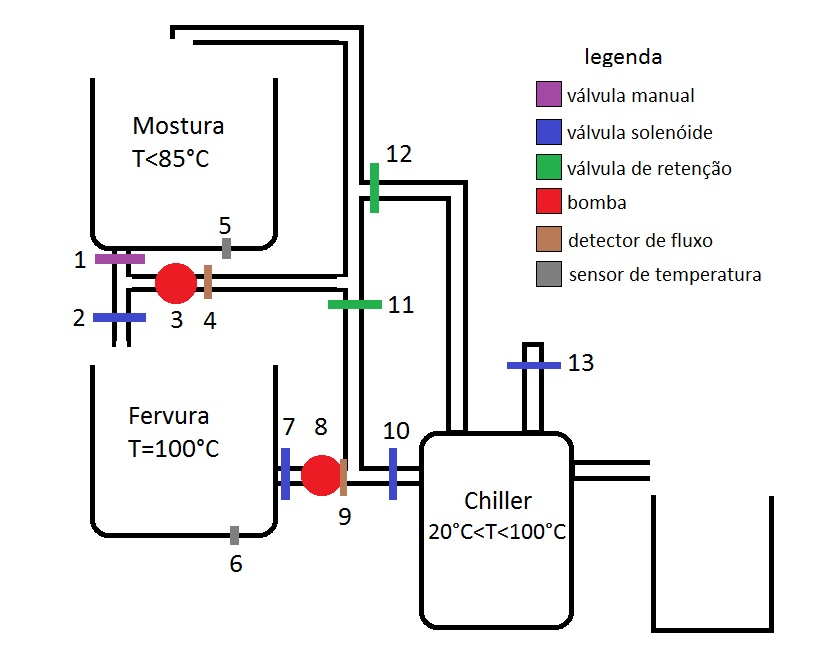
\includegraphics[scale=0.55]{./Resources/esb_mec.jpg}
	\captionsetup{justification=centering}
	\caption[Representa��o esquem�tica da estrutura mec�nica]{Representa��o esquem�tica da estrutura mec�nica}
	\label{esboco}
\end{figure}

Na panela superior ou MT, rotulada como \textit{Mostura}, os gr�os s�o adicionados ap�s o aquecimento inicial da �gua:

\begin{itemize}
	\item A v�lvula 1 � uma v�lvula manual do tipo esfera, com passagem plena. Durante a opera��o do equipamento ela deve ficar sempre aberta, portanto seu uso � realizado somente em caso de emerg�ncias.
	\item Ap�s a adi��o dos gr�os, a bomba 3 � ligada para que o l�quido da panela seja recirculado. As v�lvulas de reten��o 11 e 12 n�o permitem que o l�quido passe por elas, portanto h� somente um caminho poss�vel para este, que � ascender pela tubula��o at� entrar novamente na MT. Note-se que n�o h� v�lvula automatizada na sa�da da MT, uma vez que o mosto fica em recircula��o constante ao longo do processo de cozimento.
	\item Ap�s a mostura a bomba 3 � desligada e a v�lvula solen�ide 2 � aberta, escoando o l�quido para a panela de fervura BK. Simult�neamente, a v�lvula solen�ide 7 e a bomba 8 s�o ativadas, fazendo com que a �gua de lavagem presente na BK/HLT flua pela tubula��o at� a MT, iniciando o processo de \textit{sparging}. Durante um tempo predefinido, o mosto e a �gua de lavagem recirculam pelas duas panelas e se misturam.
	\item Durante a fervura, as v�lvulas 2 e 7 s�o fechadas. Neste per�odo, os gr�os drenados que est�o na MT devem ser retirados manualmente, j� que ela ser� usada posteriormente para armazenamento da �gua de esfriamento do mosto --- �gua usada para limpeza do sistema e que reduz a produ��o de efluentes do mesmo.
	\item Ap�s a fervura, as v�lvulas solen�ides 7 e 10 s�o ativadas, permitindo o escoamento do l�quido para o trocador de calor. Simult�neamente a v�lvula solen�ide 13 � aberta e �gua fria circula em contra-fluxo para resfriar o mosto. Esta �gua sai quente do trocador de calor e passa pela v�lvula de reten��o 12, preenchendo a parte superior da tubula��o e sendo armazenada na MT para posterior limpeza do sistema.
	\item O mosto que sai resfriado do \textit{chiller} cai no balde de fermenta��o. Neste processo o l�quido entra em contato com o ar, o que � n�o somente desej�vel como essencial para o sucesso da fermenta��o, portanto esta � a �ltima parte automatizada que tem rela��o com a cerveja. Uma solu��o futura e que permite automa��o desta transi��o � o uso de um aerador em conjunto com um tanque de fermenta��o selado.
	\item Por fim, a �gua armazenada na MT � aquecida e recirculada pelo sistema, promovendo uma limpeza preliminar deste.
\end{itemize}

\pagebreak

Para o bom funcionamento do sistema proposto, algumas condi��es devem ser atendidas:

\begin{itemize}
	\item Se o volume total de l�quido nas duas panelas ao final da mostura exceder o volume da BK, ela transbordar�. Por este motivo � importante que exista um sistema de detec��o de transbordo. Ainda assim, deve-se requisitar que o usu�rio do sistema calcule corretamente as propor��es da receita, pois mesmo que seja aplicado um sistema autom�tico anti-transbordo, ocorrer� perda de insumos devido ao ac�mulo de mosto inutiliz�vel na MT em caso de erro.
	\item S�o necess�rios filtros de material particulado na sa�da das panelas para o bom funcionamento das v�lvulas e bombas \cite{danfoss_solenoid}.
	\item Os dispositivos mec�nicos (v�lvulas, bombas, tubula��o, dentre outros) e eletr�nicos (sensores e atuadores) em contato com o sistema mec�nico devem ser apropriados �s altas temperaturas impostas pela natureza do processo \cite{danfoss_solenoid, jefferson_solenoid}.
	\item As panelas, tendo como refer�ncia seu fundo, n�o devem ser alinhadas conc�ntricas, j� que isto torna a adi��o de l�pulos e o processo de manuten��o do equipamento desajeitados.
	\item A automa��o da t�cnica de \textit{whirlpool} n�o � contemplada nesta configura��o de sistema. Se o usu�rio a considera necess�ria, ele deve se encarregar de execut�-la manualmente.
	\item A �nica v�lvula com press�o suficiente para ser servo-operada � a 13, assumindo-se que a press�o incidente sobre ela seja maior do que 0,5bar, portanto as outras devem ser de opera��o direta \cite{danfoss_solenoid, jefferson_solenoid}.
	\item A limpeza automatizada, ou CIP, n�o � contemplada em sua totalidade nesta configura��o do sistema, devido � alta complexidade \cite{cip_pres}, conforme indica a figura \ref{cip_system}, e ao custo de implementa��o proibitivo para o presente trabalho. N�o obstante, � recomendado ao usu�rio do sistema que fa�a a limpeza do mesmo t�o r�pido quanto poss�vel ap�s o final da produ��o.
\end{itemize}

\begin{figure}[H]
	\centering
	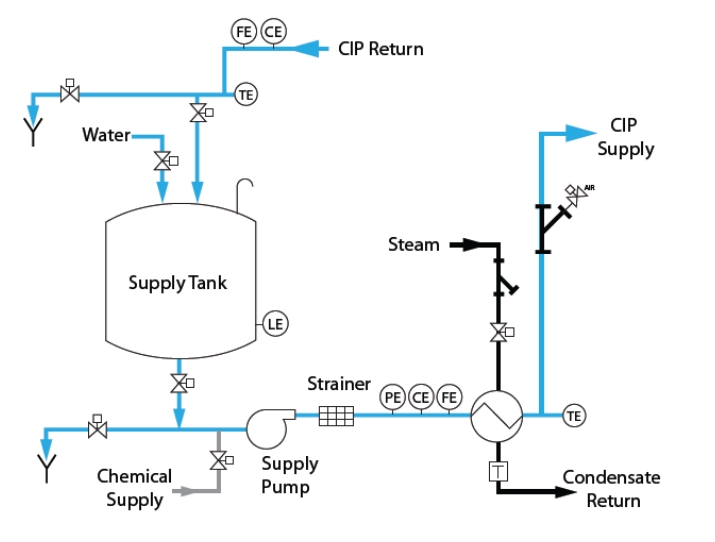
\includegraphics[scale=0.55]{./Resources/cip_example.jpg}
	\captionsetup{justification=centering}
	\caption[Sistema CIP b�sico]{Sistema CIP b�sico. \\Fonte: ROSE e MONTGOMERY (2010)}
	\label{cip_system}
\end{figure}

\subsection{Dimensionamento da parte funcional} 

Com a filosofia de opera��o do sistema mec�nico definida, foi poss�vel realizar o dimensionamento deste sistema. A primeira considera��o a ser feita � que os materiais e m�todos aqui empregados n�o seguem nenhuma norma que permita o uso deste equipamento para fabrica��o de cerveja visando sua comercializa��o --- tal escolha foi feita em fun��o do alto custo de um sistema completamente dentro das normas e tamb�m pelo fato de este ser um trabalho cujo foco � a automa��o e o acesso remoto do sistema, e n�o a comercializa��o de cerveja.

N�o obstante, o material da tubula��o escolhido foi o a�o inoxid�vel AISI304. J� que o volume de l�quido a ser trabalhado � pequeno, menor do que 40 litros, e a press�o de trabalho n�o � maior do que a press�o das bombas escolhidas posteriormente, foi decidido o uso de tubula��o de di�metro de 1/2" (21,34mm de di�metro externo) e espessura da parede no padr�o Schedule 40 (2,77mm de espessura). Embora esta espessura seja superdimensionada para a presente aplica��o, o mec�nico respons�vel pela montagem do sistema a requisitou para que fosse poss�vel fazer rosca sem danificar a integridade dos tubos. As conex�es, seguindo a escolha dos tubos, tamb�m foram de a�o inoxid�vel de 1/2".

As liga��es entre tubos, conex�es e outros componentes do sistema s�o liga��es rosqueadas. Este � um meio de liga��o antigo, por�m de baixo custo, f�cil execu��o e usualmente empregadas em tubula��es de di�metro nominal pequeno, menor do que 4" \cite{ifba}. Para veda��o foi escolhido o Teflon, uma vez que � um material de baixo custo e alta disponibilidade e o padr�o de rosca adotado neste projeto � o BSP, baseado na norma ISO. Cabe salientar que, embora as liga��es rosqueadas sejam permitidas sob certas circunst�ncias na pr�tica, elas s�o relegadas a instala��es de baixa responsabilidade \cite{ifba}.

As panelas foram escolhidas no material de alum�nio, em fun��o do custo proibitivo do a�o inoxid�vel. S�o caldeir�es padr�o utilizados no ramo de hotelaria e restaurantes e dispon�veis em v�rios volumes. As duas panelas utilizadas neste trabalho tem capacidade para 32 litros e di�metro do fundo de 36cm, portanto sua especifica��o no mercado � \textit{caldeir�o de alum�nio n. 36}. Tal volume, 60\% superior ao da produ��o m�xima aconselhada para este sistema, � necess�rio devido ao volume dos gr�os, � quantidade da �gua de lavagem e �s perdas por evapora��o que exigem uso de um volume de �gua inicial superior ao nominal.

O par�metro inicial escolhido para sele��o das v�lvulas solen�ide foi a temperatura m�xima de opera��o, cuja fonte de dados de opera��o � fornecida pelos fabricantes. Em seguida, foi escolhida uma veda��o adequada: os dois tipos mais comums de veda��o com suporte a temperatura de pelo menos 100\si{\degree}C s�o o EPDM e FKM (etileno-propileno-dieno e fluoreto de vinilideno, respectivamente) \cite{danfoss_solenoid}. Estes materiais possuem uma tabela de compatibilidade de fluidos cuja classifica��o pode ser satisfat�ria, boa, duvidosa, insatisfat�ria e desconhecida --- tanto para cerveja quanto para o mosto, ambas as veda��es s�o classificadas como satisfat�rias, embora para �gua a classifica��o do FKM seja somente boa \cite{epdm_fkm}. Por fim, um par�metro que foi verificado antes da escolha final das v�lvulas � a posi��o de opera��o, que varia conforme os modelos do fabricante \cite{danfoss_solenoid}. Com base nos par�metros supracitados, foi decidido usar:

\begin{itemize}
	\item V�lvula solen�ide 1/2" 12V pl�stico uso geral para �gua de resfriamento do trocador de calor.
	\item V�lvula solen�ide Danfoss 1/2" EV210BD 032U3620 para demais v�lvulas.
	\item Solen�ide Danfoss 15W 12VDC 042N7550 para acionamento das v�lvulas Danfoss.
\end{itemize}

Informa��es t�cnicas sobre a v�lvula EV210BD 032U3620 est�o no anexo \ref{Anexo3} e sobre a bobina 042N7550 no anexo \ref{Anexo4}.

As bombas de recircula��o foram escolhidas com base na temperatura de opera��o e grau aliment�cio. Posteriormente, tanto a vaz�o quanto a perda de carga do sistema foram estimadas para verificar se a bomba escolhida era adequada: o modelo Topsflo B08H-12-1006 tem capacidade m�xima de vaz�o de 10l/min e carga expressa em coluna de �gua de 6m. Como a capacidade m�xima do sistema � de 20l e idealmente a temperatura deve subir � taxa de 1\si{\degree}C/min, al�m de que a altura do sistema � menor do que 2m e as perdas de carga n�o decorrentes da gravidade foram consideradas desprez�veis para este caso, foi decidido que a bomba escolhida � adequada ao projeto. No anexo \ref{Anexo5} encontra-se a folha de dados t�cnicos do dispositivo.

Quanto �s conex�es, a figura \ref{conexoes_rascunho} apresenta um diagrama conceitual do sistema, contendo as pe�as necess�rias para a montagem do mesmo:

\begin{figure}[H]
	\centering
	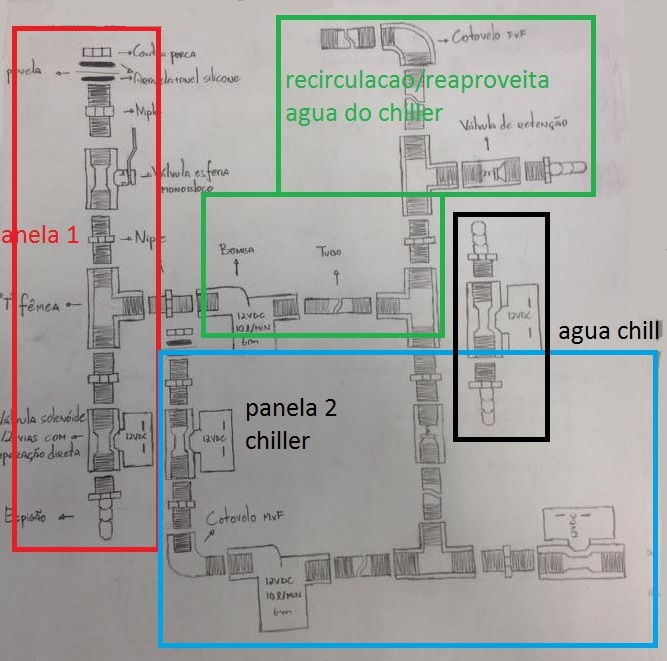
\includegraphics[scale=0.55]{./Resources/conexoes.jpg}
	\captionsetup{justification=centering}
	\caption[Diagrama conceitual das conex�es mec�nicas]{Diagrama conceitual das conex�es mec�nicas}
	\label{conexoes_rascunho}
\end{figure}

\newline

Na figura \ref{mt_cad} � apresentado um diagrama da MT constru�do no software FreeCAD, � qual est�o conectados o resistor de pot�ncia e um niple com veda��o. Tamb�m est�o presentes na figura a v�lvula esfera manual, um \textit{tee} f�mea, uma v�lvula Danfoss EV210B e tr�s niples de conex�o entre estes componentes. O modelo da v�lvula foi obtido a partir do website da Danfoss e importado, enquanto a modelagem dos outros componentes foi desenvolvida na plataforma FreeCAD. Na figura \ref{mt_cad_close} s�o apresentadas em detalhe as conex�es do resistor e do niple � panela e, por isto, a estrutura da mesma foi omitida. Os itens em amarelo s�o contra-porcas, em azul arruelas e, em vermelho an�is de veda��o (\textit{o-rings}).

\begin{figure}[H]
	\centering
	\begin{subfigure}{.46\textwidth}
		\centering
		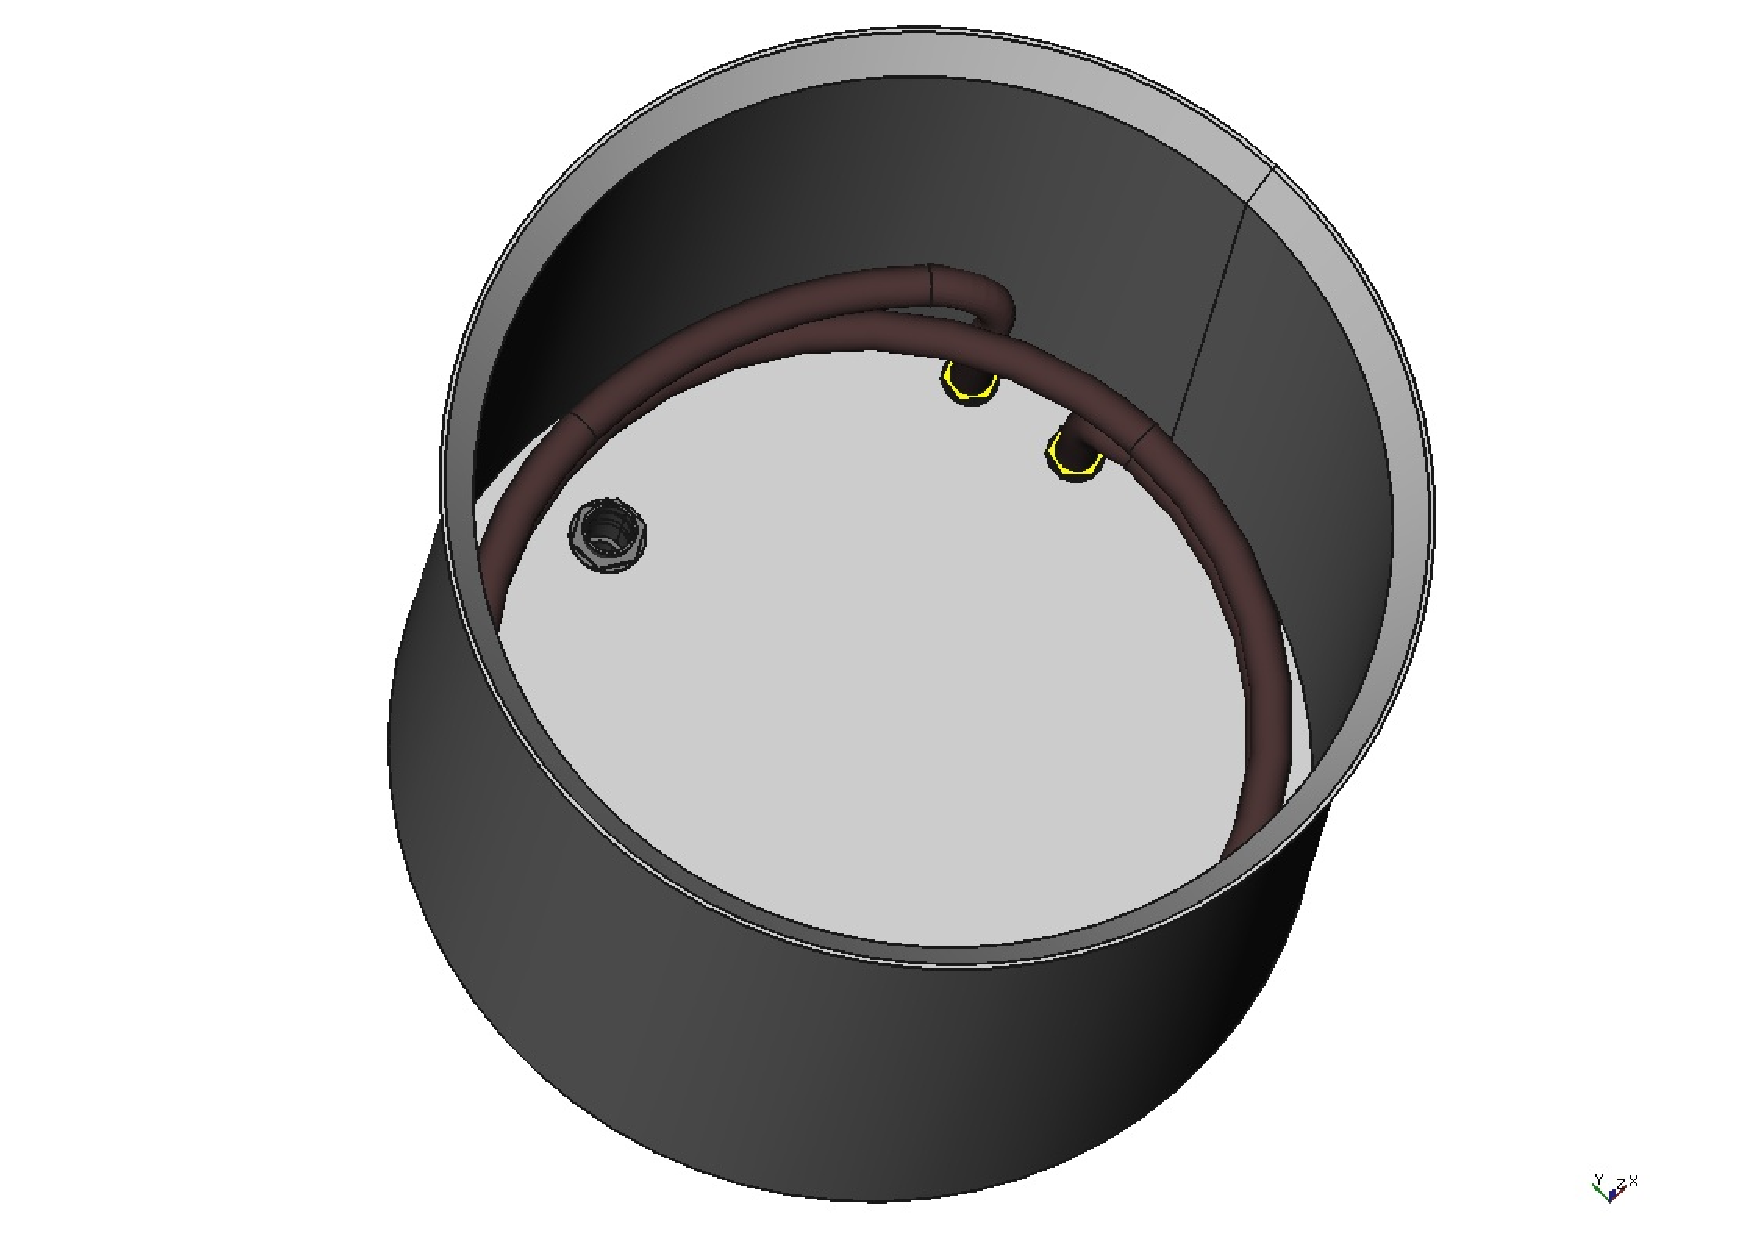
\includegraphics[height=5.5cm]{./Resources/mecsys/mash-tun-top-color.pdf}
		\caption{Vista superior}
		\label{mt_cad:1}
	\end{subfigure}
	\begin{subfigure}{.46\textwidth}
		\centering
		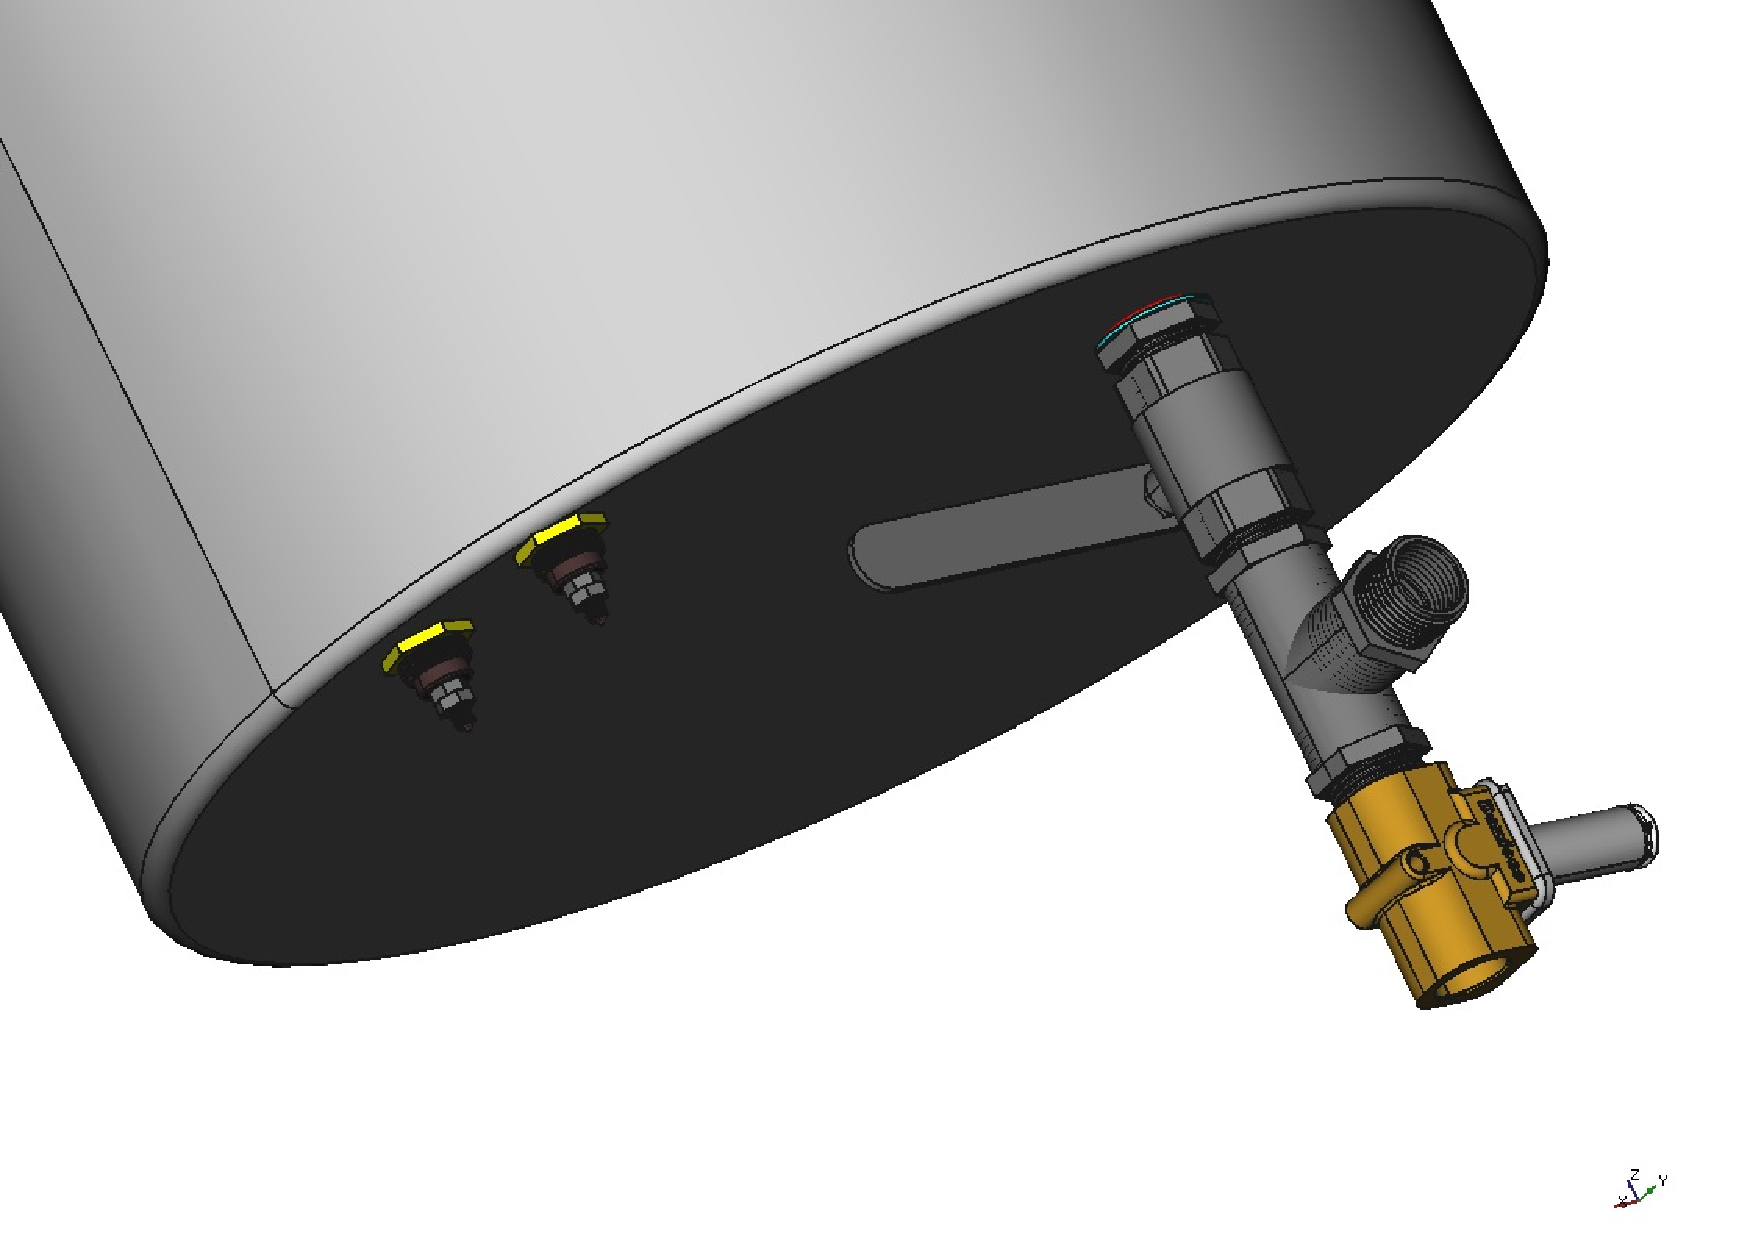
\includegraphics[height=5.5cm]{./Resources/mecsys/mash-tun-bottom-color.pdf}
		\caption{Vista inferior}
		\label{mt_cad:2}
	\end{subfigure}
	\captionsetup{justification=centering}
	\caption[Diagrama da panela de mostura e conex�es]{Diagrama da panela de mostura e conex�es}
	\label{mt_cad}
\end{figure}

\begin{figure}[H]
	\centering
	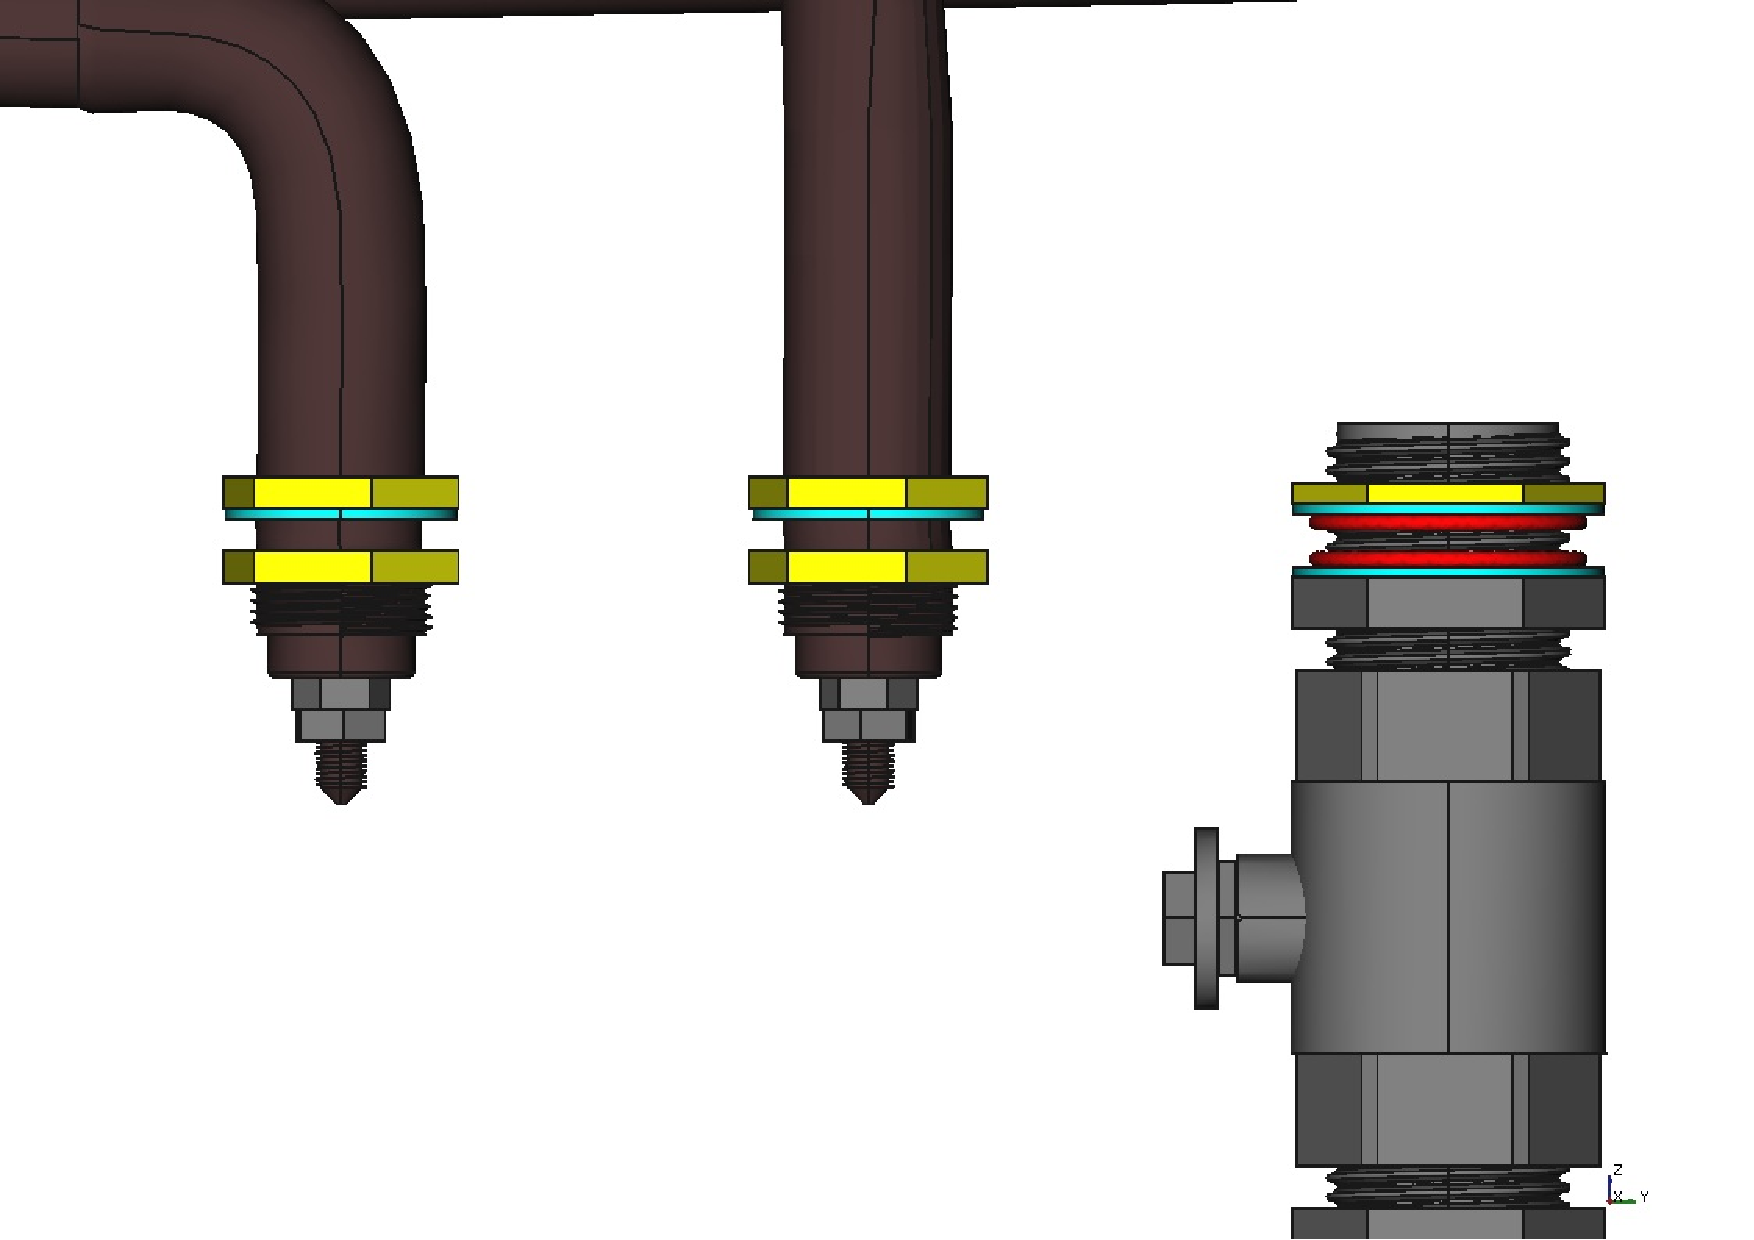
\includegraphics[scale=0.4]{./Resources/mecsys/mash-tun-seal-color.pdf}
	\captionsetup{justification=centering}
	\caption[Detalhes da veda��o da panela de mostura]{Detalhes da veda��o da panela de mostura}
	\label{mt_cad_close}
\end{figure}

\newpage

\subsection{Estrutura met�lica de suporte}

Parte importante do projeto � o dimensionamento da estrutura met�lica de suporte �s panelas, j� que esta � respons�vel n�o somente pelo alojamento do sistema mec�nico como tamb�m pela facilidade de manuten��o. Para defini��o da posi��o das panelas, foram medidas primeiramente as suas alturas e da estrutura de adi��o de l�pulos (que ser� detalhada � parte na se��o \ref{hopbox}) e do \textit{chiller}. Na sequ�ncia, foi estimado um espa�o de manobra entre as duas panelas e uma altura m�nima do ch�o, com base na figura \ref{esboco}. Todas as medidas citadas est�o dispostas na tabela \ref{alturas}.

\begin{center}
	\begin{table}[H]
		\captionsetup{justification=centering}
		\caption[Dimens�es elementos mec�nicos relevantes para o projeto da altura da estrutura met�lica]{Dimens�es elementos mec�nicos relevantes para o projeto da altura da estrutura met�lica}
		\label{alturas}
		\begin{tabular}{ | M{10cm} | M{5cm} |}
			\hline
			\textbf{Descri��o} & \textbf{Altura (cm)} \\ \hline
			Panela BK & 30,0\\ \hline
			Panela MT & 30,0\\ \hline
			\textit{Chiller} & 30,0\\ \hline			
			Estrutura dos l�pulos aberta & 20,0\\ \hline
			V�o livre entre panelas & 20,0\\ \hline
			V�o do \textit{chiller} ao BK & 10,0\\ \hline
			Espa�o entre MT e topo & 10,0\\ \hline
		\end{tabular}
	\end{table}
\end{center}

Somando-se todos os valores da tabela \ref{alturas}, obteve-se que a estrutura met�lica deve ter 1,5m de altura. A largura deve ser de 36,5cm para acomodar as panelas com uma pequena folga e o comprimento escolhido � de 70cm, o que permite alinhar as panelas de maneira n�o conc�ntrica, conforme abordado na se��o \ref{estmec} --- este valor � suficiente, j� que o di�metro somado das duas panelas � de 72cm e � preciso que exista uma intersec��o para permitir o escoamento por gravidade da MT ao BK. Na figura \ref{estmec_cad} � apresentado o projeto da estrutura j� com as prateleiras para acomodar as panelas. Note-se que foram escolhidas cantoneiras de 2" x 1/8" para a constru��o deste equipamento.

\begin{figure}[H]
	\centering
	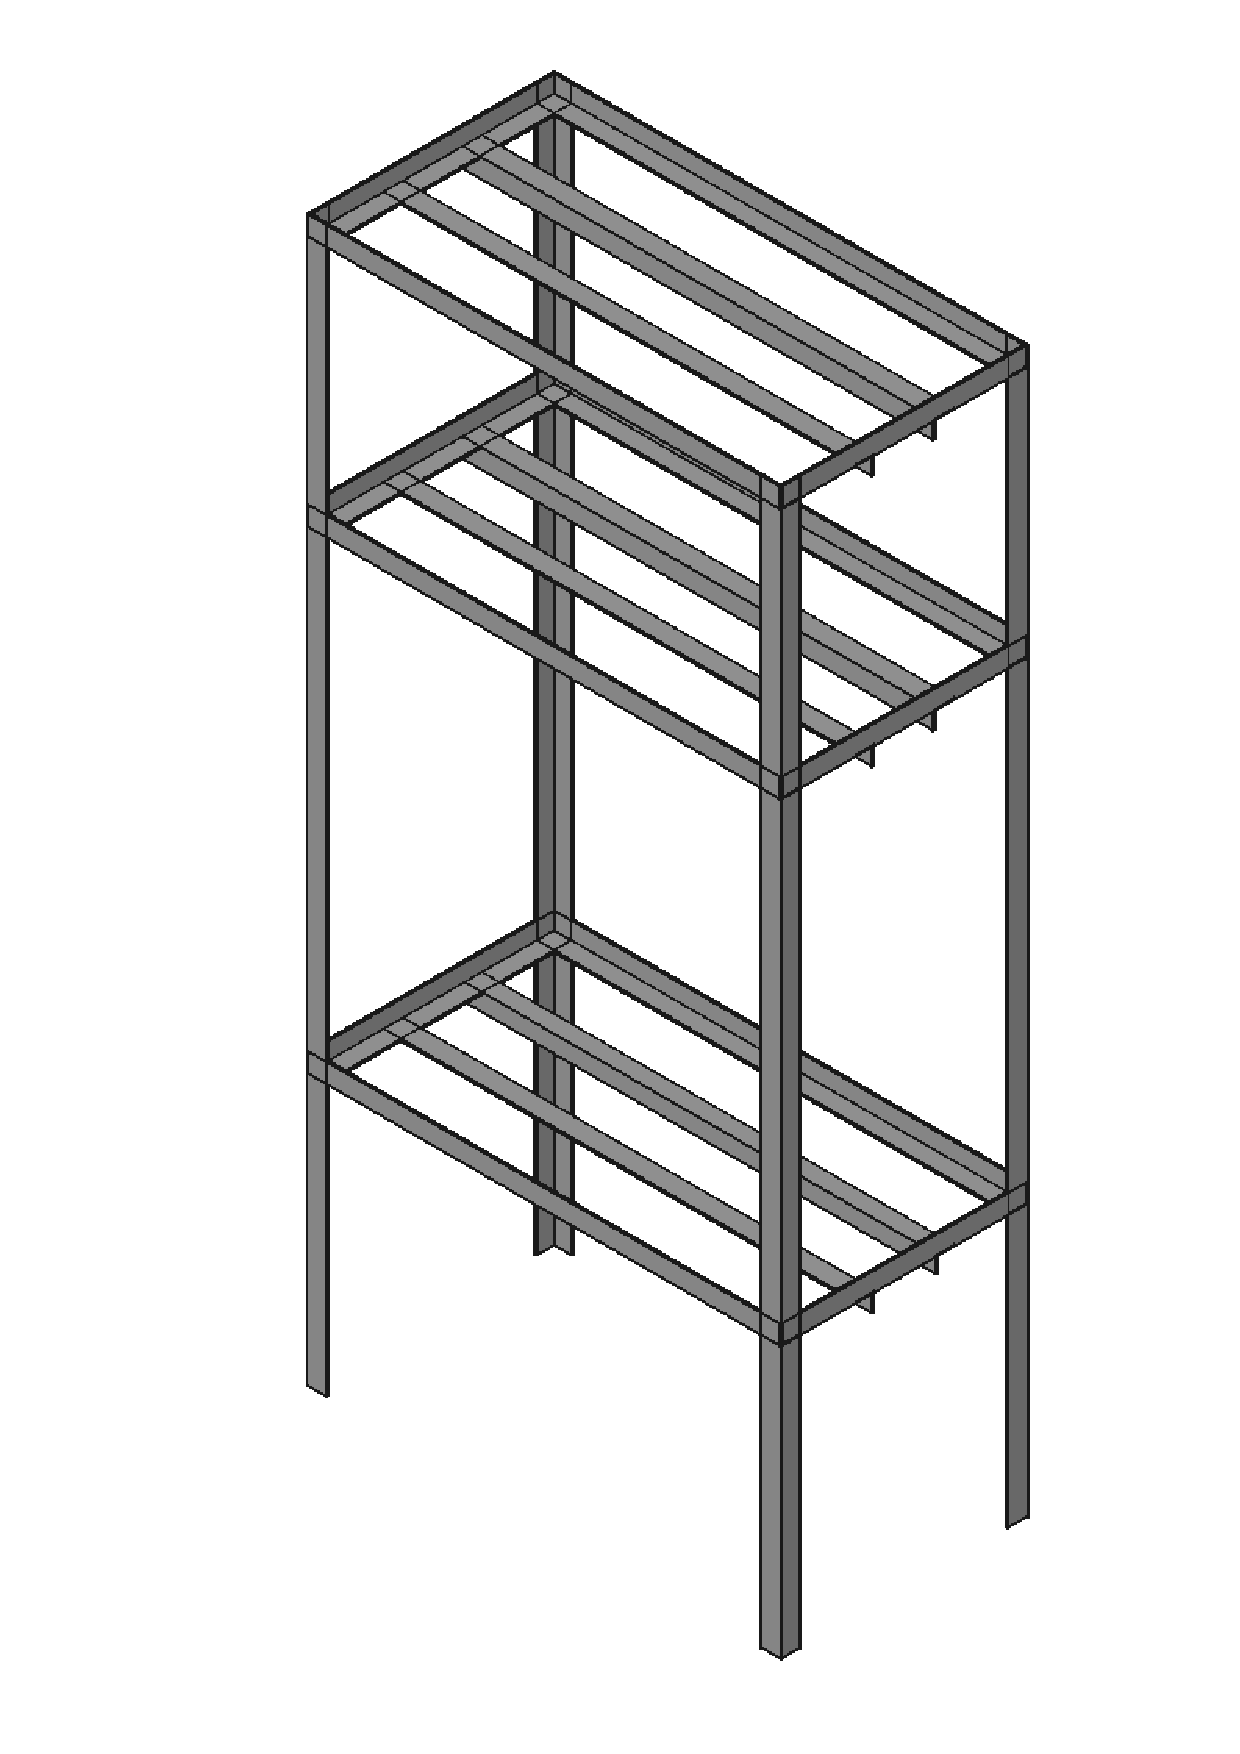
\includegraphics[scale=0.35]{./Resources/mecsys/estmec-freecad.pdf}
	\captionsetup{justification=centering}
	\caption[Projeto da estrutura met�lica]{Projeto da estrutura met�lica}
	\label{estmec_cad}
\end{figure}


%%%%%%%%%%%%%%%%%%%%%%%%%%%%%%%%%%%%%%%%%%%%%%%%%%%%%%%%%%%%%%%%%%%%%%%%%%

\section{Estrutura de adi��o de l�pulos}
\label{hopbox}
Devido � necessidade de adicionar l�pulos � receita em propor��es e tempos predefinidos, foi necess�rio o projeto de uma estrutura autom�tica de adi��o de l�pulos. Em fun��o das in�meras possibilidades de combina��es de l�pulos e temporiza��es, a escolha natural do projeto foi uma estrutura que permita esta flexibilidade --- uma caixa com oito compartimentos separados para adi��o sequencial destes insumos. Com base em um pacote de l�pulos em \textit{pellets} de 50g, estimou-se que seu volume � de $160cm^3$ e, sabendo-se que uma receita de 20l dificilmente utiliza uma quantidade maior do que 400g de l�pulos, a decis�o tomada foi a de que cada um dos 8 compartimentos deveria ter os $160cm^3$ necess�rios para acomodar 50g. Para confirmar que 400g � uma quantidade razo�vel, foi seguido o c�lculo de IBU de \cite{palmer}, detalhado no ap�ndice \ref{Ap�ndice C}.

Fixando a altura do compartimento em 10,0cm foram escolhidos valores de comprimento e largura de 16,0cm e 8,0cm respectivamente, assumindo inicialmente que as paredes das divis�rias tem espessura desprez�vel. A equa��o para volume de um prisma e a escolha das dimens�es s�o demonstradas em \ref{eq_hop_vini}:

\begin{subequations}
	\label{eq_hop_vini}
	\begin{align}
		V &= l\cdot w\cdot h = V_{50g}\cdot 8 \\
		&= l\cdot w\cdot 10 = 160\cdot 8 \nonumber \\
		l\cdot w\cdot &= 128, fixando \quad l = 16cm \quad \therefore \nonumber \\
		w &= 128/16 = 8cm \quad e \\
		w_{compartimento} &= l/8 = 16/8 = 2cm
	\end{align}
\end{subequations}

Posteriormente aos c�lculos de \ref{eq_hop_vini}, durante o projeto no software FreeCAD, observou-se que a assump��o de espessura desprez�vel � falsa e um retrabalho nas medidas do compartimento levou �s dimens�es externas finais de 18,0cm x 8,4cm x 10,0cm; as paredes externas tendo espessura de 3,0mm e as internas de 2,0mm. A figura \ref{caixa_cinza} esbo�a as dimens�es externas da caixa e a figura \ref{corpo_hopbox} apresenta o corpo da estrutura.

\begin{figure}[H]
	\centering
	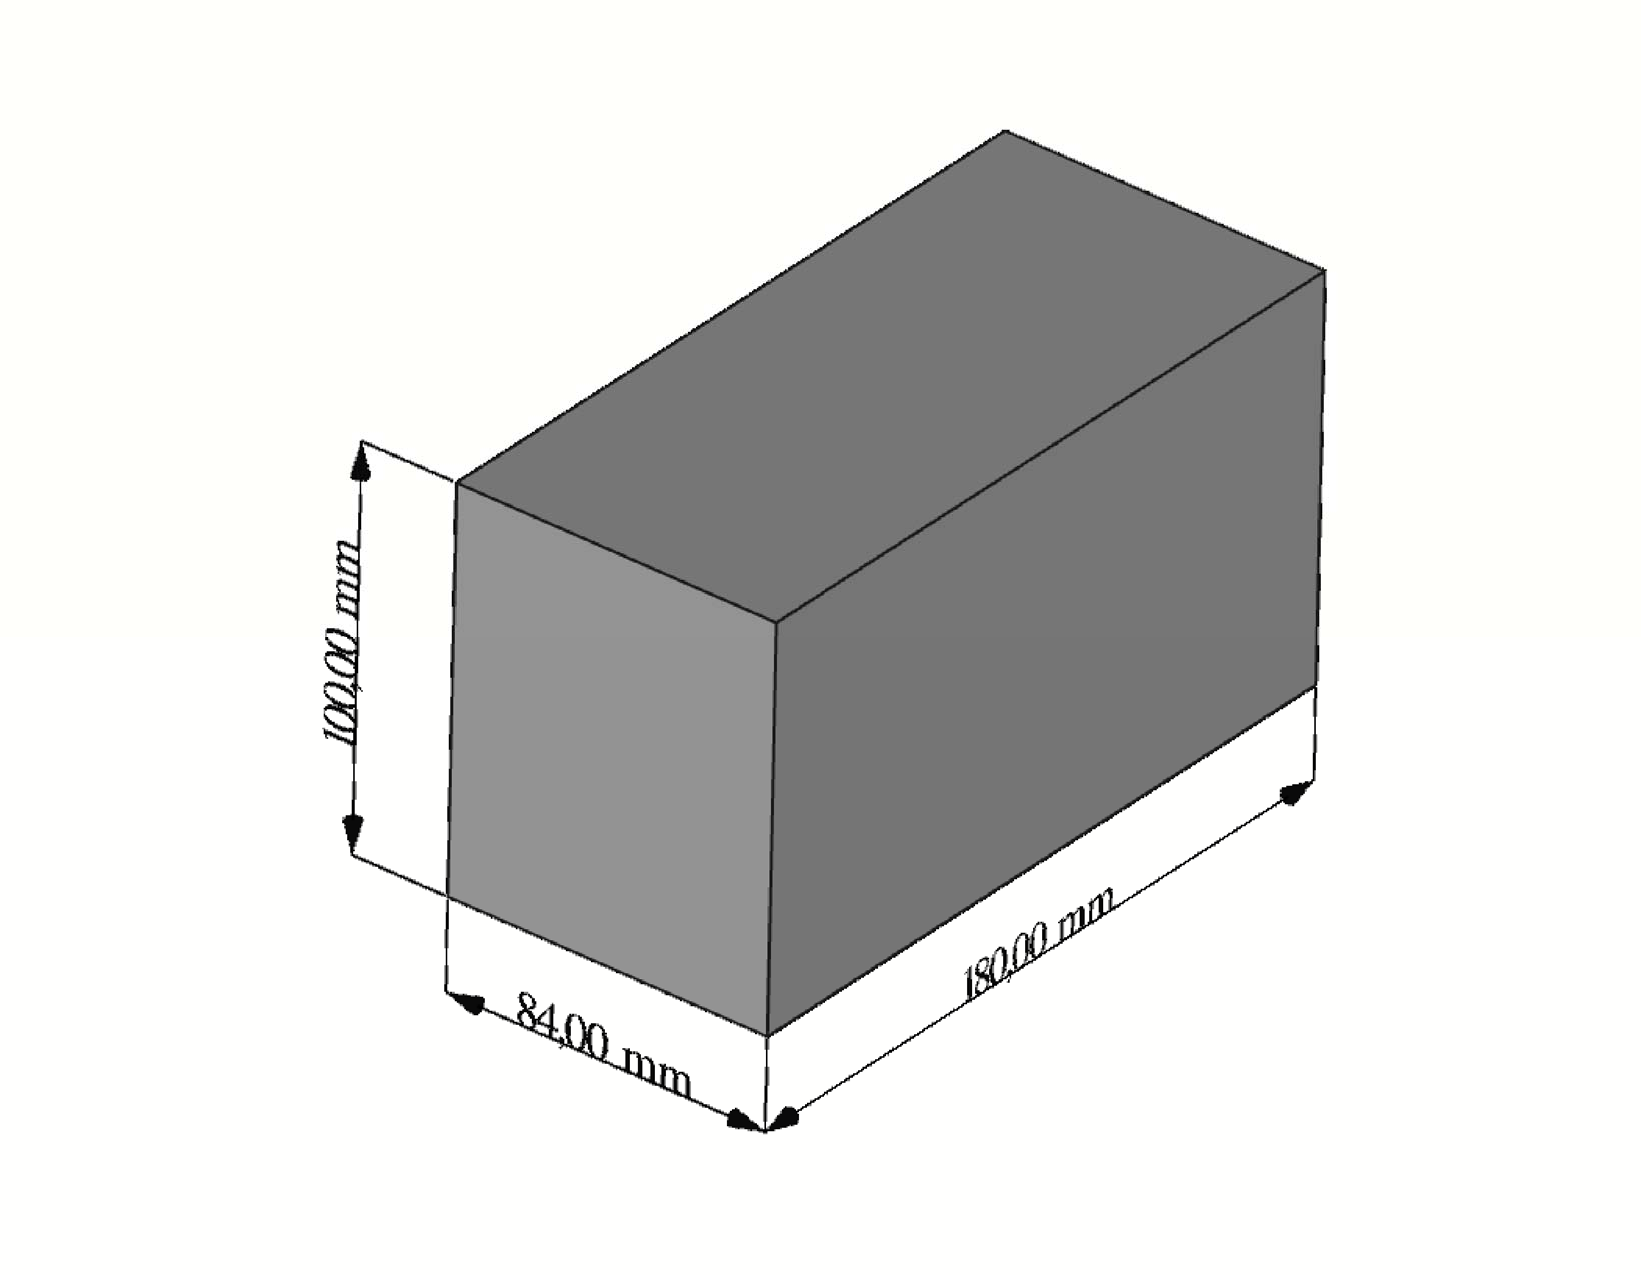
\includegraphics[scale=0.35]{./Resources/estLup/caixa_lupulos(1).pdf}
	\captionsetup{justification=centering}
	\caption[Dimens�es da estrutura de adi��o de l�pulos]{Dimens�es da estrutura de adi��o de l�pulos}
	\label{caixa_cinza}
\end{figure}

\begin{figure}[H]
	\centering
	\begin{subfigure}{.46\textwidth}
		\centering
		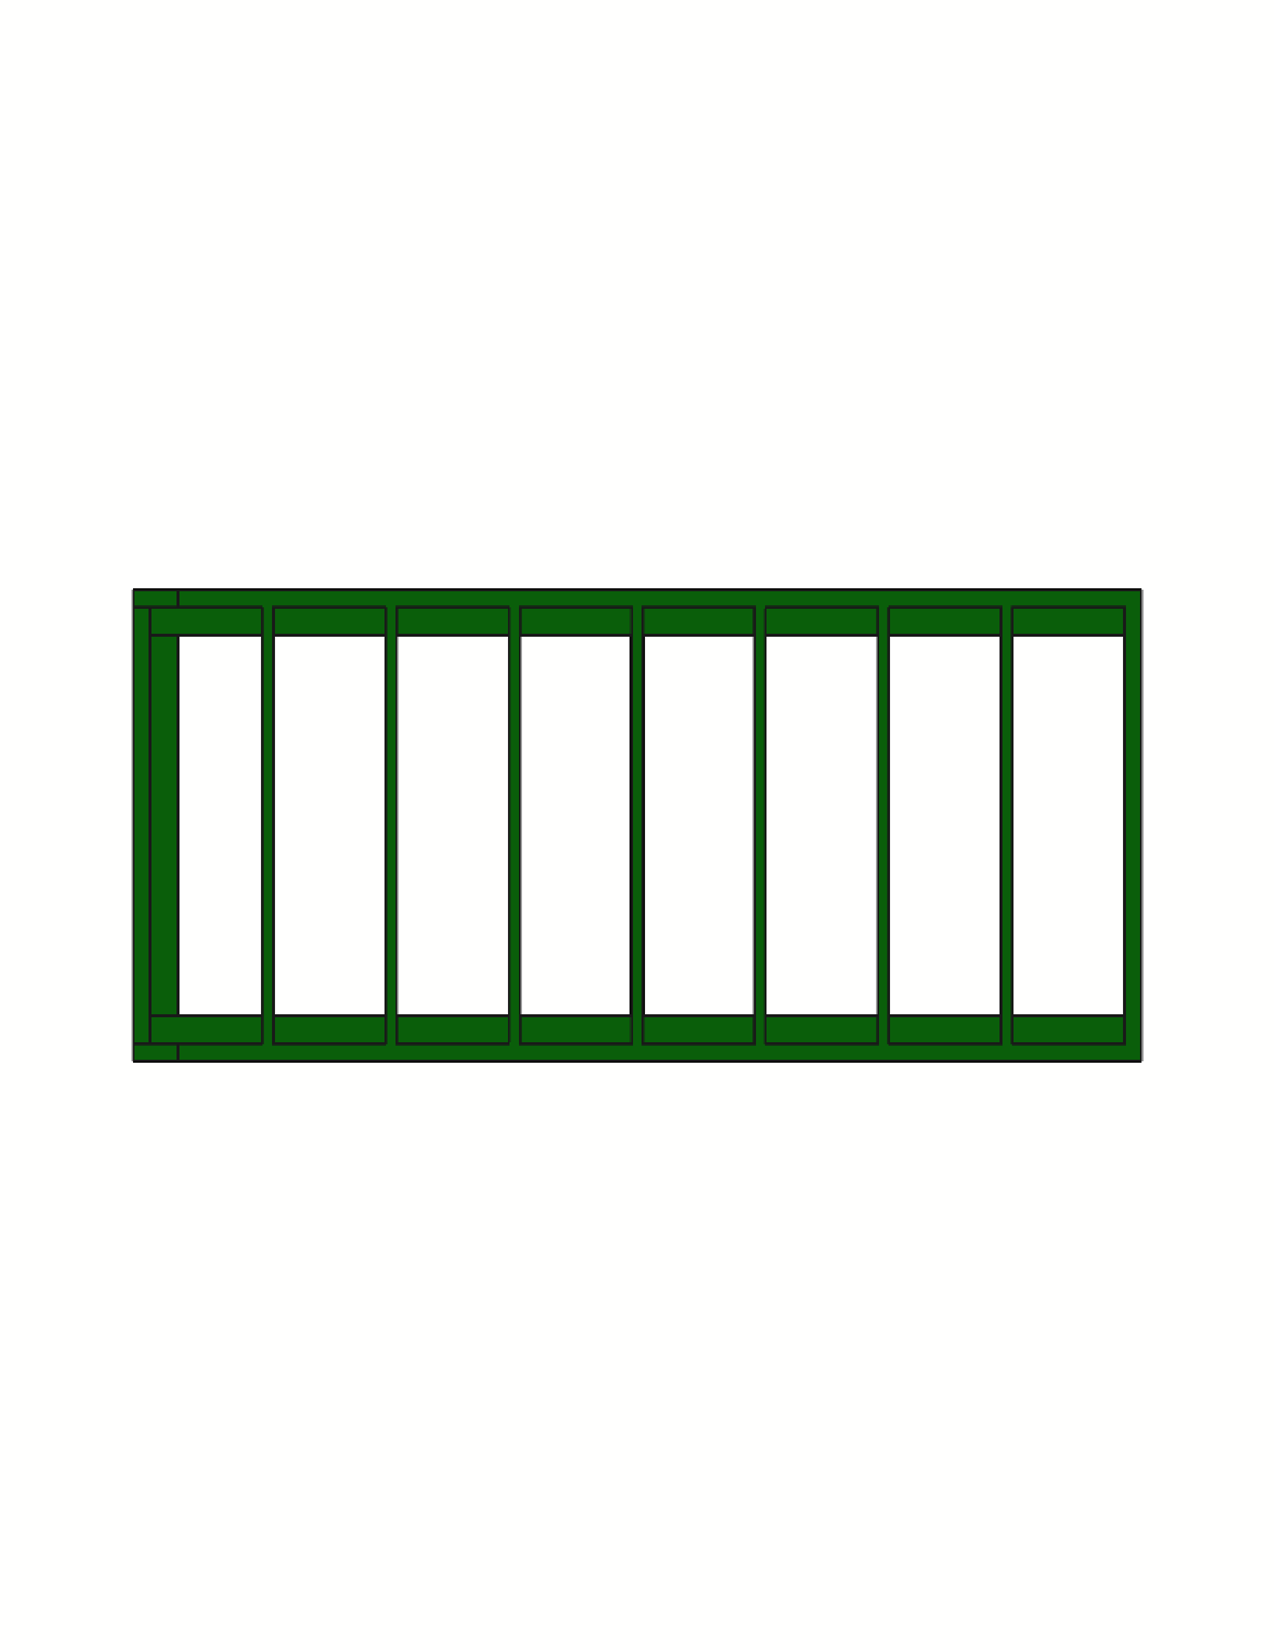
\includegraphics[height=7.5cm]{./Resources/estLup/caixa_lupulos(2).pdf}
		\caption{Vista superior}
		\label{corpo_hopbox:1}
	\end{subfigure}
	\begin{subfigure}{.46\textwidth}
		\centering
		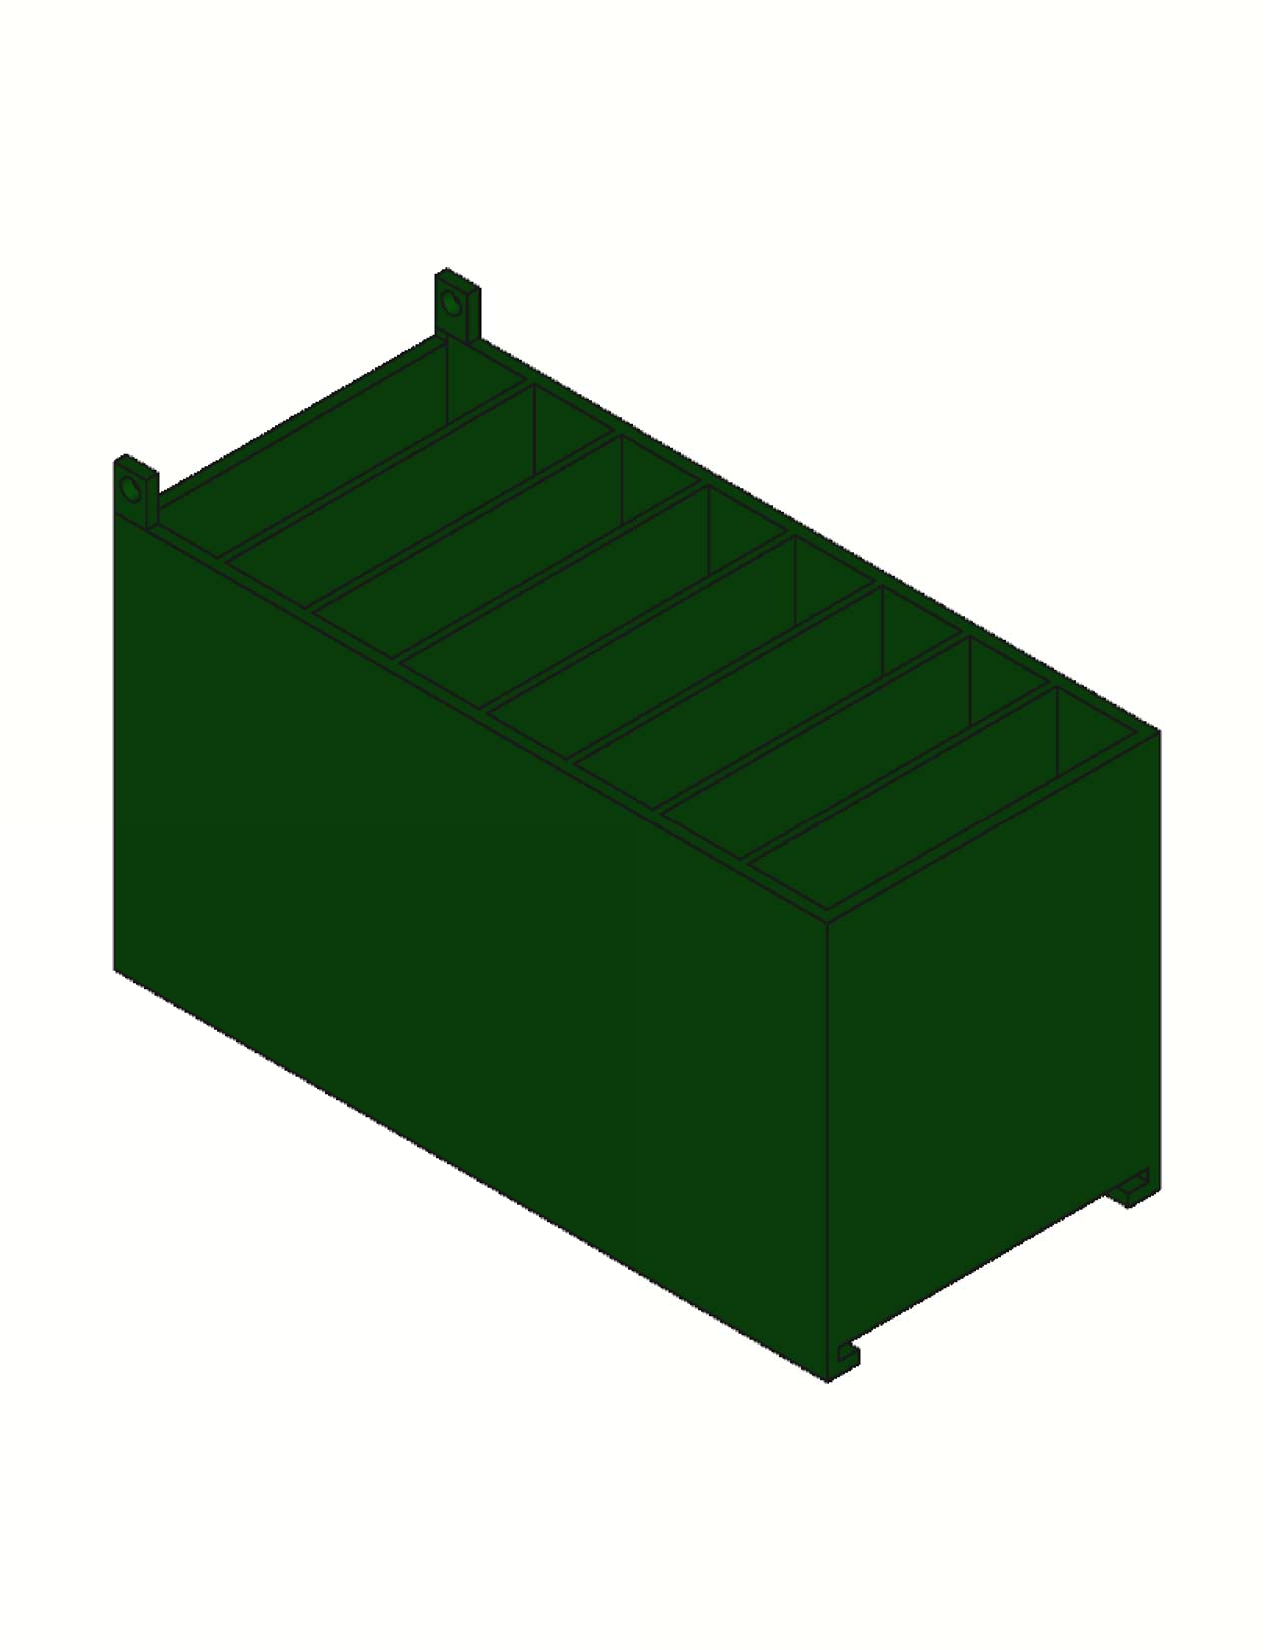
\includegraphics[height=7.5cm]{./Resources/estLup/caixa_lupulos(3).pdf}
		\caption{Vista axiom�trica}
		\label{corpo_hopbox:2}
	\end{subfigure}
	\captionsetup{justification=centering}
	\caption[Corpo da estrutura de adi��o de l�pulos]{Corpo da estrutura de adi��o de l�pulos}
	\label{corpo_hopbox}
\end{figure}

Foram projetadas duas portinholas: uma na face superior da caixa, para reabastecimento manual dos l�pulos, com uma al�a e fixada na caixa por dois pinos, de modo que a abertura desta tampa � um movimento de rota��o e; uma na face inferior, para adi��o autom�tica, de correr, de modo que a abertura � um movimento de transla��o; ambas est�o ilustradas na figura \ref{tampas_hopbox}.

\begin{figure}[H]
	\centering
	\begin{subfigure}{.46\textwidth}
		\centering
		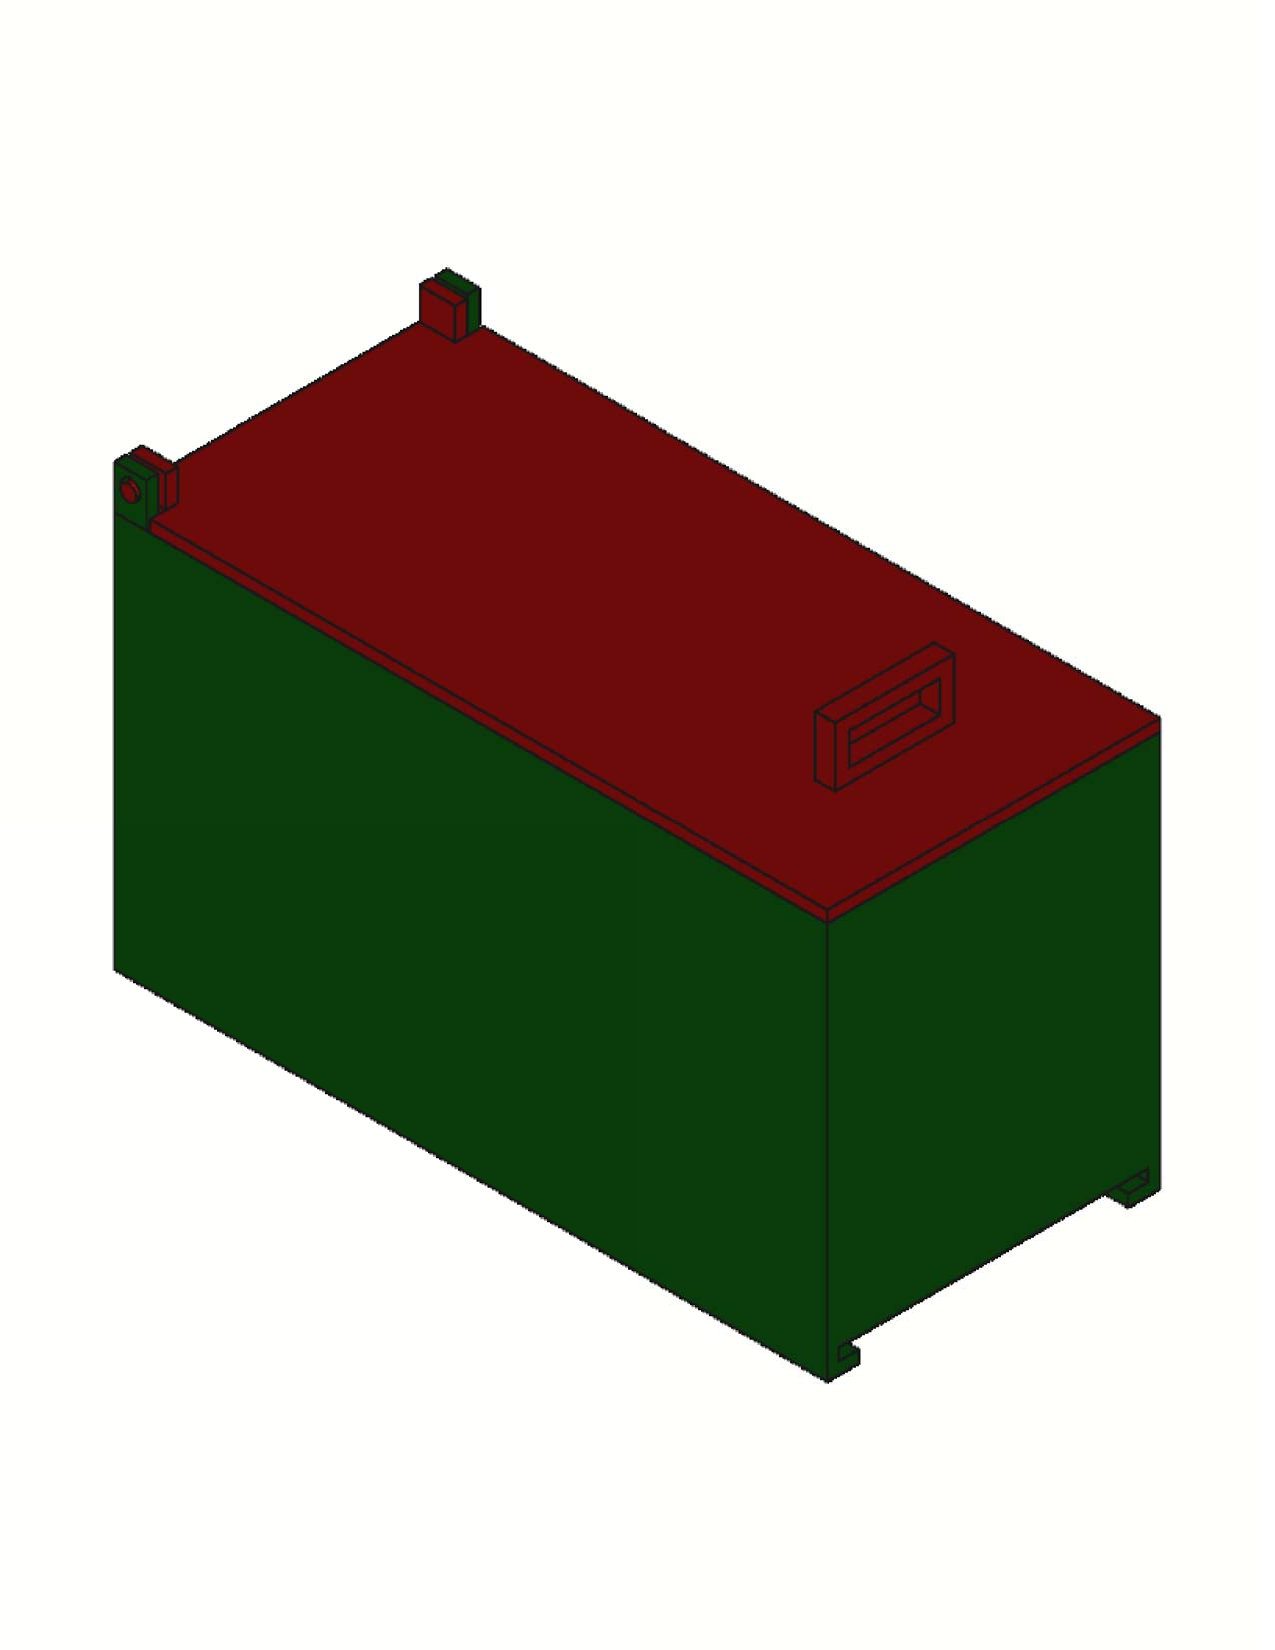
\includegraphics[height=7.5cm]{./Resources/estLup/caixa_lupulos(4).pdf}
		\caption{Tampa manual para reabastecimento}
		\label{tampas_hopbox:1}
	\end{subfigure}
	\begin{subfigure}{.46\textwidth}
		\centering
		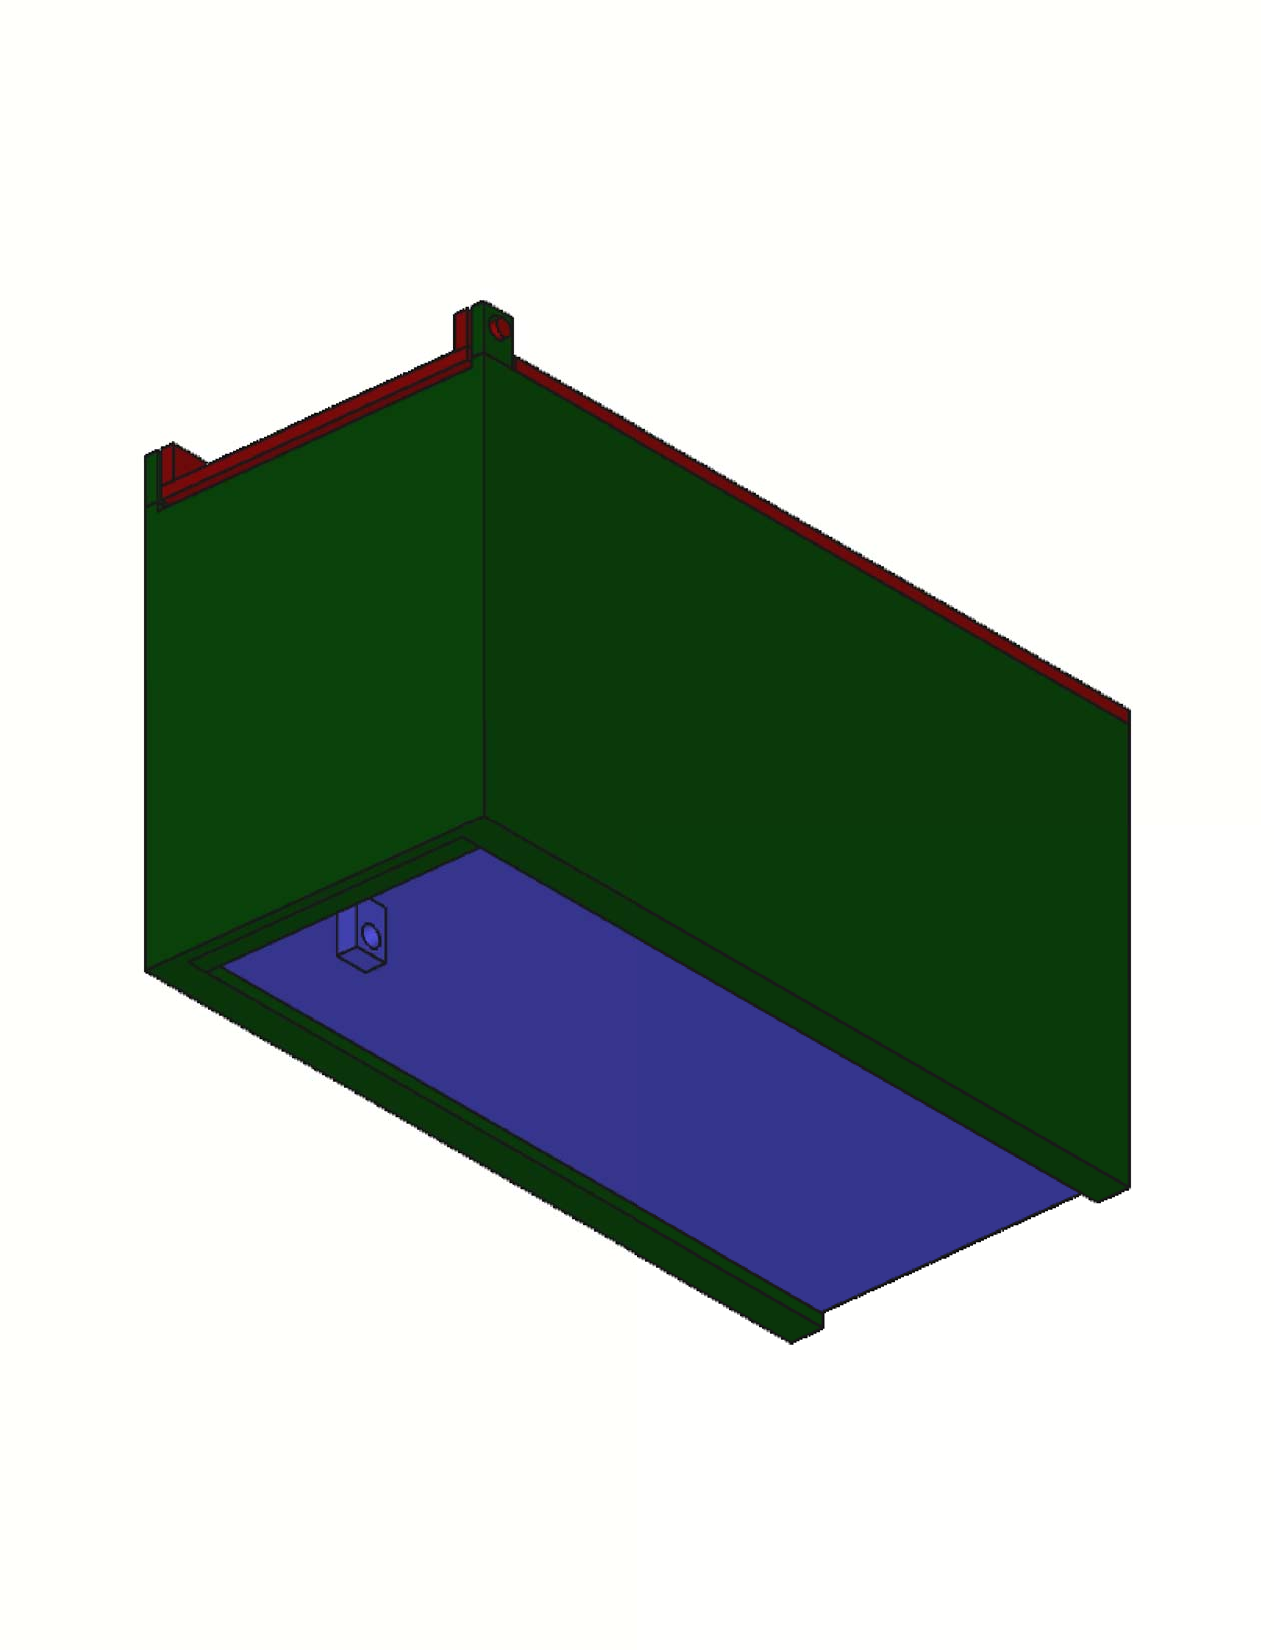
\includegraphics[height=7.5cm]{./Resources/estLup/caixa_lupulos(5).pdf}
		\caption{Tampa para adi��o autom�tica dos l�pulos}
		\label{tampas_hopbox:2}
	\end{subfigure}
	\captionsetup{justification=centering}
	\caption[Tampas da estrutura de adi��o de l�pulos]{Tampas da estrutura de adi��o de l�pulos}
	\label{tampas_hopbox}
\end{figure}

Duas varetas de comprimento $l_1$ e $l_2$ s�o ligadas ao encaixa da tampa de correr, representada em azul na figura \ref{tampas_hopbox:2}, e a elas � acoplado um servo-motor cujo �ngulo de opera��o $\theta$ define a abertura --- ou deslocamento --- da tampa, definido por $d$. A figura \ref{varetas} esquematiza as liga��es.

\begin{figure}[H]
	\centering
	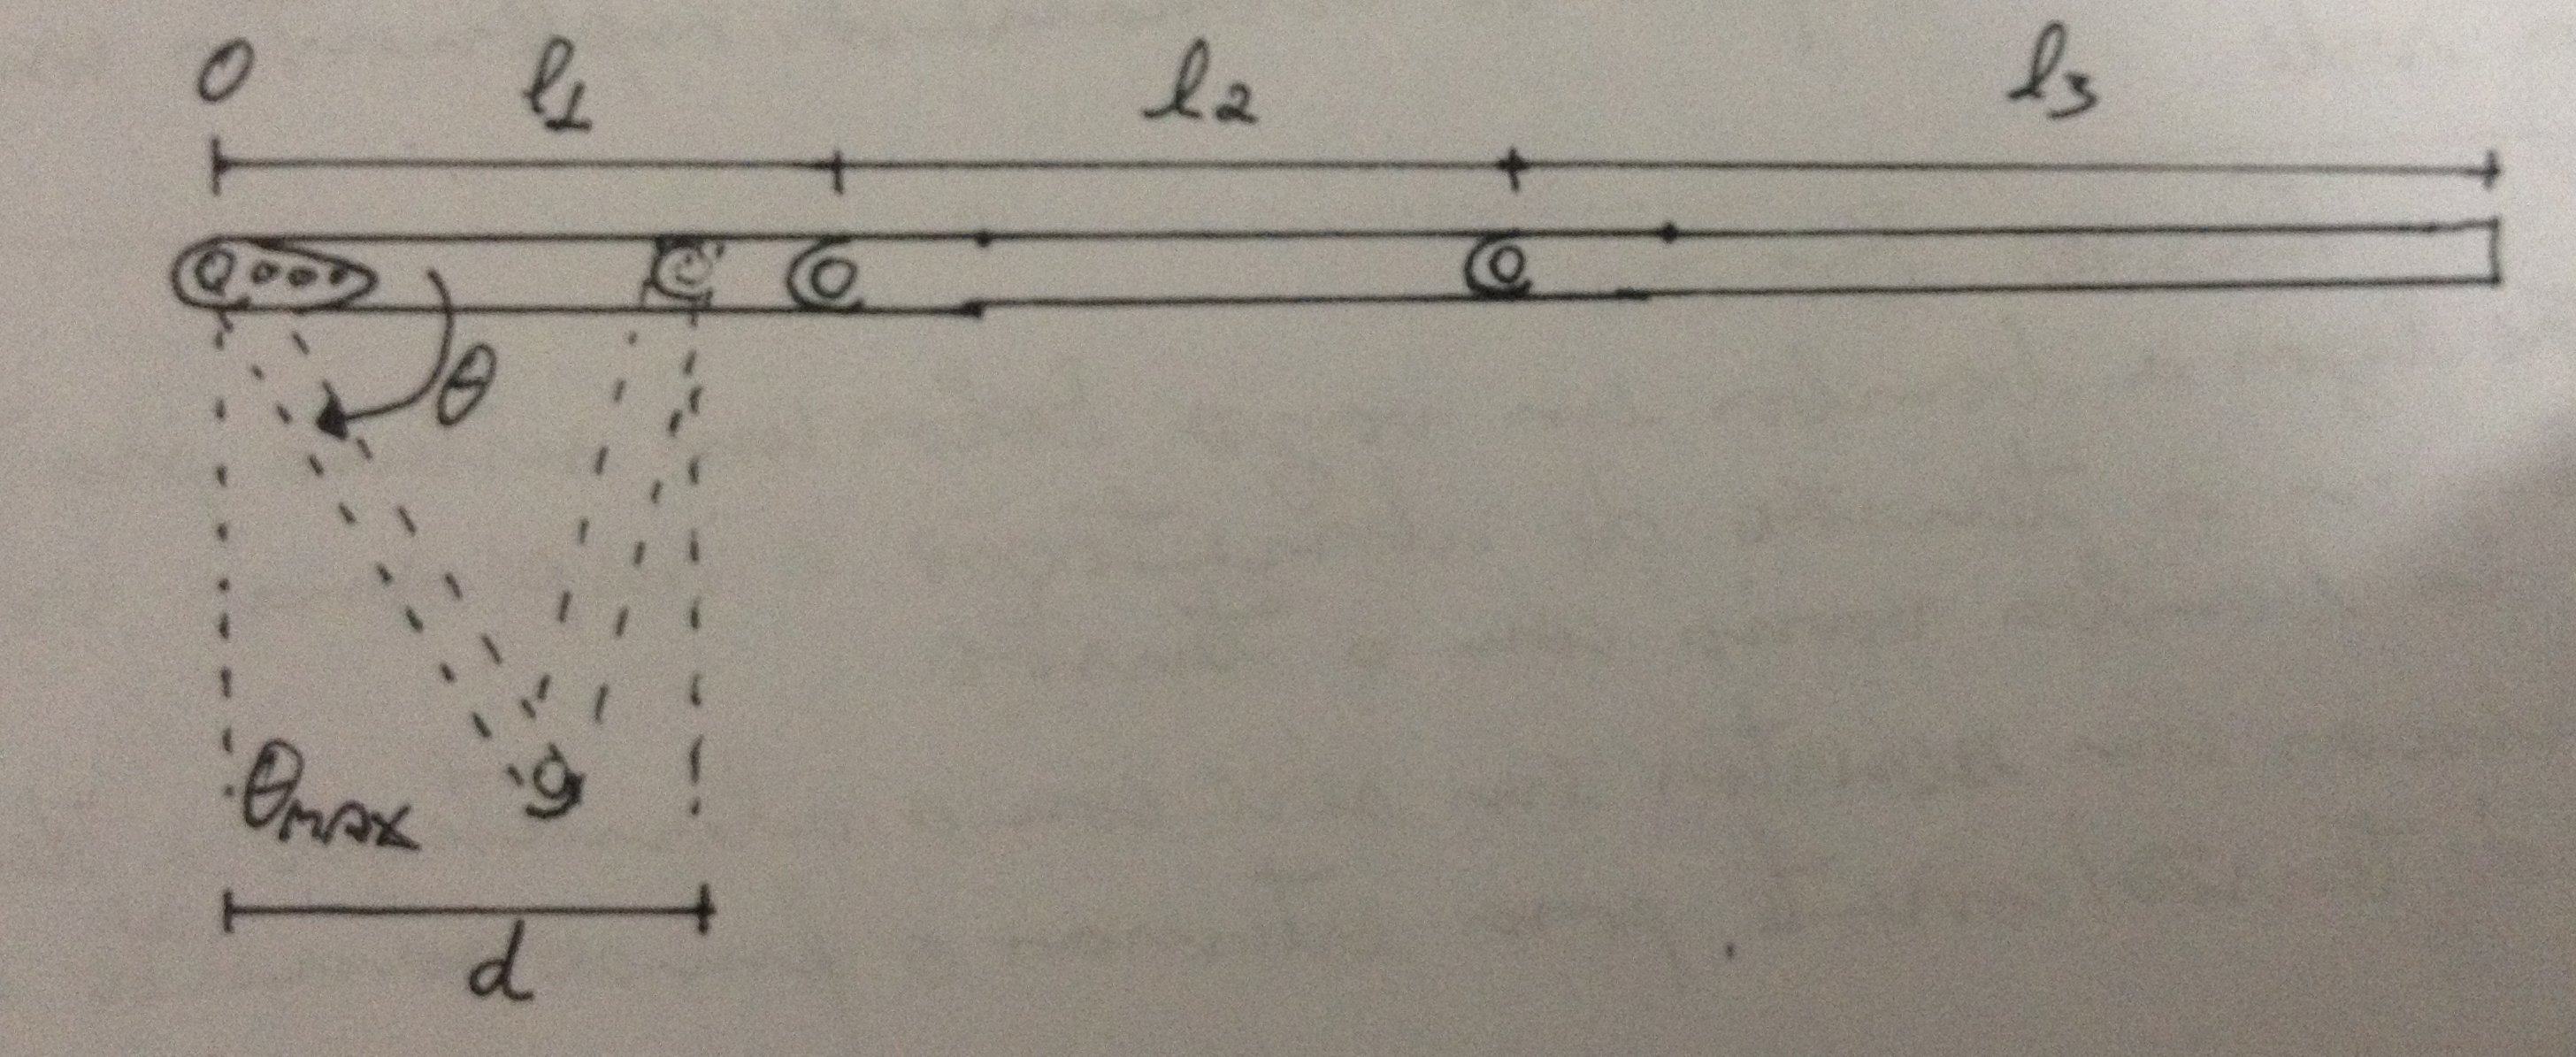
\includegraphics[scale=0.1]{./Resources/estLup/esquema-varetas.jpg}
	\captionsetup{justification=centering}
	\caption[Esquema de liga��o das varetas � tampa de correr]{Esquema de liga��o das varetas � tampa de correr}
	\label{varetas}
\end{figure}

Sendo o comprimento da tampa igual a $l_3$, a condi��o em \ref{eq_varetas} deve ser satisfeita para que a excurs�o m�xima de abertura da caixa possa ser atingida. � poss�vel demonstrar com o aux�lio da Lei dos Cossenos, em \ref{eq_cossenos} que $l_1 = l_2 = l$ para que a m�nima abertura da caixa possa ser atingida.

\begin{align}
	\label{eq_varetas}
	l_1 + l_2 \geq l_3
\end{align}

\begin{align}
	\label{eq_cossenos}
	&l_2^2 = d^2 + l_1^2 - 2dl_1\cdot cos(\theta) \\
	&se \quad \theta = 90\si{\degree} \rightarrow d = 0 \therefore \nonumber\\
	\label{res_cossenos}
	&l_2^2 = l_1^2 \rightarrow l_2 = l_1 = l
\end{align}

A taxa m�xima de deslocamento em fun��o do �ngulo do servo motor � expressa em \ref{eq_desl}:

\begin{align}
	\label{eq_desl}
	\frac{dl_3}{d\theta} = \frac{2l}{90\si{\degree}}
\end{align}

Entretanto, quanto maior o valor desta taxa, menor � a resolu��o de abertura da caixa, portanto obtem-se que o menor valor poss�vel de $l$, a partir de \ref{eq_varetas} � $l = l_3/2$. Assim sendo, a taxa de deslocamento calculada a partir de \ref{eq_desl} � de $2mm/\si{\degree}$.

Embora o valor te�rico de $\theta$ seja $90\si{\degree}$, na pr�tica, devido ao encaixe entre tampa e vareta n�o ser na extremidade, este valor � reduzido. Tal fato n�o deve ser negligenciado, uma vez que isto pode for�ar a opera��o do servo-motor. Sabe-se pelo projeto executado no FreeCAD que a dist�ncia da borda ao encaixe da tampa � de 2,3cm portanto, com o aux�lio da Lei dos Cossenos, obt�m-se que $\theta_{max} = 82\si{\degree}$. Quanto ao valor m�nimo n�o h� preocupa��o , j� que a abertura da caixa ter� uma excurs�o reduzida em 2,3cm com rela��o ao seu comprimento. As varetas n�o foram calculadas novamente pois julgou-se uma boa pr�tica essa redu��o, que evita que a tampa caia da caixa quando em m�xima excurs�o. A figura \ref{completa_hopbox} apresenta o esquema completo de constru��o da estrutura de adi��o de l�pulos.

\begin{figure}[H]
	\centering
	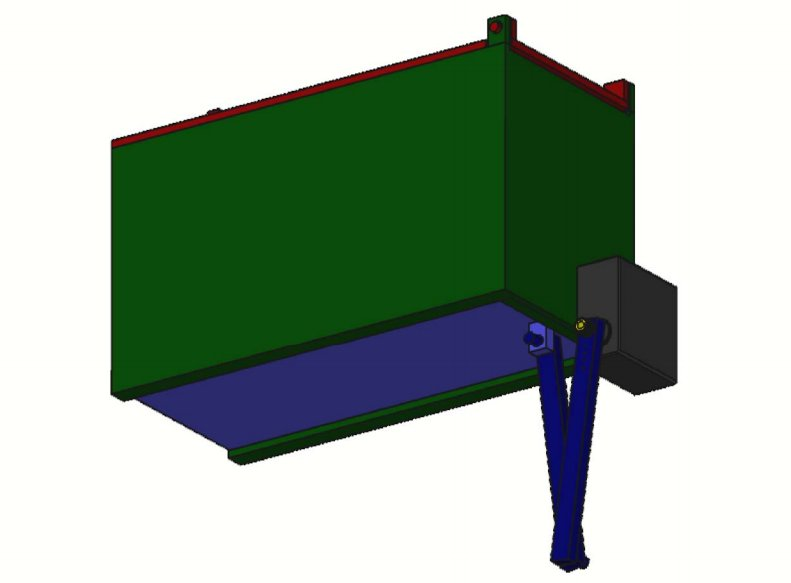
\includegraphics[scale=0.25]{./Resources/estLup/final.jpg}
	\captionsetup{justification=centering}
	\caption[Estrutura de adi��o de l�pulos]{Estrutura de adi��o de l�pulos}
	\label{completa_hopbox}
\end{figure}


%%%%%%%%%%%%%%%%%%%%%%%%%%%%%%%%%%%%%%%%%%%%%%%%%%%%%%%%%%%%%%%%%%%%%%%%%%

%\section{Configura��o da BeagleBone Black}
%O primeiro passo para o desenvolvimento do projeto foi a configura��o da BeagleBone Black, que � o cora��o deste sistema. Para tal, foi escolhido o procedimento de gravar a distribui��o Debian pr�-compilada do sistema operacional Linux na mem�ria de armazenamento eMMC de 4GB da placa. Esta distribui��o foi escolhida em fun��o da facilidade de obten��o de suporte em f�runs da internet, artigos e livros, dentre outros, al�m de ser o SO oficial da BBB \cite{bbb_debian}.

NOTA: Na ocasi�o da realiza��o deste procedimento, havia uma diferencia��o entre a imagem fornecida para uso diretamente a partir do cart�o \si{\micro}SD e a imagem para grava��o no eMMC, por�m agora o procedimento adotado pela funda��o BeagleBoard.org � fornecer somente uma imagem pronta para uso diretamente do cart�o \si{\micro}SD e, no caso de o usu�rio decidir gravar a distribui��o no eMMC, o arquivo uEnv.txt na parti��o de \textit{boot} do cart�o \si{\micro}SD deve ser editado conforme instru��es antes de ser inserido na BBB.

Tanto a �ltima vers�o est�vel do Debian para BBB (v. 7.9), conhecida como \textit{Wheezy} e a �ltima vers�o em desenvolvimento (v. 8.2), conhecida como \textit{Jessie}, quanto a vers�o utilizada neste projeto (v. 7.5) podem ser obtidas a partir do site oficial da BBB \cite{bbb_images}, conforme ilustrado na figura \ref{debian_images}. A instala��o da vers�o 7.5 se resume a:

\begin{enumerate}
	\item Baixar a imagem Debian 7.5 para eMMC do site \url{beagleboard.org/latest-images}
	\item Descomprimir a imagem
	\item Gravar a imagem em um cart�o \si{\micro}SD formatado (n�o basta copiar, � preciso utilizar um software que grave a imagem corretamente. Neste caso foi utilizado o \textit{Win32 Disk Imager})
	\item Inserir o cart�o \si{\micro}SD na BBB desligada
	\item Pressionar o bot�o de boot e energizar a placa com ele ainda pressionado
	\item Esperar um dos leds de status acender antes de largar o bot�o
	\item Esperar os 4 leds de status ficarem continuamente acesos (durante o processo de grava��o eles trabalhar�o de maneira intermitente)
	\item Desenergizar a BBB e retirar o cart�o \si{\micro}SD
\end{enumerate}
 
 \newpage
 
\begin{figure}[H]
	\centering
	\fbox{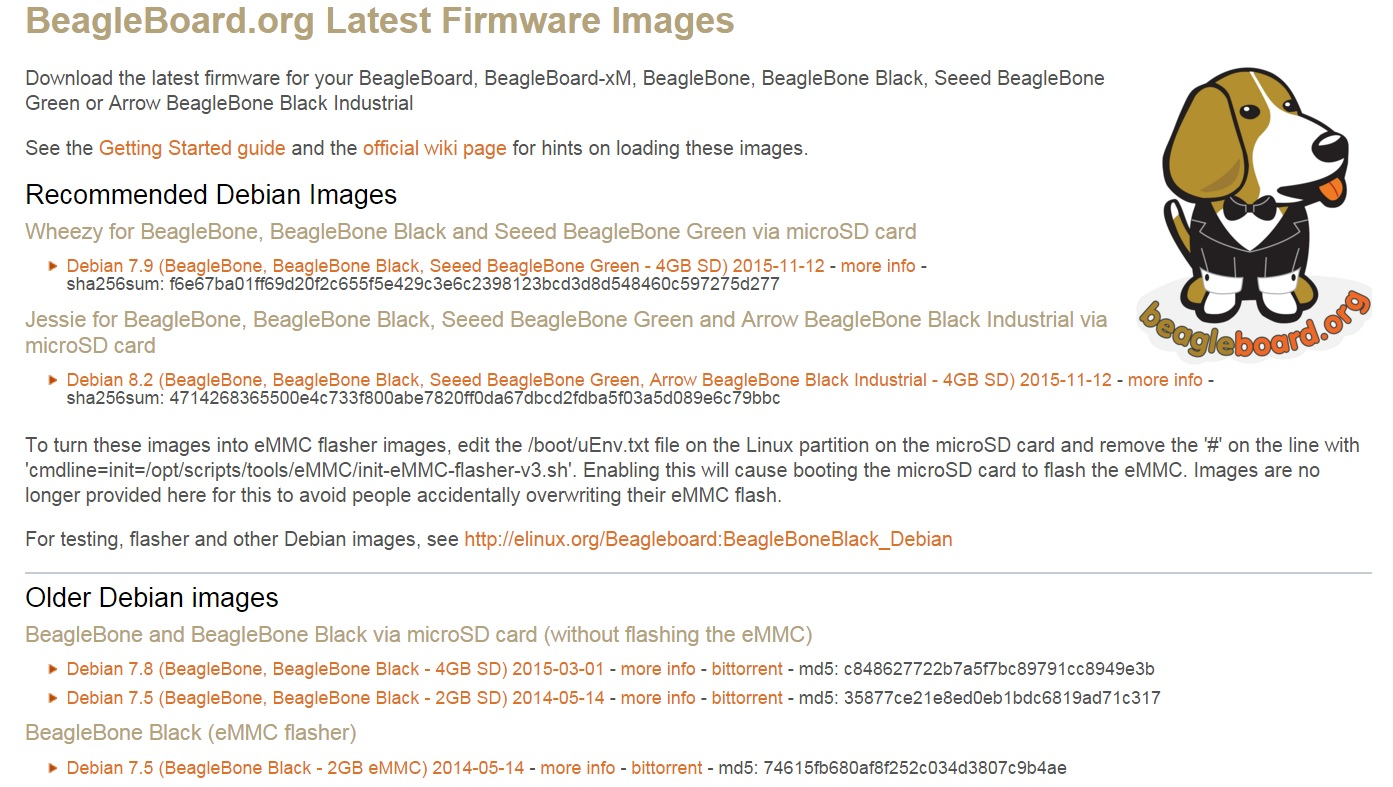
\includegraphics[scale=0.30]{./Resources/debian-latest.jpg}}
	\captionsetup{justification=centering}
	\caption[�ltimas imagens pr�-compiladas dispon�veis para a BBB]{�ltimas imagens pr�-compiladas dispon�veis para a BBB. \\Fonte: Adaptado do site oficial da Funda��o BeagleBoard.org\protect\footnotemark}
	\label{debian_images}
\end{figure}

\footnotetext{Dispon�vel em \url{http://beagleboard.org/latest-images}}

Ap�s este procedimento, a BBB estar� pronta para uso a partir da mem�ria interna eMMC. A verifica��o do funcionamento do sistema foi feita conectando a placa a um computador instalado com Windows 7 e conectado � internet, via interface USB e posterior acesso atrav�s do software de c�digo aberto para acesso via SSH \textit{Putty}, dispon�vel para \textit{download} no site oficial \url{putty.org} \cite{putty} (qualquer software similar que possibilite o acesso via SSH pode ser utilizado para este fim). Para isso, � preciso tamb�m instalar no computador o driver que d� acesso � BBB via USB, dispon�vel em \url{beagleboard.org/getting-started}. O acesso via SSH se d� utilizando o endere�o de IP \textbf{192.168.7.2}, usu�rio: \textbf{debian} e senha: \textbf{debian} \cite{lumme}. A figura \ref{putty-cfg} mostra o ambiente de configura��o do \textit{Putty} e a figura \ref{putty-flogin} apresenta a tela ap�s uma tentativa de login bem sucedida.

\begin{figure}[H]
	\centering
	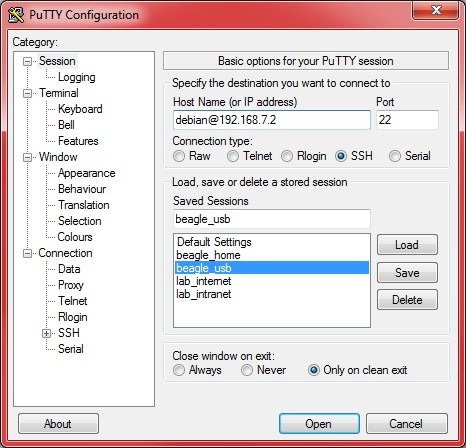
\includegraphics[scale=0.90]{./Resources/putty-cfg.jpg}
	\captionsetup{justification=centering}
	\caption[Configura��o do \textit{Putty} para acesso SSH via USB]{Configura��o do \textit{Putty} para acesso SSH via USB}
	\label{putty-cfg}
\end{figure}

\begin{figure}[H]
	\centering
	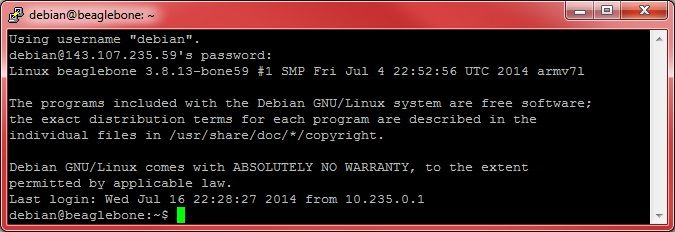
\includegraphics[scale=0.80]{./Resources/putty-first-login.jpg}
	\captionsetup{justification=centering}
	\caption[Tentativa de login bem sucedida pelo \textit{Putty}]{Tentativa de login bem sucedida pelo \textit{Putty}}
	\label{putty-flogin}
\end{figure}

\subsection{Ajustes de rede para uso do adaptador Wi-Fi/USB}

Para utilizar o adaptador Wi-Fi USB, em primeiro lugar este foi conectado � BBB. Em seguida, no terminal, o dispositivo foi listado para confirmar que o sistema estava identificando-o corretamente e ativado, permitindo assim obter a lista de redes Wi-Fi pr�ximas. Com isso, foi poss�vel obter os dados da rede Wi-Fi de interesse, para posterior edi��o do arquivo \textit{/etc/network/interfaces}, respons�vel pelas configura��es de rede do sistema -- este pode ser obtido no ap�ndice \ref{Ap�ndice B}. O c�digo \ref{wifi_conf} ilustra a sequ�ncia de comandos executados:

\lstset{language=bash}
\begin{lstlisting}[frame=single, basicstyle=\linespread{0.85}\ttfamily, caption=Passos para configura��o do Wi-Fi, label=wifi_conf]
lsusb # verifica se o dispositivo USB foi detectado
sudo ifconfig wlan up # ativa a interface de rede USB
sudo iwlist scan # lista as redes Wi-Fi dispon�veis

# Identificar os valores da rede de interesse, e.g.
#	ESSID:"Nome_da_rede" -> nome da rede
#	IE: IEEE 802.11i/WPA2 Version 1 -> encripta��o
# E ent�o � modificado o arquivo de configura��o

# abre o arquivo para edi��o
sudo nano /etc/network/interfaces 
# Ap�s modificar o arquivo e salv�-lo:

sudo ifup wlan0 # ativa a interface de rede Wi-Fi
sudo ifdown eth0 # desativa a interaface Ethernet

\end{lstlisting}

No arquivo \textit{/etc/network/interfaces}, as configura��es utilizadas entre as linhas 19 e 35 do c�digo s�o referentes � configura��o do Wi-Fi para configura��o da BBB com endere�o de IP est�tico 192.168.1.155, permitindo o acesso � plataforma remotamente pela internet e n�o somente dentro da intranet. Observe-se que o acesso a este IP da intranet se d� pelo IP externo 143.107.xxx.xxx, que � o endere�o do departamento da engenharia el�trica da USP de S�o Carlos. Por motivos de seguran�a este ser� omitido no presente trabalho.

Depois de todo este procedimento, o dispositivo ainda n�o estava funcionando ap�s a opera��o de \textit{reboot}, portanto foi utilizado um \textit{script} de reset do Wi-Fi executado durante o \textit{boot}, cujas instru��es de uso, obtidas em  \url{https://learn.adafruit.com/setting-up-wifi-with-beaglebone-black/configuration}, est�o descritas no c�digo-fonte \ref{rst_wifi}. A figura \ref{success_ssh} indica sucesso de conex�o via SSH usando uma m�quina com sistema operacional Linux Ubuntu 14.04 LTS.

\lstset{language=bash}
\begin{lstlisting}[frame=single, basicstyle=\linespread{0.85}\ttfamily, caption=Configura��o para reset do Wi-Fi ap�s o boot, label=rst_wifi]
git clone https://github.com/adafruit/wifi-reset.git #download do script
cd wifi-reset/ #entra no diret�rio do script
chmod +x install.sh #permiss�o de execu��o para o script
sudo ./install.sh #executa o script
\end{lstlisting}

\begin{figure}[H]
	\centering
	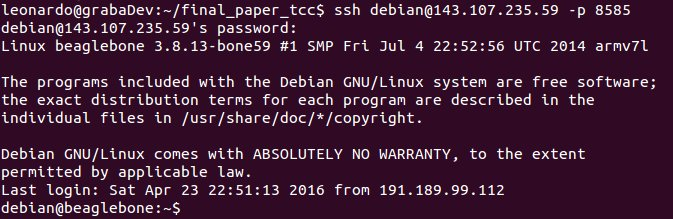
\includegraphics[scale=0.50]{./Resources/ssh_login_linux.jpg}
	\captionsetup{justification=centering}
	\caption[Acesso � BBB via SSH]{Acesso � BBB via SSH}
	\label{success_ssh}
\end{figure}

\subsection{Data/hora}

Para a configura��o autom�tica de data e hora da BBB, foi escolhido o uso do protocolo NTP -- \textit{Network Time Protocol} ou Protocolo de Tempo para Redes -- cujo objetivo � sincronizar os rel�gios de dispositivos conectados a uma rede a partir de fontes precisas \cite{ntp}. No Brasil, a confiabilidade deste protocolo � responsabilidade do Observat�rio Nacional (ON), respons�vel legal por garantir a Hora Legal Brasileira, em conjunto com o N�cleo de Informa��o e Coordena��o do Ponto BR, administrador e operador do dom�nio ".br"  \cite{nic,dsho}.

Primeiramente foi realizada a instala��o do protocolo, seguida da configura��o do arquivo \textit{/etc/ntp.conf} e da modifica��o do arquivo que indica a \textit{timezone}, sendo este um link simb�lico para o verdadeiro arquivo. Os comandos executados est�o descritos no c�digo-fonte \ref{ntp_install}:

\lstset{language=bash}
\begin{lstlisting}[frame=single, basicstyle=\linespread{0.85}\ttfamily, caption=Instala��o e configura��o do NTP, label=ntp_install]
sudo apt-get install ntp #instala o NTP
sudo nano /etc/ntp.conf #abre o arquivo de configura��o para edi��o
sudo mv /etc/localtime /etc/localtime-old #backup do arquivo antigo da timezone
sudo ln -s /usr/share/zoneinfo/America/Sao_Paulo /etc/localtime #cria link simb�lico para arquivo da nova timezone
\end{lstlisting}

Na edi��o do arquivo \textit{/etc/ntp.conf}, a �nica modifica��o feita � a substitui��o dos servidores de hora padr�o para os servidores brasileiros, listados no endere�o \url{http://www.pool.ntp.org/zone/br} -- no final de cada endere�o foi adicionada a instru��o \textit{iburst}, conforme descrito no website oficial do protocolo (\url{http://support.ntp.org/bin/view/Support/ConfiguringNTP}) e que, embora n�o esteja claro seu funcionamento, � essencial para que o hor�rio seja corretamente configurado a cada \textit{reboot}. O trecho de c�digo-fonte \ref{ntp_br} indica as modifica��es no arquivo \textit{/etc/ntp.conf} adequando aos servidores brasileiros:

\lstset{language=bash}
\begin{lstlisting}[frame=single, basicstyle=\linespread{0.85}\ttfamily, caption=Servidores brasileiros do NTP, label=ntp_br]
# You do need to talk to an NTP server or two (or three).
#server ntp.your-provider.example

# pool.ntp.org maps to about 1000 low-stratum NTP servers. Your server will
# pick a different set every time it starts up. Please consider joining the
# pool: <http://www.pool.ntp.org/join.html>
server 0.br.pool.ntp.org iburst
server 1.br.pool.ntp.org iburst
server 2.br.pool.ntp.org iburst
server 3.br.pool.ntp.org iburst
\end{lstlisting}

\subsection{Sensor DS18B20}

Uma vez que o sensor de temperatura DS18B20 j� � suportado pelo Kernel e inclu�do como \textit{driver} na distribui��o padr�o da BBB, somente foi necess�rio criar uma sobreposi��o de \textit{device tree} indicando em que pino o sensor est� ligado. Tanto o mux quanto o OCP do SoC precisaram ser configurados e, para a compila��o do arquivo texto em bin�rio, foi necess�ria a instala��o do DTC, descrita no c�digo-fonte \ref{dtc_install}:

\lstset{language=bash}
\begin{lstlisting}[frame=single, basicstyle=\linespread{0.85}\ttfamily, caption=Instala��o do DTC, label=dtc_install]
sudo wget -c https://raw.github.com/RobertCNelson/tools/master/pkgs/dtc.sh 
sudo chmod +x dtc.sh
./dtc.sh
\end{lstlisting}

O arquivo com a sobreposi��o da \textit{device tree} � descrito na se��o \ref{ap3ds18b20}, por�m o c�digo-fonte \ref{dtf_ds18b20} apresenta um trecho relevante deste, no qual observa-se a configura��o do multiplexador do SoC. Note-se que esta configura��o significa que o \textit{pull-up} interno de 10k\ohm da BBB est� ativado, eliminando a necessidade de um resistor externo. O valor m�nimo de \textit{pull-up} segundo a folha de dados do sensor � de 4,7k\ohm, mas n�o foi observada perda de desempenho do mesmo na presente configura��o.

\lstset{language=bash}
\begin{lstlisting}[frame=single, basicstyle=\linespread{0.85}\ttfamily, caption=Fragmento de device tree para o DS18B20, label=dtf_ds18b20]
bb_w1_pins: pinmux_bb_w1_pins {
	pinctrl-single,pins =  <0x70 0x37>;
};
\end{lstlisting}

A compila��o da sobreposi��o � executada com o comando presente no trecho de c�digo \ref{dtc_compile}. Adicionar "-00A0" ao nome do arquivo de sa�da DTBO � fundamental. Note-se tamb�m que o arquivo DTBO � copiado para o diret�rio no qual ficam todas as sobreposi��es de \textit{device tree}. Para carregar a sobreposi��o no boot, � preciso adicionar a linha \textit{echo w1 > /sys/devices/bone\_capemgr.*/slots} ao arquivo \textit{/etc/rc.local}.

\lstset{language=bash}
\begin{lstlisting}[frame=single, basicstyle=\linespread{0.85}\ttfamily, caption=Compila��o de \textit{device tree}, label=dtc_compile]
sudo dtc -O dtb -o w1-00A0.dtbo -b 0 -@ w1.dts
sudo cp w1-00A0.dtbo /lib/firmware
\end{lstlisting}

Ap�s o reboot e com o sensor conectado � BBB, � poss�vel obter o valor da temperatura realizando a leitura do arquivo \textit{/sys/devices/w1\_bus\_master1/28-*/w1\_slave}, conforme ilustrado na figura \ref{ds_reading}. Observe-se que na figura ao inv�s do asterisco foi utilizado o identificador �nico deste sensor espec�fico --- quando � utilizado um asterisco, ele � substitu�do por todos os poss�veis nomes de sensores, portanto � �til para leitura de diversos sensores de uma vez. Para saber quantos dispositivos com o protocolo \textit{1-wire} est�o conectados � mesma linha e assim descobrir os n�meros referentes a eles, � poss�vel ler o arquivo \textit{/sys/devices/w1\_bus\_master1/w1\_master\_slaves} ou ent�o verificar o conte�do do diret�rio \textit{/sys/devices/w1\_bus\_master1/}.

\begin{figure}[H]
	\centering
	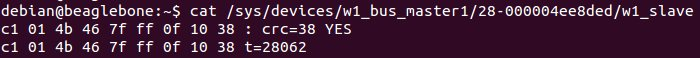
\includegraphics[scale=0.50]{./Resources/ds_reading_terminal.jpg}
	\captionsetup{justification=centering}
	\caption[Leitura do sensor DS18B20 pelo terminal]{Leitura do sensor DS18B20 pelo terminal}
	\label{ds_reading}
\end{figure}

\subsection{Webserver Apache}

Embora o Apache venha instalado na distribui��o padr�o da imagem do Debian para a BBB, � preciso configurar a porta que ele usa para conex�es, predefinida pelas configura��es de rede do departamento de engenharia el�trica. A porta ser� omitida por seguran�a, mas na descri��o do processo de configura��o aqui proposta ser� usado o valor 8080, padr�o para diversos protocolos de internet, inclusive o HTTP.

H� dois arquivos que devem ser editados para modificar as configura��es do Apache. No arquivo \textit{/etc/apache2/sites-enabled/000-default} a primeira linha do arquivo deve ser modificada para \textit{<VirtualHost *:8080>} e no arquivo \textit{/etc/apache2/ports.conf} as linhas \textit{NameVirtualHost *:8080} e \textit{Listen 8080} devem ser adicionadas ou modificadas, caso j� existam. Para que as configura��es tenham efeito, o servidor deve ser reiniciado com o comando descrito na caixa de c�digo-fonte \ref{restart_apache}:

\lstset{language=bash}
\begin{lstlisting}[frame=single, basicstyle=\linespread{0.85}\ttfamily, caption=Reinicializa��o do servidor web Apache, label=restart_apache]
sudo service apache2 restart
\end{lstlisting}


%%%%%%%%%%%%%%%%%%%%%%%%%%%%%%%%%%%%%%%%%%%%%%%%%%%%%%%%%%%%%%%%%%%%%%%%%%

\section{Organiza��o do diret�rio da aplica��o}
Dado o n�vel de complexidade a que chegou o desenvolvimento da aplica��o de controle do sistema, foi necess�rio adotar um sistema de divis�o de arquivos por fun��o. Dentre os tipos de arquivos h� principalmente c�digos-fonte, imagens e registros. O objetivo desta se��o � explicar a organiza��o adotada.

Cabe primeiramente observar que h� duas grandes frentes de projeto com rela��o a software: a aplica��o do servidor e a aplica��o do cliente. Uma vez que h� momentos em que ambas est�o entrela�adas, foi decidido por n�o separar os arquivos em pastas \textit{cliente} e \textit{servidor}, mas somente classificar cada arquivo como pertencente principalmente a uma destas duas frentes.

A tabela \ref{diretorios} lista os diret�rios e arquivos relevantes ao projeto, assim como uma breve descri��o destes e a distin��o dos arquivos entre \textit{cliente} ou \textit{servidor}.

\begin{center}
	\begin{table}[H]
		\centering
		\captionsetup{justification=centering}
		\caption[Estrutura de diret�rios e arquivos da aplica��o da BBB]{Estrutura de diret�rios e arquivos da aplica��o da BBB}
		\label{diretorios}
		\begin{tabular}{ | M{4cm} | M{9cm} | M{2cm} |}
			\hline
			\textbf{Diret�rio/arquivo} & \textbf{descri��o} & \textbf{Frente} \\ \hline
			
			\textbf{www} & \textbf{diret�rio raiz} & \\ \hline
			about.php & p�gina de descri��o do projeto & cliente \\ \hline
			control.php & GUI de controle do sistema & cliente \\ \hline
			controle.js & arquivo raiz da aplica��o do servidor & servidor \\ \hline
			dyn\_graph2.html & gr�fico din�mico de linha/�rea & cliente \\ \hline
			index.html & p�gina inicial - cont�m somente uma imagem clic�vel & cliente\\ \hline
			listrecipe.php & gerenciador de receitas - permite criar, editar e excluir & cliente\\ \hline
			newrecipe.php & GUI de edi��o de receitas & cliente \\ \hline
			settings.php & GUI de configura��es n�o referentes � brassagem & cliente \\ \hline
			startrecipe.php & escolha da receita e in�cio da brassagem & cliente \\ \hline
			stats.php & estat�sticas diversas de produ��es anteriores & cliente \\ \hline

			\textbf{www/css} & \textbf{configura��es de estilo da GUI} & \\ \hline
			buttons.css & estiliza alguns bot�es da GUI & cliente \\ \hline
			config.css & configura��es gerais de estilo da GUI & cliente \\ \hline
			form.css & estilo do formul�rio de edi��o de receitas & cliente \\ \hline

			\textbf{www/datalog} & \textbf{registros e backup de dados em mem�ria n�o vol�til} & \\ \hline
			backup.log & registro detalhado da �ltima brassagem & servidor \\ \hline
			default.csv & registro de temperaturas e tempos do DS18B20 & servidor \\ \hline
			instant.csv & �ltima leitura do DS18B20 da MT & servidor \\ \hline
			instant\_bk.csv & �ltima leitura do DS18B20 do BK & servidor \\ \hline
			lockfile & arquivo que define se h� uma brassagem em execu��o & servidor \\ \hline

			\textbf{www/img} & \textbf{imagens geradas para a GUI} & \\ \hline
			beer2.png & favicon & cliente \\ \hline
			beer\_compiler.png & imagem da p�gina inicial da GUI & cliente \\ \hline
			tplot.png & gr�fico est�tico da temperatura em fun��o do tempo & cliente \\ \hline

			\textbf{www/my\_node\_modules} & \textbf{m�dulos em Node.js desenvolvidos neste projeto} & \\ \hline
			ctrl.js & implementa��o do algoritmo de controle da brassagem & servidor \\ \hline
			gpio\_cfg.js & configura��o e controle de GPIO e PWM & servidor \\ \hline
			log\_check\_misc.js & verifica��o de integradade de receita. Leitura e registros de informa��es referentes � brassagem & servidor \\ \hline
			routes.js & rotas do servidor Express.js & servidor \\ \hline

			\textbf{www/lib} & \textbf{m�dulos requisitados por c�digos-fonte do cliente} & \\ \hline
			deleterecipe.php & deleta uma receita do servidor & servidor \\ \hline
			header.js & auxiliar de cria��o do cabe�alho da GUI & cliente \\ \hline
			header.php & cria��o do cabe�alho da GUI & cliente \\ \hline
			listrecipe.js & l� conte�do ou deleta receita do servidor & servidor \\ \hline
			newrecipe.js & organiza e salva automaticamente a GUI de edi��o de receitas & cliente / servidor \\ \hline
			newrecipe.php & salva ou carrega receita para a GUI de edi��o de receitas & servidor \\ \hline
			previewrecipe.php & l� conte�do essencial da receita e devolve para a GUI & cliente / servidor \\ \hline

			\textbf{log} & \textbf{registros de erros de aplica��es da BBB} & \\ \hline
			\textbf{recipes} & \textbf{receitas de cerveja} & \\ \hline
			\textbf{node\_modules} & \textbf{m�dulos do Node.js instalados por meio do NPM} & \\ \hline
			\textbf{d3-3.4.10} & \textbf{biblioteca Javascript de visualiza��o de dados} & \\ \hline
			\textbf{rickshaw} & \textbf{API de gera��o de gr�ficos baseada na biblioteca D3.js} & \\ \hline
			\textbf{tmp} & \textbf{diret�rio para testes e arquivos tempor�rios} & \\ \hline
		\end{tabular}
	\end{table}
\end{center}




%%%%%%%%%%%%%%%%%%%%%%%%%%%%%%%%%%%%%%%%%%%%%%%%%%%%%%%%%%%%%%%%%%%%%%%%%%

\section{IDE e sistema de controle de vers�o}
Para o desenvolvimento de software deste projeto, foram empregadas as ferramentas \textit{Cloud9} e GIT, que s�o uma IDE e um sistema de controle de vers�o, respectivamente. Informa��es sobre estas ferramentas e seu uso no projeto est�o contidas no ap�ndice \ref{git_apendice}.

%Para facilitar o desenvolvimento e a documenta��o de \textit{softwares}, duas ferramentas foram adotadas al�m do acesso ao sistema embarcado via SSH: \textit{Cloud9}, cujo uso � descrito na se��o \ref{c9} e \textit{Git/GitHub}, na se��o \ref{ghb}.

\section{\textit{Cloud9}}
\label{c9}

\textit{Cloud9} � um IDE do tipo \textit{software as a service} ou software como um servi�o (SaaS), ou seja, um software que est� na nuvem e cujo acesso � feito por meio de um navegador de internet. Embora o servi�o padr�o seja hospedado nos pr�prios servidores da \textit{Cloud9 IDE Inc.}, um SDK � disponibilizado, no qual est� incluso o n�cleo do projeto como c�digo-aberto, livre para uso n�o comercial e desenvolvido em Node.js. Isto possibilitou a hospedagem do servi�o do \textit{Cloud9} localmente na BBB\cite{c9_license}. Esta � uma n�tida vantagem para uma plataforma \textit{headless} --- sem perif�ricos do tipo \textit{human interface device} (HID) --- e com acesso � rede, a exemplo da BBB neste projeto, pois permite a programa��o direta no dispositivo por meio de uma interface gr�fica via web.

Tanto o n�cleo quanto as informa��es para instala��o podem ser encontradas no reposit�rio do projeto do \textit{GitHub} (\url{https://github.com/c9/core}). A primeira tentativa de instala��o realizado na BBB � apresentado na caixa de c�digo-fonte \ref{c9install}:

\lstset{language=bash}
\begin{lstlisting}[frame=single, basicstyle=\linespread{0.85}\ttfamily, caption=Primeira tentativa de instala��o do \textit{Cloud9 IDE core} na BBB, label=c9install]
cd ~/
git clone git://github.com/c9/core.git c9sdk
cd c9sdk
scripts/install-sdk.sh
\end{lstlisting}

Ao tentar executar a aplica��o apontando para o diret�rio \textit{/var/www} como diret�rio de projeto, ou seja, o diret�rio raiz ao qual o \textit{Cloud9} tem acesso, n�o foi poss�vel acessar os arquivos uma vez que o diret�rio em si pertencia ao usu�rio \textit{www-data} e os arquivos ao \textit{root}.

Ao rodar a aplica��o como administrador, outros erros ocorreram, o que levou � tentativa de instalar outro script presente no endere�o \url{https://github.com/c9/install} do reposit�rio do \textit{Cloud9}, que permite a conex�o da IDE a um servidor SSH. Ainda assim, os erros persistiram, o que levou � abertura de uma quest�o em \url{https://github.com/c9/core/issues/143}, na qual est� descrito o processo adotado para solucionar o problema. Na caixa de c�digo-fonte \ref{c9install_really} � apresentado o processo de instala��o executado com sucesso:

\lstset{language=bash}
\begin{lstlisting}[frame=single, basicstyle=\linespread{0.85}\ttfamily, caption=Instala��o bem sucedida do \textit{Cloud9 IDE core} na BBB, label=c9install_really]
cd ~/
wget --no-check-certificate https://raw.githubusercontent.com/c9/install/master/install.sh
sudo bash install.sh
\end{lstlisting}

Note-se que muitas tentativas foram executadas para obter o resultado final esperado, por isso em caso de tentativa de reprodu��o do processo de instala��o aqui descrito � recomendado tentar usar somente o processo da caixa de c�digo \ref{c9install_really} e, em caso de falha, partir para a etapa descrita anteriormente. Ainda assim, outro processo de instala��o mais direto e que deve ser tentado prioritariamente ao aqui descrito, mas que n�o foi testado, est� descrito em \url{https://cloud9-sdk.readme.io/docs/running-the-sdk}.

Para rodar a aplica��o no background e continuar executando mesmo ap�s desconectar da sess�o SSH, � preciso executar o servidor do \textit{Cloud9} como root usando o comando descrito na caixa \ref{c9start}. O par�metro \textit{-l} indica o endere�o de IP do servidor, \textit{-p} a porta, \textit{-a} usu�rio e senha e \textit{-w} o diret�rio de trabalho. Tamb�m s�o feitas redire��es das sa�das \textit{stdout} e \textit{stderr} para os arquivos \textit{/var/www/log/cl9.out} e \textit{/var/www/log/cl9.err}, respectivamente.

\lstset{language=bash}
\begin{lstlisting}[frame=single, basicstyle=\linespread{0.85}\ttfamily, caption=Execu��o do \textit{Cloud9}, label=c9start]
sudo su #precisa ser root
cd /home/debian #pasta na qual esta instalado o Cloud9
nohup node c9sdk/server.js -l 143.107.xxx.xxx -p xxxx -a usuario:senha -w /var/www/ > /var/www/log/cl9.out 2> /var/www/log/cl9.err < /dev/null &
\end{lstlisting}

Ao realizar o acesso pelo navegador usando o IP e porta selecionados, ou seja, digitando \textit{IP:porta} na URL do navegador, o resultado � apresentado na figura \ref{c9ide}. Note-se que o ambiente apresentado � a configura��o de IDE completa, mas que � completamente personaliz�vel, al�m de existirem outros \textit{presets}, dentre os quais um modo minimalista no qual somente o editor de texto ocupa a tela, bom para momentos de desenolvimento intensivo de um arquivo espec�fico.

\begin{figure}[H]
	\centering
	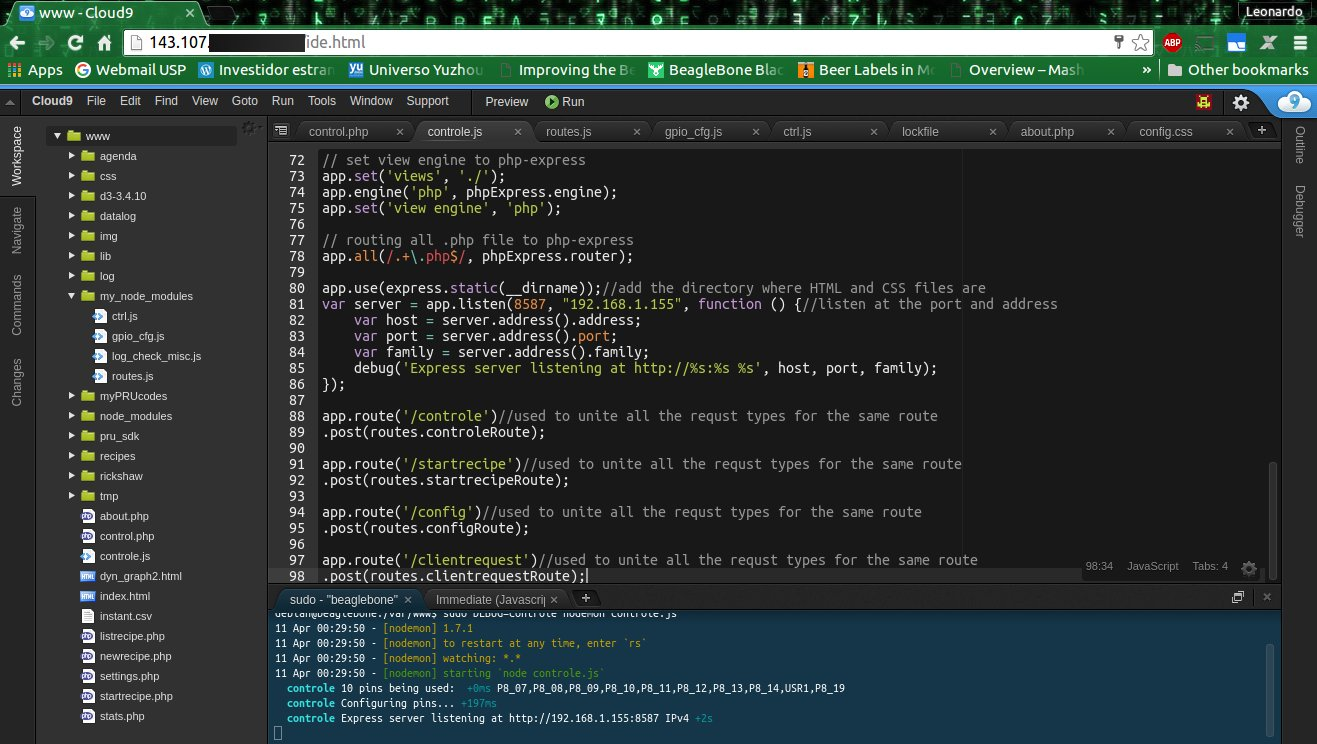
\includegraphics[scale=0.25]{./Resources/cloud9.jpg}
	\captionsetup{justification=centering}
	\caption[Ambiente completo do IDE \textit{Cloud9}]{Ambiente completo do IDE \textit{Cloud9}}
	\label{c9ide}
\end{figure}

\section{\textit{Git/GitHub}}
\label{ghb}

\textit{Git} � um sistema de controle de vers�o distribu�do (DVCS) e tamb�m � referido como um SCM (gerenciador de c�digos-fonte), ou seja, uma ferramenta cuja finalidade � gerenciar o desenvolvimento de \textit{software}. Um dos principais objetivos de um sistema como este � a documenta��o das mudan�as feitas nos arquivos do projeto ao longo do seu desenvolvimento, o que permite facilmente reverter arquivos ou mesmo o projeto inteiro para um estado anterior, comparar mudan�as em fun��o do tempo, verificar quem foi a �ltima pessoa a modificar um arquivo e possivelmente introduzir um bug, dentre outros recursos. E o mais importante, executar todas estas fun��es de maneira leve no que diz respeito a recursos computacionais e f�cil do ponto de vista do usu�rio \cite{git_book}.

Esta ferramenta foi escolhida dentre muitas outras DVCS dispon�veis por ser de c�digo-aberto e extremamente popular, n�o somente pelas suas qualidades mas tamb�m pelo fato de ser a DCVS usada para o controle de vers�o do Kernel do Linux, sendo que o \textit{Git} foi criado pela pr�pria comunidade de manuten��o do Kernel, incluindo Linus Torvalds \cite{git_book}. Embora a refer�ncia bibliogr�fica consultada sobre este assunto possua mais de 500 p�ginas, demonstrando o n�vel de complexidade que a ferramenta pode atingir, neste projeto somente o essencial ser� abordado --- o que significa compreender o uso de alguns comandos b�sicos.

Com rela��o ao \textit{GitHub}, este nada mais � do que um servi�o de hospedagem de reposit�rios \textit{Git}. Uma de suas grandes vantagens � a popularidade, o que o faz ser uma fonte repleta de recursos de c�digo-aberto. No que diz respeito a este trabalho, dentre suas vantagens est�o o fato de o servi�o facilitar o processo de \textit{backup} de todo o desenvolvimento realizado no �mbito de \textit{software}, prover uma estrutura que permite a replica��o do projeto com poucos comandos e tamb�m o uso deste servi�o para a reda��o da presente monografia sem a preocupa��o de ter que levar os arquivos fisicamente a diversas localidades ou depender de servi�os de armazenamento de prop�sito geral, que n�o apresentam as vantagens de um DVCS.

Para configurar uma conta no \textit{Github}, o primeiro passo foi a realiza��o do cadastro em \url{https://github.com}, seguida da cria��o de um reposit�rio online, conforme ilustrado na figura \ref{gitcreate}. Ap�s isto, o reposit�rio foi clonado na BBB e os arquivos relevantes do sistema foram copiados para ele. Observe-se que esta abordagem foi improvisada devido ao fato de arquivos de configura��o, dentre outros, encontrarem-se em reposit�rios espec�ficos do sistema, j� que o mais adequado seria que todos os arquivos do projeto fossem criados na pasta do \textit{Git}. Para instalar, configurar o \textit{Git} e clonar o reposit�rio rec�m criado do \textit{GitHub} para a BBB, foram executados os comandos descritos na caixa de c�digo-fonte \ref{install_git}.

\begin{figure}[H]
	\centering
	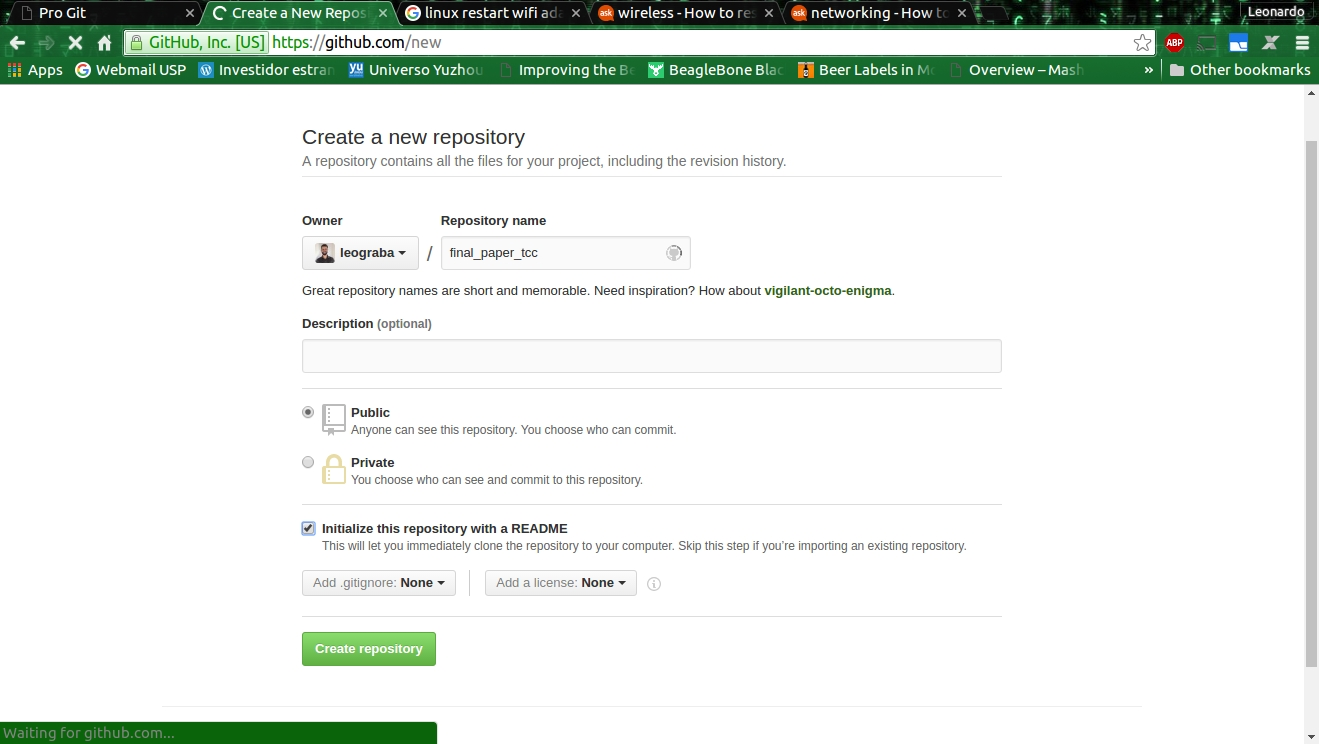
\includegraphics[scale=0.30]{./Resources/git-repo-creation.jpg}
	\captionsetup{justification=centering}
	\caption[Cria��o de reposit�rio no \textit{GitHub}]{Cria��o de reposit�rio no \textit{GitHub}}
	\label{gitcreate}
\end{figure}

\lstset{language=bash}
\begin{lstlisting}[frame=single, basicstyle=\linespread{0.85}\ttfamily, caption=Instala��o do \textit{Git} e c�pia do reposit�rio do \textit{GitHub} para a BBB, label=install_git]
sudo apt-get install git
git configure --global user.name "Nome"
git configure --global user.email email@exemplo.com
cd ~
git clone https://github.com/leograba/final_paper_tcc.git
\end{lstlisting}

Ap�s a clonagem do diret�rio \textit{final\_paper\_tcc} do \textit{GitHub} para a BBB, todos os arquivos relevantes ao projeto foram copiados para ele e, subsequentemente, adicionados ao \textit{Git}: sempre que um arquivo � adicionado ou modificado em um reposit�rio \textit{Git}, ele � ignorado a menos que seja executado o comando \textit{git add arquivo} --- isto permite flexibilidade, principalmente com rela��o a arquivos que n�o devem ser adicionados ao reposit�rio, como arquivos auxiliares gerados por compiladores, por exemplo. Ap�s cada mudan�a, para torn�-la efetiva � preciso executar o comando \textit{git commit -m "mensagem para registro"}, que al�m da data e hora da modifica��o, permite adicionar uma mensagem para identificar o que foi modificado desde o �ltimo \textit{commit}. Por fim, foi preciso enviar as mudan�as do reposit�rio local para o \textit{GitHub}. O processo de adicionar arquivos novos/modificados, fazer \textit{commit} nas mudan�as e atualizar a origem remota est� descrito no c�digo-fonte \ref{git_commit} e foi usado sempre que mudan�as foram feitas ao projeto, desde implementa��es de funcionalidades a corre��es de \textit{bugs}. Um exemplo de \textit{commit} ap�s mudan�as incrementais � apresentado na figura \ref{commit_terminal}.

\lstset{language=bash}
\begin{lstlisting}[frame=single, basicstyle=\linespread{0.85}\ttfamily, caption=Primeiro \textit{git commit}, label=git_commit]
git add .
git commit "Primeiro commit"
git push origin master
\end{lstlisting}

\begin{figure}[H]
	\centering
	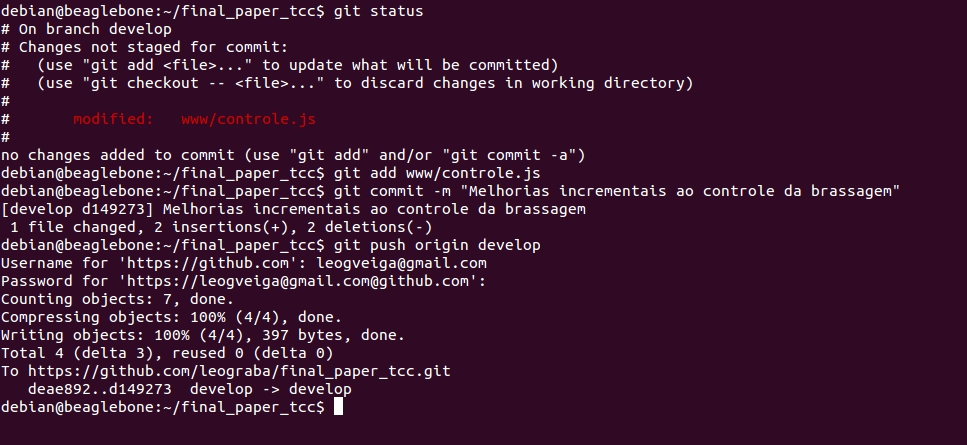
\includegraphics[scale=0.40]{./Resources/git-edit.jpg}
	\captionsetup{justification=centering}
	\caption[Fazendo \texit{git commit} ap�s mudan�as incrementais]{Fazendo \texit{git commit} ap�s mudan�as incrementais}
	\label{commit_terminal}
\end{figure}


%%%%%%%%%%%%%%%%%%%%%%%%%%%%%%%%%%%%%%%%%%%%%%%%%%%%%%%%%%%%%%%%%%%%%%%%%%

\section{Gera��o de gr�fico e registro de temperatura em Python}
Para o armazenamento da temperatura do sensor em fun��o do tempo, assim como a gera��o de um gr�fico com o hist�rico de temperaturas para o usu�rio do sistema, foram escritos dois \textit{scripts} em Python, sendo a sa�da do \textit{script} de \textit{log} a entrada do \textit{script} de gera��o do gr�fico --- embora ambos possam ser executados independentemente, a gera��o do gr�fico precisa de um arquivo contendo o hist�rico de temperaturas.

\subsection{Registro de temperatura}
\label{python_sec}
Para o arquivo do \textit{log}, foram primeiramente escritas algumas fun��es:

\begin{itemize}
	\item \textbf{tread()} --- l� o arquivo referente ao sensor de temperatura e retorna deste somente a temperatura formatada em graus celsius.
	\item \textbf{tprint\_all(tcelsius)} ---  recebe temperatura em \si{\degree}C e imprime com formata��o HTML em \si{\degree}C, \si{\degree}F, K e \si{\degree}R; pode ser usada em conjunto com a fun��o tread()
	\item \textbf{tprint\_all\_terminal(tcelsius)} ---  id�ntica � fun��o tprint\_all(), por�m imprime com formata��o
para o terminal do Linux
	\item \textbf{tlog(file = "/var/www/default.csv")} --- cria/adiciona a um arquivo de log no formato CSV a
temperatura medida e a data/hora correspondente no formato \textit{Unix epoch} --- que � definido como o n�mero de segundos passados desde 1 de janeiro de 1970 n�o considerando segundos bissextos --- em intervalo de amostragem definido na fun��o, at� que o script seja interrompido de alguma maneira. Em fun��o de erros de leitura espor�dicos do sensor, se a temperatura lida for menor ou igual a zero, esta � descartada. Imprime a temperatura lida a cada amostragem. O tempo de amostragem � definido pela soma do tempo de leitura do arquivo (inerente ao sistema) com o tempo ocioso definido nesta fun��o: para que o tempo de amostragem seja o mais pr�ximo poss�vel de 1s, foi realizado um estudo de caso, descrito no ap�ndice \ref{analise_tread_temp}, e com isso obteve-se o valor de 0,2202s ocioso definido nesta fun��o. Al�m disto, nesta fun��o � chamada \textit{tlog\_instant} que registra em um arquivo separado a �ltima leitura v�lida de temperatura e tempo.
	\item \textbf{tlog\_instant(temperature, epoch, file = "/var/www/datalog/instant.csv")} --- registra a �ltima leitura v�lida de temperatura e tempo em um arquivo, criando ou sobrescrevendo o mesmo.
	\item \textbf{tlog\_test(file = "/var/www/datalog/default.csv")} --- fun��o que gera um arquivo de \textit{log} com rampas e degraus de temperatura, para uso em simula��es posteriores do funcionamento do sistema, descritas na se��o \ref{simulacao_controle}.
\end{itemize}

Sendo a fun��o \textit{tlog} a mais relevante, esta pode ser obtida na caixa de c�digo-fonte \ref{tlog_python}. O script completo est� registrado no c�digo-fonte \ref{python_log_script} do ap�ndice \ref{codigos_python}. Ainda assim, as fun��es por si s� n�o s�o executadas sozinhas, portanto foi criado um script auxiliar em Python que chama a fun��o \textit{tlog}, descrito no c�digo-fonte \ref{tlog_log}.

\lstset{language=Python}
\begin{lstlisting}[frame=single, basicstyle=\linespread{0.85}\ttfamily, caption=Fun��o de \textit{log} da temperatura em Python, label=tlog_python]
def tlog(file = "/var/www/datalog/default.csv"):
	"""salva temperatura e Unix Time em .csv """
	tsample = 0.2202 #amostra a cada ~1 segundo
	buff_temp = tread()#guarda o �ltimo valor lido
	exist = os.path.isfile(file)
	with open(file, 'a', 1) as log:
		if exist is False:#se vai criar o arquivo agora
			log.write("temperatura,data\n")
		while True: #loop infinito
			temp_celsius = tread()
			epoch = time.time()#l� a data/hora do sistema
			if temp_celsius >= 0:#evita leitura errada
				log.write("%f,%f\n" % (temp_celsius, epoch))
				tlog_instant(temp_celsius, epoch)
				time.sleep(tsample)#espera n segundos
				print "registrando temperatura!",temp_celsius
\end{lstlisting}

\lstset{language=Python}
\begin{lstlisting}[frame=single, basicstyle=\linespread{0.85}\ttfamily, caption=Script para grava��o das leituras de temperatura em Python, label=tlog_log]
import temp
temp.tlog()
# para executar no terminal, basta executar:
# sudo python log.py
\end{lstlisting}

Na figura \ref{csv_log_example} � apresentada uma amostra de arquivo CSV gerado pelo script \ref{tlog_log}, e que valida o funcionamento da aplica��o.

\begin{figure}[H]
	\centering
	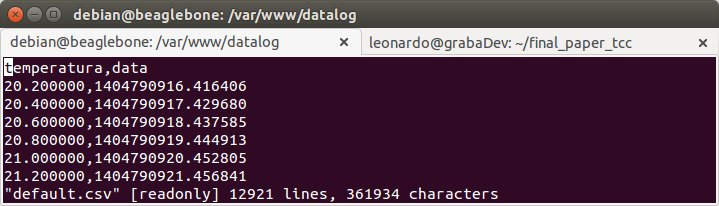
\includegraphics[scale=0.50]{./Resources/csv_log_example.jpg}
	\captionsetup{justification=centering}
	\caption[Arquivo CSV com registro de temperaturas gerado em Python]{Arquivo CSV com registro de temperaturas gerado em Python}
	\label{csv_log_example}
\end{figure}

\subsection{Gr�fico de temperatura}
\label{python_graph}

Com o script que gera um registro da temperatura medida pelo sensor DS18B20 em fun��o do tempo, o pr�ximo passo � a an�lise dos dados coletados. Uma forma faz�-lo � plotando um gr�fico. Para faz�-lo em Python, foi decido usar as bibliotecas \textit{Matplotlib} e \textit{NumPy}, integrantes do ecossistema \textit{SciPy}.

\textit{Matplotlib} � uma biblioteca desenvolvida especificamente para a plotagem 2D de figuras est�ticas em scripts Python, no Python shell (similar ao ambiente interpretador de \textit{softwares} propriet�rios como MATLAB e Mathematica), em aplica��es de servidores e \textit{toolkits} com GUI \cite{matplotlib}. Para instalar esta biblioteca, basta executar o comando descrito na caixa de c�digo-fonte \ref{install_matplotlib}.

\lstset{language=bash}
\begin{lstlisting}[frame=single, basicstyle=\linespread{0.85}\ttfamily, caption=Instala��o da biblioteca Matplotlib, label=install_matplotlib]
sudo apt-get install python-matplotlib
\end{lstlisting}

\textit{NumPy} � um pacote em Python que fornece suporte a arranjos e matrizes multidimensionais, al�m de diversas fun��es matem�ticas de suporte a estes formatos de dados. � amplamente empregado nas �reas de computa��o cient�fica, engenharia e matem�tica \cite{numpy}. Este pacote � parte integrante do ecossistema \textit{SciPy}, cuja instala��o � apresentada na caixa de c�digo-fonte \ref{install_scipy}.

\lstset{language=bash}
\begin{lstlisting}[frame=single, basicstyle=\linespread{0.85}\ttfamily, caption=Instala��o do ecossistema SciPy, label=install_scipy]
sudo apt-get install python-scipy
\end{lstlisting}

\subsubsection{Desenvolvimento do gr�fico}

Com todas as ferramentas necess�rias instaladas, p�de ser iniciado o desenvolvimento do script que gera o gr�fico da temperatura em fun��o do tempo. A abordagem inicial foi criar um script que gera um arquivo PDF do gr�fico a partir do exemplo encontrado na p�gina \url{http://matplotlib.org/examples/pylab_examples/multipage_pdf.html} , modificando este script para as necessidades do projeto.

Como o desenvolvimento foi realizado sem uma interface gr�fica, referida como \textit{backend}, foi preciso explicitar a sa�da como um renderizador no lugar deste, conforme indicado no c�digo-fonte \ref{import_py}, que documenta a importa��o das bibliotecas/fun��es utilizadas no script. Note-se que a mudan�a da sa�da deve ocorrer antes da importa��o da biblioteca \textit{numpy} para que n�o ocorra erro.

\lstset{language=Python}
\begin{lstlisting}[frame=single, basicstyle=\linespread{0.85}\ttfamily, caption=Importa��o das bibliotecas para gera��o de gr�fico em Python, label=import_py]
import time
import matplotlib
matplotlib.use('AGG')#muda a output para um renderer ao inves de backend
import numpy as np
import matplotlib.pyplot as plt
from scipy import interpolate
\end{lstlisting}

Na �nica fun��o do script, \textit{graph\_gen(file = '/var/www/default.csv', graph = '/var/www/tplot.png')}, � explicitado que a entrada � um arquivo CSV e a sa�da um arquivo PNG. Nesta fun��o o arquivo CSV � lido linha por linha em um \textit{loop}, sendo a primeira linha do arquivo ignorada em fun��o de ela n�o conter dados, conforme ilustrado na figura \ref{csv_log_example}. Ao longo das itera��es deste \textit{loop}, a data/hora do primeiro e �ltimo registro de temperatura s�o usadas para gerar um t�tulo para o gr�fico e, a cada itera��o os dados s�o decodificados, o que se resume basicamente a separar o que h� antes e depois da v�rgula presente na linha lida do arquivo CSV.

Na parte da fun��o referente � plotagem do gr�fico, al�m de configura��es triviais como cor de fundo, tamanho de fontes e legendas, dentre outros, � not�vel o ajuste da escala do tempo, para o qual foi pensado um registro de temperatura cont�nuo e n�o somente o registro de uma produ��o de cerveja: para at� duas horas de registro a escala � impressa em minutos; entre duas horas e um dia e meio de registros, em horas; entre um dia e meio e tr�s meses de registros, em dias; e acima disto em meses. Ap�s isto, o gr�fico � plotado, salvo no formato PNG com densidade de pontos por polegada de 150dpi, e fechado para liberar a mem�ria do sistema.

O script que chama a fun��o \textit{graph\_gen} � descrito no c�digo-fonte \ref{gen_graph}, presente no mesmo arquivo em que est� a fun��o. Note-se que o gr�fico � gerado periodicamente a cada 300 segundos e o tempo necess�rio para executar tal tarefa � computado e impresso na sa�da padr�o do Python. O arquivo completo que cont�m a fun��o \textit{graph\_gen} est� documentado no c�digo-fonte \ref{python_graph_script} do ap�ndice \ref{codigos_python}.

Na figura \ref{py_graph_7200p} � apresentado um gr�fico gerado na BBB a partir de 7200 pontos amostrados, ou seja, 120 minutos. Este tempo foi escolhido uma vez que dificilmente o cozimento do mosto ou a fervura dura mais do que isso, portanto provando que a implementa��o � fact�vel para o uso a que se destina. A tabela  \ref{tabela_tempo_graph_python} apresenta informa��es estat�sticas sobre o tempo de computa��o necess�rio para a gera��o do gr�fico. A figura \ref{amostras_graph} apresenta o processo de verifica��o do n�mero de pontos registrados e o posterior processo de coleta dos dados que deram origem � tabela \ref{tabela_tempo_graph_python}.

\begin{figure}[H]
	\centering
	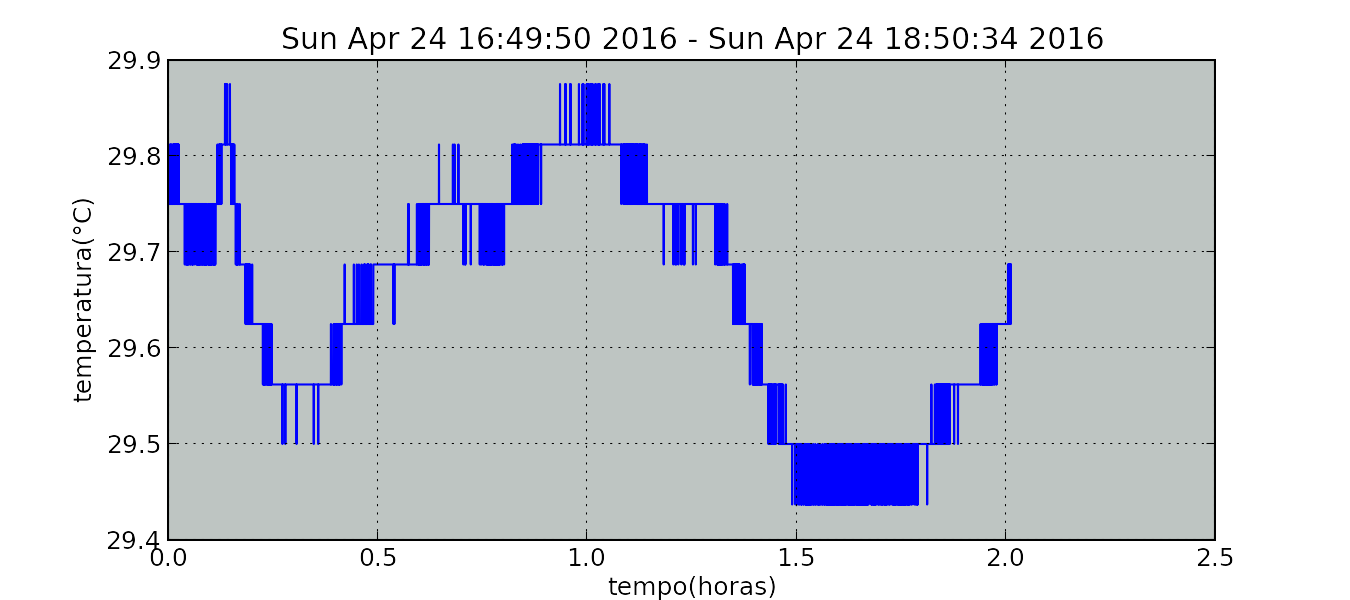
\includegraphics[scale=0.65]{./Resources/py_graph_7200p.png}
	\captionsetup{justification=centering}
	\caption[Gr�fico com 7200 pontos gerado em Python]{Gr�fico com 7200 pontos gerado em Python}
	\label{py_graph_7200p}
\end{figure}

%\begin{center}
	\begin{table}[H]
		\centering
		\captionsetup{justification=centering}
		\caption[Estat�sticas referentes ao tempo de gera��o de gr�fico na BBB, para 7200 pontos em Python]{Estat�sticas referentes ao tempo de gera��o de gr�fico na BBB, para 7200 pontos em Python}
		\label{tabela_tempo_graph_python}
		\begin{tabular}{ | M{5cm} | M{2cm} |}
			\hline
			\textbf{Descri��o} & \textbf{Valor} \\ \hline
			N.\si{\degree} de amostras & 30\\ \hline
			M�dia (s) & 2,106\\ \hline
			M�ximo (s) & 2,068\\ \hline
			M�nimo (s) & 2,149\\ \hline
			Desvio padr�o (s) & 0,023\\ \hline
		\end{tabular}
	\end{table}
%\end{center}

\begin{figure}[H]
	\centering
	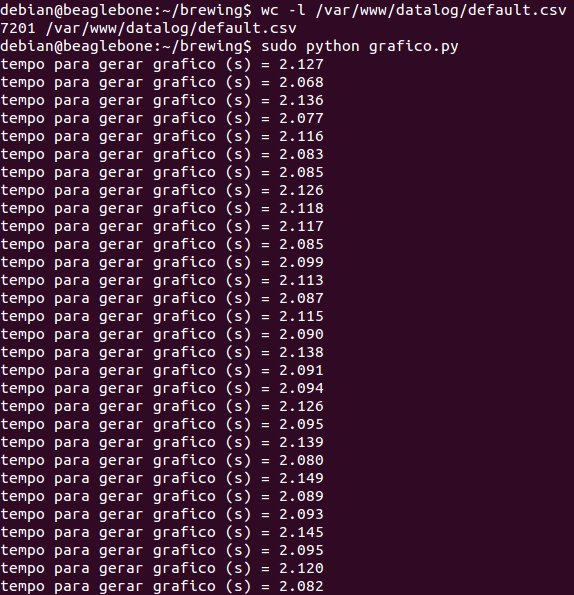
\includegraphics[scale=0.50]{./Resources/log_py_graph_7200p.jpg}
	\captionsetup{justification=centering}
	\caption[Gera��o de gr�fico em Python m�ltiplas vezes para obter o tempo m�dio]{Gera��o de gr�fico em Python m�ltiplas vezes para obter o tempo m�dio}
	\label{amostras_graph}
\end{figure}


%%%%%%%%%%%%%%%%%%%%%%%%%%%%%%%%%%%%%%%%%%%%%%%%%%%%%%%%%%%%%%%%%%%%%%%%%%

\section{Aplica��o \textit{server-side} em Node.js}
\label{nodectrl_sec}
Nesta se��o ser� detalhado o uso da linguagem de programa��o Javascript no ambiente de interpreta��o Node.js. O escopo da aplica��o desta linguagem no projeto se aplica, mas n�o � limitado a: acesso ao \textit{hardware}, incluindo barramentos de prop�sito geral (GPIO) e perif�ricos como PWM; cria��o de um servidor web minimalista; e controle do processo de produ��o de cerveja. Node.js j� vem instalado na distribui��o padr�o do Debian utilizada neste projeto, por�m � poss�vel instalar ou atualizar o ambiente por meio do gerenciador de pacotes \textit{apt-get}, conforme descrito na caixa de c�digo-fonte \ref{install_node}:

\lstset{language=bash}
\begin{lstlisting}[frame=single, basicstyle=\linespread{0.85}\ttfamily, caption=Instala��o e/ou atualiza��o do Node.js, label=install_node]
sudo apt-get install nodejs
\end{lstlisting}

Com isto, o gerenciador de pacotes do Node chamado NPM (Node Package Manager) tamb�m � instalado no sistema. Neste projeto, o desenvolvimento em Node foi legado do desenvolvimento pr�vio em PHP e, por isto, tudo foi realizado no diret�rio \textit{/var/www}, cujo dono � o usu�rio \textit{www-data}. Em fun��o disto, foi criada manualmente a pasta \textit{/var/www/node\_modules} e o dono foi trocado para o usu�rio \textit{debian} (enquanto sob condi��es normais este processo seria autom�tico). Para evitar este problema, os m�dulos poderiam ser instalados globalmente, por�m por quest�es de seguran�a, esta foi a abordagem realizada, uma vez que os m�dulos do Node ficam autocontidos no diret�rio do projeto. O processo de cria��o do diret�rio \textit{/var/www/node\_modules} � descrito no trecho de c�digo \ref{create_node_modules}:

\lstset{language=bash}
\begin{lstlisting}[frame=single, basicstyle=\linespread{0.85}\ttfamily, caption=Cria��o do diret�rio \textit{/var/www/node\_modules}, label=create_node_modules]
cd /var/www
sudo mkdir node_modules
sudo chown debian:debian node_modules
\end{lstlisting}

Al�m disto, foi instalado o m�dulo \textit{Debug} do Node, que ajuda no desenvolvimento da aplica��o da seguinte maneira: ele encapsula a fun��o nativa do Javascript \textit{console.log}, an�loga ao \textit{printf} da linguagem C, de tal maneira que as mensagens s� s�o impressas na tela se a vari�vel \textit{DEBUG} estiver configurada no terminal durante a execu��o da aplica��o. Al�m disto, diferentes grupos de mensagens de \textit{debug} podem ser configurados, permitindo flexibilidade. Para diferenciar estes grupos, o m�dulo adota um esquema de cores que facilita a compreens�o das mensagens de \textit{debug}. 

Para ilustrar seu uso, na caixa \ref{install_debug} � descrita a instala��o do m�dulo; o trecho de c�digo-fonte \ref{debug_example} descreve como usar o m�dulo em uma aplica��o de Node e a figura \ref{debug_complex} apresenta o resultado do exemplo, para as seguintes situa��es: n�o imprime mensagens de debug; imprime grupos de mensagens de debug e; imprime todas as mensagens de debug dispon�veis.

\lstset{language=bash}
\begin{lstlisting}[frame=single, basicstyle=\linespread{0.85}\ttfamily, caption=Instala��o do m�dulo \textit{Debug}, label=install_debug]
npm install debug
\end{lstlisting}

\lstset{language=javascript}
\begin{lstlisting}[frame=single, basicstyle=\linespread{0.85}\ttfamily, caption=Exemplo de uso do m�dulo \textit{Debug}, label=debug_example]
"use strict";

var dbg_gpio = require('debug')('gpio');
var dbg_pwm = require('debug')('pwm');

console.log("Inicio exemplo:");
for(var i = 0; i < 3; i++){
	switch(i){
	case 0:
		dbg_gpio("Debug situacao gpio");
		break;
	case 1:
		dbg_pwm("Debug situacao pwm");
		break;
	case 2:
		dbg_gpio("Debug ambos gpio");
		dbg_pwm("Debug ambos pwm");
		break;
	}
}
\end{lstlisting}

\begin{figure}[H]
	\centering
	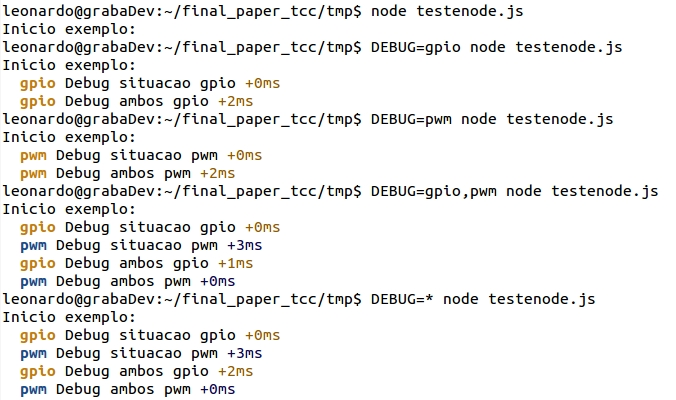
\includegraphics[scale=0.65]{./Resources/debug.jpg}
	\captionsetup{justification=centering}
	\caption[Exemplo de uso do m�dulo \textit{Debug}]{Exemplo de uso do m�dulo \textit{Debug}}
	\label{debug_complex}
\end{figure}

Neste cap�tulo deve-se assumir que todas as opera��es realizadas e arquivos referidos est�o no diret�rio \textit{/var/www}, salvo indica��es em contr�rio. Note-se tamb�m que, no in�cio dos c�digos-fonte completos, presentes no ap�ndice \ref{codigos_nodejs}, � usada a delcara��o \textbf{"use-strict"}, que evita o uso de potenciais armadilhas do Javascript, e.g. usar inadvertidamente uma vari�vel global sem delcar�-la.

\subsection{Acesso a GPIO e PWM}
\label{gpio_sec}

O acesso �s caracter�sticas de \textit{hardware} da BBB necess�rias para o controle das v�lvulas, bombas, resistores de pot�ncia e servo-motor do sistema � feito por meio do m�dulo de c�digo-aberto \textit{Octalbonescript}, que consiste de um \textit{fork} (ou deriva��o) do m�dulo oficial da BBB de acesso a hardware, chamado \textit{Bonescript}. Sua escolha se deve ao fato de que esta biblioteca era mais completa e est�vel durante o desenvolvimento deste projeto do que aquela que lhe deu origem. Sua instala��o est� descrita na caixa \ref{install_octalbonescript}. A documenta��o da API deste m�dulo foi obtida em \url{https://github.com/theoctal/octalbonescript/wiki}.

\lstset{language=bash}
\begin{lstlisting}[frame=single, basicstyle=\linespread{0.85}\ttfamily, caption=Instala��o do Octalbonescript, label=install_octalbonescript]
npm install octalbonescript
\end{lstlisting}

Uma vez que este m�dulo compila uma sobreposi��o de \textit{device tree} a partir de um template fornecido junto com a instala��o, foi necess�rio modific�-lo para acomodar a descri��o de hardware do sensor DS18B20. Para tal, foi investigado que o comportamento da biblioteca \textit{Octalbonescript} com rela��o � \textit{device tree} � o seguinte: se a sobreposi��o j� est� carregada n�o � feita nova compila��o do fragmento nem tentativa de carreg�-la novamente, portanto foi necess�rio resetar a BBB toda vez que novos testes eram realizados.

O template editado fica no diret�rio \textit{node\_modules/octalbonescript/dts/} e o nome do arquivo modificado � \textit{OBS\_UNIV\_template.dts}. As modifica��es realizadas, assim como as linhas do c�digo modificadas est�o descritas na caixa de c�digo-fonte \ref{octal_dts}. Linhas que come�am com "X" foram apagadas, as outras foram adicionadas.

\lstset{language=dtc}
\begin{lstlisting}[frame=single, basicstyle=\linespread{0.85}\ttfamily, caption=Modifica��es feitas ao template de \textit{device tree} do Octalbonescript, label=octal_dts]
[389]        /* P9_11 (THE ONE-WIRE DS18B20) */
[390]        bb_w1_pins: pinmux_bb_w1_pins {
[391]           pinctrl-single,pins = <0x070  0x37>; };     /* Mode 7, Pull-Up, RxActive */
X[392]        P9_11_gpio_pin: pinmux_P9_11_gpio_pin {
X[393]           pinctrl-single,pins = <0x070  0x2F>; };     /* Mode 7, RxActive */
X[394]        P9_11_gpio_pu_pin: pinmux_P9_11_gpio_pu_pin {
X[395]           pinctrl-single,pins = <0x070  0x37>; };     /* Mode 7, Pull-Up, RxActive */
X[396]        P9_11_gpio_pd_pin: pinmux_P9_11_gpio_pd_pin {
X[397]           pinctrl-single,pins = <0x070  0x27>; };     /* Mode 7, Pull-Down, RxActive */
X[398]        P9_11_uart_pin: pinmux_P9_11_uart_pin {
X[399]           pinctrl-single,pins = <0x070  0x36>; };     /* Mode 6, Pull-Up, RxActive */
[879]        onewire@0 {
[880]           compatible = "w1-gpio";
[881]           status = "okay";
[882]           pinctrl-names = "default";
[883]           pinctrl-0 = <&bb_w1_pins>;
X[884]           pinctrl-1 = <&P9_11_gpio_pin>;   gpios = <&gpio1 30 0>;
X[885]           pinctrl-2 = <&P9_11_gpio_pu_pin>;
X[886]           pinctrl-3 = <&P9_11_gpio_pd_pin>;
X[887]           pinctrl-4 = <&P9_11_uart_pin>;
[888]        };
X[1232]        P9_11 {
X[1233]           gpio-name = "P9_11";
X[1234]           gpio = <&gpio1 30 0>;
X[1235]           input;
X[1236]           dir-changeable;
X[1237]        };
\end{lstlisting}

Com esta configura��o da \textit{device tree}, foi preciso parar de carregar o fragmento descrito na se��o \ref{ds18b20_dev_tree}, pois ao tentar usar o \textit{Octalbonescript}, passou a ocorrer um erro do tipo \textbf{EEXIST: file already exists}, que indica em um �mbito geral que um arquivo que deveria ser criado j� existe.

A partir deste ponto, foi desenvolvido um m�dulo em Node nomeado \textit{gpio\_config} respons�vel pelo gerenciamento de GPIO e PWM, baseado no \texit{Octalbonescript}. Foram criados objetos para cada elemento do sistema, usados para guardar a identifica��o do pino de GPIO de cada objeto, o estado e a configura��o de cada pino. Para isto, uma fun��o auxiliar foi criada.

Tamb�m foi criado um objeto que re�ne todos os objetos dos pinos, para facilitar a configura��o inicial e tamb�m manter controle sobre o status do sistema durante seu funcionamento. Uma vez que em Node os objetos s�o todos ponteiros, ao atribuir um objeto a outro, o que se est� fazendo � apontar os dois objetos para o mesmo endere�o de mem�ria. A descri��o completa das declara��es de objetos pode ser encontrada no c�digo-fonte \ref{gpio_cfg} no ap�ndice \ref{codigos_nodejs}.

%Na caixa de c�digo-fonte \ref{gpio_variables} � apresentada a fun��o de cria��o dos objetos, a declara��o dos elementos aquecedores e a uni�o destes elementos, a t�tulo de exemplo. 

\begin{comment}
\lstset{language=javascript}
\begin{lstlisting}[frame=single, basicstyle=\linespread{0.85}\ttfamily, caption=Cria��o de objetos para os elementos do sistema em Node, label=gpio_variables]
var mash_heat = module.exports.mash_heat = new PinObjectIO("P8_13");
var boil_heat = module.exports.boil_heat = new PinObjectIO("P8_14");
var heaters = module.exports.heaters = collect(mash_heat, boil_heat);

// I/O pins
function PinObjectIO(pinId){//function to create pin object, should recieve pin ID
	if(pinId){//if the variable is passed to function or not empty
		this.id = pinId; this.state = b.LOW; this.cfg = b.OUTPUT;
	}
	else{//if no variable is passed or passed empty
		debug("No variable passed to create pin object");
	}
}

function collect() {//function concat objects
	var ret = {};//the new object
	var len = arguments.length;//the total number of objects passed to collect
	for (var i=0; i<len; i++) {//do it for every object passed
		for (var p in arguments[i]) {//iterate the i-eth object passed
			if (arguments[i].hasOwnProperty(p)) {//whenever there is a property
				ret[p] = arguments[i][p];//add the property to the new object
			}
		}
	}
	return ret;
}
\end{lstlisting}
\end{comment}

Al�m disto, foi criado um objeto que guarda o status do sistema: o n�mero total de pinos a serem configurados, o n�mero de pinos configurados corretamente, o n�mero de pinos como GPIO, PWM, anal�gicos e interrup��es. Quanto �s func�es do m�dulo, estas s�o:

\begin{itemize}
	\item \textbf{changeStatusIO(pin, val)} --- recebe o nome do pino, e.g. \textit{mash\_heat}, e o valor (\textit{true} ou \textit{false} caso GPIO; num�rico caso PWM). Ajusta o valor do pino conforme passado para a fun��o, assim como trata de atualizar as vari�veis de controle dos pinos.
	\item \textbf{getSystemStatus()} --- retorna o valor/estado de todos os pinos do sistema, sendo 0 ou 1 para GPIO e num�rico para PWM.
	\item \textbf{pinsConfiguration()} --- configura todos os pinos declarados como entrada, sa�da ou PWM. Em caso de erro de configura��o de algum pino � impressa uma mensagem com o aux�lio do m�dulo \textit{debug}, portanto cabe ao administrador do sistema testar se a configura��o est� funcionando no momento da instala��o do equipamento ou quando julgar necess�rio (o programa n�o p�ra de funcionar em caso de erro do programador).
	\item \textbf{ioTest()} --- fun��o de teste. Implementa um algoritmo que chaveia os pinos de GPIO do sistema de tal forma sequencial, ou seja, chamar esta fun��o periodicamente em um \textit{loop} faz com que um efeito cascata seja produzido, caso os pinos estejam ligados a LEDs.
\end{itemize}

Na fun��o \textit{pinsConfiguration}, � preciso notar que dentro do la�o de repeti��o \textit{for} � chamada uma fun��o an�nima para a configura��o de cada pino. Isto � necess�rio pois, se todas as opera��es fossem realizadas diretamente dentro do la�o, o comportamento ass�ncrono do Node geraria inconsist�ncias na execu��o do c�digo. Assim sendo, o objetivo da fun��o an�nima � criar um escopo que permite a execu��o ass�ncrona do c�digo sem que a refer�ncia passada para esta fun��o an�nima se degenere.

Uma vez que esta fun��o precisa receber o valor e n�o o ponteiro da vari�vel de itera��o do la�o, tanto o pino a ser configurado quanto o seu �ndice (vari�vel de itera��o) no la�o de repeti��o s�o passados com o aux�lio do m�todo \textit{call()}, que neste caso copia o pino como o elemento \textit{this} do Javascript e o �ndice como o primeiro argumento da fun��o, criando um novo escopo por meio de uma clausura. Sem isso, antes que a primeira invoca��o da fun��o an�nima acabasse, o valor de i, por exemplo, j� seria \textit{all\_io\_objects.length} e n�o zero, que seria o valor esperado.

Para tornar a compreens�o desta necessidade mais clara, a caixa de c�digo-fonte \ref{call_this} apresenta um exemplo no qual duas fun��es com um la�o \textit{for} s�o chamadas: a primeira delas imprime o valor da vari�vel de itera��o para todas as chamadas do la�o imediatamente e com um atraso de 100ms, mas sem precau��es com rela��o ao comportamento ass�ncrono do Node; j� a segunda fun��o utiliza o m�todo descrito no par�grafo anterior. Observa-se na figura \ref{res_call_this} que sem tomar precau��es, na chamada com atraso, � impresso o �ltimo valor da vari�vel de itera��o do la�o em todas as itera��es. Isto deixa claro a necessidade de criar um novo escopo, assim como demonstra que esta � uma fonte de erros para programadores inexperientes e/ou descuidados.

\lstset{language=javascript}
\begin{lstlisting}[frame=single, basicstyle=\linespread{0.85}\ttfamily, caption=Uso de clausura para cria��o de escopo, label=call_this]
'use-strict';
var debug1 = require('debug')('debug1');
var debug2 = require('debug')('debug2');

function pinConfiguration() {
        for(var i = 0; i < 3; i++){
                setTimeout(function() { debug1('atraso: ' + i); }, 100);
                debug1('imediato: ' + i);
        }
}

function pinConfiguration2() {
        for(var i = 0; i < 3; i++){
                (function () {
                        var i2 = this;
                        setTimeout(function() { debug2('atraso: ' + i2);}, 100);
                }).call(i);
                debug2('imediato: ' + i);
        }
}

pinConfiguration2();
pinConfiguration();
\end{lstlisting}

\begin{figure}[H]
	\centering
	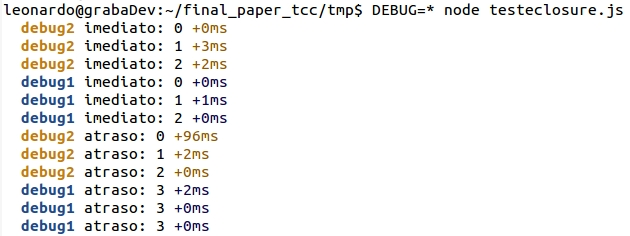
\includegraphics[scale=0.65]{./Resources/call_this.jpg}
	\captionsetup{justification=centering}
	\caption[Resultado de chamada de fun��o sem cria��o de escopo x com cria��o de escopo]{Resultado de chamada de fun��o sem cria��o de escopo x com cria��o de escopo}
	\label{res_call_this}
\end{figure}

\subsection{Servidor Express.js}
\label{servidor_sec}

Mesmo com o servidor Apache configurado por padr�o na BBB, quando foi decidido o uso de Node.js como linguagem do servidor o Apache foi substitu�do pelo \textit{framework} Express, dados os benef�cios apontados na se��o \ref{node_js_sec}. Para isto, a consulta � documenta��o da API deste \textit{framework} (\url{http://expressjs.com/pt-br/4x/api.html}) foi a base de desenvolvimento do servidor. 

Outros dois m�dulos auxiliares foram empregados em conjunto com o Express: o m�dulo \textit{Body-parser}, cuja fun��o neste projeto � a interpreta��o de dados codificados em JSON pelo cliente; e o m�dulo \textit{PHP-express}, que permite a interpreta��o de arquivos PHP pelo servidor. Este �ltimo m�dulo foi empregado devido a algumas funcionalidades desenvolvidas em PHP em uma fase inicial do projeto, portanto suportando a aplica��o legada. Reescrever os c�digos PHP em Javascript � uma op��o, por�m em fun��o do tempo necess�rio para tal tarefa, a solu��o adotada foi executar os c�digos legados. Na caixa \ref{install_express} � documentada a instala��o dos m�dulos Express, \textit{Body-parser} e \textit{PHP-express}.

\lstset{language=bash}
\begin{lstlisting}[frame=single, basicstyle=\linespread{0.85}\ttfamily, caption=Instala��o dos m�dulos necess�rios para implementar o servidor web em Node.js, label=install_express]
npm install express
npm install body-parser
npm install php-express
\end{lstlisting}

O c�digo-fonte no qual � configurado o servidor � o \textit{/var/www/controle.js}, que � tamb�m o arquivo raiz da aplica��o em Node, e est� dispon�vel no ap�ndice \ref{controle_js}. � interessante observar a configura��o do PHP-express, descrita no trecho de c�digo-fonte \ref{php_express}, no qual observa-se que logo ao adicionar o m�dulo ao c�digo � passado o caminho do PHP, que deve estar previamente instalado no sistema. Tamb�m � not�vel o fato de que os arquivos PHP s�o identificados por meio de uma express�o regular, cuja fun��o � qual ela � aplicada direciona estes arquivos para o \textit{engine} do PHP.

\lstset{language=javascript}
\begin{lstlisting}[frame=single, basicstyle=\linespread{0.85}\ttfamily, caption=Configura��o do PHP-express, label=php_express]
var phpExpress = require('php-express')({  // assumes php is in your PATH
  binPath: 'php'
});

// set view engine to php-express
app.set('views', './');
app.engine('php', phpExpress.engine);
app.set('view engine', 'php');
 
// routing all .php file to php-express
app.all(/.+\.php$/, phpExpress.router);
\end{lstlisting}

Com rela��o � configura��o do Express, tr�s pontos devem ser notados: o diret�rio no qual � executada a aplica��o � configurado como o diret�rio raiz do servidor, seja para servir arquivos HTML e CSS ou arquivos de m�dia e apoio da aplica��o; o endere�o de IP e porta s�o especificados de modo a permitir acesso � BBB pela internet e; s�o configuradas rotas para diferentes categorias de requisi��es do cliente. O fragmento de c�digo-fonte \ref{express_server} apresenta os tr�s pontos discutidos neste par�grafo.

\lstset{language=javascript}
\begin{lstlisting}[frame=single, basicstyle=\linespread{0.85}\ttfamily, caption=Configura��o do servidor web com o \textit{framework} Express.js, label=express_server]
var express = require("express");
var app = express();
var routes = require('./my_node_modules/routes.js');

app.use(express.static(__dirname));//add the directory where HTML and CSS files are
var server = app.listen(8587, "192.168.1.155", function () {//listen at the port and address
	var host = server.address().address;
	var port = server.address().port;
	var family = server.address().family;
	debug('Express server listening at http://%s:%s %s', host, port, family);
});

app.route('/controle')//used to unite all the requst types for the same route
.post(routes.controleRoute);

app.route('/startrecipe')//used to unite all the requst types for the same route
.post(routes.startrecipeRoute);

app.route('/config')//used to unite all the requst types for the same route
.post(routes.configRoute);

app.route('/clientrequest')//used to unite all the requst types for the same route
.post(routes.clientrequestRoute);
\end{lstlisting}

Note-se que � adicionado o m�dulo \textit{routes}, que foi escrito separadamente, somente para facilitar a compreens�o do c�digo, embora seja ele que define o comportamento das rotas. Quanto a ele, seu c�digo-fonte � apresentado na caixa de c�digo-fonte do ap�ndice \ref{rotas_js}. Ele consiste de quatro fun��es --- uma para cada rota:

\begin{itemize}
	\item \textbf{controleRoute(req, res)} --- realiza o controle direto de GPIO e PWM. Faz uso do m�dulo \textit{gpio\_cfg}, descrito na se��o \ref{gpio_sec}.
	\begin{itemize}
		\item Muda o valor de um terminal de GPIO ou PWM, conforme especificado pelo cliente.
		\item Retorna para o cliente o status de todos os pinos da aplica��o, independente da sua configura��o.
	\end{itemize}
	\item \textbf{startRecipeRoute(req, res)} --- executa diversas fun��es relacionadas � produ��o de cerveja, inclusive iniciar o processo de controle da mesma, conforme a requisi��o enviada pelo cliente.
	\begin{itemize}
		\item Retorna a lista de receitas cadastradas no servidor.
		\item Verifica integridade de uma receita, ou seja, se ela cont�m informa��es suficientes para que uma produ��o de cerveja seja iniciada.
		\item Realiza uma s�rie de verifica��es e come�a uma brassagem, se aprovado.
		\item Verifica se j� existe alguma receita em andamento.
		\item Retorna erro para o cliente se nenhuma requisi��o � v�lida.
	\end{itemize}
	\item \textbf{configRoute(req, res)} --- ajusta ou responde com a data e hora da BBB, conforme a solicita��o do cliente. S� permite que este ajuste seja realizado se o servi�o de ajuste autom�tico de data/hora n�o estiver funcionando por algum motivo, e.g. problema de conex�o com a internet.
	\item \textbf{clientrequestRoute(req, res)} --- fun��o auxiliar do processo de brassagem, usada para sinalizar que uma nova fase do processo deve come�ar, ap�s autoriza��o do operador/usu�rio.
\end{itemize}

Dentre as particularidades de implementa��o deste m�dulo, observa-se o uso dos argumentos \textit{req} e \textit{res} em todas as fun��es, uma vez que estes s�o padronizado pela API do Express para requisi��es do tipo POST feitas pelo cliente. O argumento \textit{req} cont�m todos os dados enviados pelo cliente no padr�o HTTP POST, que � parte da transfer�ncia de estado representacional, conhecida como REST. Poderia ser o padr�o HTTP GET, por exemplo, por�m neste projeto o POST foi escolhido para que o usu�rio n�o possa adicionar par�metros por meio da URL.

Uma vez que o m�dulo Express est� em conformidade com as restri��es REST, ele � considerado um servi�o \textit{RESTful}. Quanto ao argumento \textit{res}, este cont�m o objeto respons�vel por enviar a resposta do servidor para o cliente ap�s o processamento da requisi��o, que � conseguida por meio m�todo \textit{send}. � importante observar que, neste projeto, todas as requisi��es do cliente e respostas do servidor foram feitas usando a codifica��o de dados JSON. 

O exemplo expresso na caixa de c�digo-fonte \ref{exemplo_reqres} demonstra o uso dos argumentos \textit{req} e \textit{res} descritos nesta se��o. Foi assumido que s�o recebidos os dados \textit{comando} e \textit{valor}. Se o comando for "inverter", � chamada a fun��o que inverte um bot�o, cuja resposta pode ser \textit{erro1} ou \textit{sucesso}. Ainda, se o comando for diferente de "inverter", a resposta � \textit{erro2}.

\lstset{language=javascript}
\begin{lstlisting}[frame=single, basicstyle=\linespread{0.85}\ttfamily, caption=Exemplo de uso dos argumentos \textit{req} e \textit{res} definidos pelo Express.js, label=exemplo_reqres]
function processaRequisicaoPost(req, res) {
	var comando = req.body.comando;
	var botao = req.body.valor;

	if(comando == "inverter"){
		inverteBotao(botao, function(err){
			if (err) res.send('{"resposta":"erro1"}'); return;
			res.send('{"resposta":"sucesso"}');
		});
	}
	else res.send({"resposta":"erro2"});
};
\end{lstlisting}

Tamb�m � importante entender o uso dos m�dulos \textit{fs} e \textit{child\_process} inclu�dos por padr�o no Node.js e cuja documenta��o da API pode ser obtida no site do Node.js (\url{https://nodejs.org/dist/latest-v4.x/docs/api/}). O m�dulo \textit{fs} implementa o acesso ao sistema de arquivos, com fun��es de leitura e escrita a arquivos, mudan�a de dono ou modo de execu��o de arquivos e diret�rios, cria��o e leitura de diret�rios, dentre outras. Quanto � leitura e escrita de arquivos, esta pode ser realizada de forma ass�ncrona ou s�ncrona --- usu�rios que ainda est�o no processo de aprendizado de orienta��o a eventos tendem a usar a vers�o s�ncrona, por�m isto deve ser evitado, uma vez que faz o bloqueio da execu��o da aplica��o enquanto o arquivo n�o acabar de ser acessado.

J� o m�dulo \textit{child\_process} permite a cria��o de processos filhos do Node, que s�o executados independentemente deste: basicamente � poss�vel executar uma linha de comando ou script do \textit{shell} independente do Node. Neste m�dulo, foi utilizada a fun��o \textit{exec} para ajustar a data e hora da BBB ap�s receber uma requisi��o do cliente, por meio dos comandos \textbf{date -s} e \textbf{hwclock -w}, que ajusta a data e hora do sistema e sincroniza com o RTC, respectivamente. A implementa��o desta funcionalidade pode ser verificada na fun��o \textit{configRoute} do c�digo-fonte \ref{rotas_js}, encontrado no ap�ndice \ref{codigos_nodejs}.

\subsection{Registros e verifica��es em geral}
\label{registros_sec}

Para as fun��es de registro, ou \textit{log}, e de verifica��es, al�m de eventuais fun��es de miscel�nea, foi escrito um m�dulo separado, cujo c�digo-fonte est� documentado na caixa \ref{log_check_misc_js} do ap�ndice \ref{codigos_nodejs}. As fun��es e suas respectivas descri��es s�o apresentadas:

\begin{itemize}
	\item \textbf{startTemperatureLogging()} --- inicia o script Python descrito na se��o \ref{python_sec}, por meio de um processo filho do Node.
	\begin{itemize}
		\item Tenta deletar o arquivo que cont�m a �ltima leitura de temperatura (\textit{/var/www/datalog/instant.csv}) antes de iniciar o script em Python.
		\item Define o comportamento caso o script pare de ser executado: imprime uma mensagem de debug.
	\end{itemize}
	\item \textbf{stopTemperatureLogging()} --- aborta a execu��o do script Python iniciado por \textit{startTemperatureLogging}.
	\item \textbf{getTemperatureReading(logFilePath, logReadHandler, callback)} --- l� a mais recente amostragem de temperatura, que est� salva no arquivo especificado pelo argumento \textit{logFilePath}. Al�m da descri��o aqui apresentada, o funcionamento desta fun��o est� descrito no algoritmo da figura \ref{algoritmo_tempread}
	\begin{itemize}
		\item Recebe como argumento uma fun��o de callback padr�o, ou seja, cujo primeiro argumento � o poss�vel erro e o segundo argumento � o valor de temperatura obtido em caso de sucesso.
		\item O argumento \textit{logReadHandler} � um objeto externo � fun��o e que deve guardar o valor da �ltima leitura de temperatura, as �ltimas 5 \textit{timestamps} (registros de data/hora) e a contagem de erros de leitura de temperatura referentes a um sensor espec�fico.
		\item Se h� algum problema na leitura do arquivo que deve conter o registro da �ltima temperatura lida, a vari�vel de erro � incrementada e, se a contagem exceder 180 erros, a mensagem de erro da fun��o de \textit{callback} indica que muitos erros foram detectados. 
		Note-se que 180 � um valor quase que arbitr�rio que pode representar 3 minutos de leituras consecutivas erradas ou 180 erros espor�dicos de leitura do arquivo e cuja escolha foi realizada pois representa 5\% das amostras contidas em uma hora. Esta por sua vez, � aceita como o tempo m�nimo de uma brassagem ou fervura. Testes pr�ticos com rela��o a este aspecto n�o foram realizados, portanto h� espa�o para a realiza��o de ensaios para determina��o de um valor mais adequado.
		\item Em caso de leitura do arquivo com sucesso, se a formata��o do valor lido estiver errada, imprime erro, incrementa a vari�vel de erro e, no caso de a contagem exceder 180, seta a mensagem de erro da fun��o de \textit{callback} indicando que muitos erros foram detectados.
		\item Se o valor lido for consistente, atualiza o objeto \textit{logReadHandler}. Compara as �ltimas 5 \textit{timestamps} obtidas e incrementa a vari�vel de erro se todas elas forem coincidentes --- isto indica primariamente que o sensor de temperatura est� mal conectado, ou mesmo desconectado em caso de erros consecutivos. Por isto a mensagem de erro da \textit{callback} retorna a possibilidade de problemas com o sensor. No caso de a contagem de erros exceder 180, a mensagem de erro da fun��o de \textit{callback} indica que muitos erros foram detectados, ao inv�s de avisar sobre o sensor.
		\item Por fim, se a leitura do registro de temperatura passar por todas as checagens, � retornado nulo na mensagem de erro e o valor de temperatura como segundo argumento.
	\end{itemize}
	\item \textbf{checkRecipeIntegrity(recipe, path, res)} --- Verifica a integridade da receita selecionada pelo usu�rio antes de permitir o in�cio de uma brassagem. Os argumentos recebidos pela fun��o s�o o nome da receita, o diret�rio de receitas a ser verificado e o objeto que cont�m a resposta da requisi��o AJAX feita pelo cliente, respectivamente.
	\begin{itemize}
		\item Se n�o consegue ler o arquivo da receita, responde com erro ao cliente.
		\item Caso contr�rio, l� o arquivo \textit{lockfile} para verificar se j� existe uma brassagem em andamento. Se n�o consegue ler o \textit{lockfile} ou ele indica que h� uma brassagem em andamento, tamb�m responde com erro.
		\item Verifica a consist�ncia da receita com o seguinte crit�rio: h� campos estritamente necess�rios para a produ��o e que impedem o in�cio da receita se estiverem em branco, campos que geram avisos mas permitem o in�cio de uma receita ap�s o usu�rio se declarar ciente e campos indiferentes para o sistema. S�o os campos estritamente necess�rios: �gua de brassagem, tempo da fervura, temperatura inicial de brassagem, primeiro degrau de temperatura, tempo do primeiro degrau, malte 1, quantidade do malte 1, l�pulo 1, quantidade do l�pulo 1 e tempo de adi��o do l�pulo 1. Os campos que geram avisos s�o: nome da receita, estilo, levedura, �gua de sparging e temperatura de sparging. Todos os outros campos s�o indiferentes � verifica��o de consist�ncia.
		\item Se tudo deu certo, uma vari�vel global � setada para registro e uso posterior.
	\end{itemize}
\end{itemize}

\begin{figure}[H]
	\centering
	\includegraphics[scale=0.55]{./Resources/algoritmo_tempread.png}
	\captionsetup{justification=centering}
	\caption[Representa��o em fluxograma do algoritmo de implementa��o da fun��o \textit{getTemperatureReading}]{Representa��o em fluxograma do algoritmo de implementa��o da fun��o \textit{getTemperatureReading}}
	\label{algoritmo_tempread}
\end{figure}

\begin{itemize}
	\item \textbf{logToFile(message, code, notableTimestamp)} --- fun��o que realiza registro do status da brassagem sempre que invocada. Basicamente, ela salva a vari�vel global \textit{environmentVariables} em um arquivo de texto.
	\begin{itemize}
		\item O argumento \textit{message} pode conter uma string com uma mensagem explicativa contendo, por exemplo, a situa��o ou est�gio da brassagem em que ocorreu o registro, mas pode tamb�m ser deixado em branco. O argumento \textit{code} tem basicamente o mesmo prop�sito, mas � um n�mero predefinido para cada situa��o poss�vel da brassagem, que permite que o arquivo de registro possa ser interpretado com maior facilidade; por este motivo, recomenda-se veementemente que n�o seja deixado em branco. A tabela \ref{significados_log} apresenta a correspond�ncia entre os valores do argumento \textit{code} e seus significados.
		\item O argumento \textit{notableTimestamp} � usado para indicar quando uma situa��o not�vel ocorreu, como por exemplo o in�cio da brassagem, o final de uma rampa ou degrau de temperatura, o in�cio da fervura, etc. Para todas as outras situa��es deve ser deixado em branco, sendo que as situa��es not�veis s�o predefinidas.
		\item O objeto \textit{environmentVariables}, declarado no c�digo-fonte raiz da aplica��o em Node, que foi abordado na se��o \ref{servidor_sec} e pode ser obtido no ap�ndice \ref{codigos_nodejs}, tamb�m � descrito na caixa \ref{environment_code}. Ele � salvo no arquivo de \textit{log} no formato JSON e para isto � empregada a fun��o \textit{JSON.stringify} conforme descrito na linha de c�digo-fonte exibida na caixa \ref{json_stringify}.
	\end{itemize}
	\item \textbf{sendRecipeNames(path, res)} --- responde para o cliente usando o objeto \textit{res} com todas as receitas dispon�veis no diret�rio passado como argumento \textit{path} para a fun��o.
	\begin{itemize}
		\item � preciso notar que, quando uma receita � deletada, a �nica modifica��o realizada � que a extens�o do arquivo \textit{.recipe} � modificada para \textit{.recipe.del}, assim � f�cil recuperar a receita caso o usu�rio a tenha deletado por engano. Por isso nesta fun��o, al�m de ler os nomes dos arquivos presentes no diret�rio e excluir a extens�o, foi preciso ignorar os arquivos deletados.
	\end{itemize}
\end{itemize}

\lstset{language=javascript}
\begin{lstlisting}[frame=single, basicstyle=\linespread{0.85}\ttfamily, caption=Declara��o do objeto \textit{environmentVariables}, que cont�m o status instant�neo da brassagem, label=environment_code]
//global variables that should also be saved to a backup file periodically
global.environmentVariables = {
	warn: "",//if not empty holds some warning message
	code: "",//tells the same as msg, but as an index, easier to check programatically
	tmpMT: "",//mash tun temperature
	tmpMTsetp: "",//mash tun current setpoint
	tmpBK: "",//brewing kettle temperature, also the "hot liquor tank" for sparging
	tmpBKsetp: "",//brewing kettle/hot liquor tank current setpoint
	timeLeft: "",//helping variable to tell the client the time left for the step rests or the boil, etc
	readyForNextStep: false,//set whenever the system is ready for the next step
	auto: true, //whether the process control is running automatically or there is human intervention
	processFail: false,//flag is set if the process fails irreversibly
	msg: "",//holds some explanatory message
	timestamps:{//notable timestamps
		curr: "",//epoch time of the current variables state
		start: "",//epoch time of the first request to start a recipe
		startHeating: "",//epoch time of the start to heat the mash water
		finishHeating: "",//epoch for the finish of the heating of mash water
		//start of the ramps
		sRamp0: "", sRamp1: "", sRamp2: "", sRamp3: "", sRamp4: "", sRamp5: "", sRamp6: "", sRamp7: "",
		//finish of the ramps
		fRamp0: "", fRamp1: "", fRamp2: "", fRamp3: "", fRamp4: "", fRamp5: "", fRamp6: "", fRamp7: "",
		startDrain: "",//start of the sparging process, when the mash is parcially drained to the BK
		startSparge: "",//here the recirculation pump starts working
		heatingBoil: "",//started to heat the wort after sparging
		boilStart: "",//time when temperature is near enough boiling (>96�C)
		//hop additions
		hAdd0: "", hAdd1: "", hAdd2: "", hAdd3: "", hAdd4: "", hAdd5: "", hAdd6: "", hAdd7: "", 
		boilFinishScheduled: "",//time when the boil is scheduled to finish
		chillStart: "",//time when the the boil really finishes and the chilling starts
		end: "",//epoch time of the end of the brewing (there is cleaning after it)
		cleaningStart: "",//when the cleaning recirculation process starts
	},
	ioStatus: gpioCfg.all_io,//also records the IO status
	okToStart: false, //true if a recipe is ok enough to start a production
	recipe: "" //recipe name
};
\end{lstlisting}

\lstset{language=javascript}
\begin{lstlisting}[frame=single, basicstyle=\linespread{0.85}\ttfamily, caption=Uso da fun��o \textit{JSON.stringify} para codificar um objeto em string JSON, label=json_stringify]
dataToSave = JSON.stringify(global.environmentVariables) + "\n";
\end{lstlisting}

\begin{center}
	\begin{table}[H]
		\centering
		\captionsetup{justification=centering}
		\caption[Correspond�ncia entre o valor num�rico e o significado dos c�digos usados para registro da brassagem]{Correspond�ncia entre o valor num�rico e o significado dos c�digos usados para registro da brassagem}
		\label{significados_log}
		\begin{tabular}{ | M{2cm} | M{13cm} |}
			\hline
			\textbf{Valor} & \textbf{Significado} \\ \hline
			
			0 & requisi��o para in�cio da brassagem \\ \hline
			1 & produ��o iniciada \\ \hline
			2 & esquentando �gua da mostura \\ \hline
			3 & esperando adi��o dos gr�os \\ \hline
			4 & rampa da mostura em execu��o \\ \hline
			5 & degrau da mostura em execu��o \\ \hline
			6 & \textit{sparging} em execu��o \\ \hline
			7 & transbordamento da MT \\ \hline
			8 & esquentando mosto para a fervura \\ \hline
			9 & fervendo o mosto \\ \hline
			10 & l�pulo adicionado \\ \hline
			11 & resfriando o mosto\\ \hline
			12 & fim do resfriamento, esperando OK do operador para limpeza\\ \hline
			13 & recircula��o de �gua para limpeza\\ \hline

		\end{tabular}
	\end{table}
\end{center}

\subsection{Controle do processo de brassagem}

O m�dulo respons�vel pelo controle do processo de brassagem � o \textit{ctrl.js}, cujo c�digo-fonte est� dispon�vel no ap�ndice \ref{codigos_nodejs}, na caixa de c�digo-fonte \ref{ctrl_js}. � importante ressaltar que, embora o comportamento do Node.js seja ass�ncrono o processo de brassagem � sequencial, o que implica no uso de diversas fun��es de \textit{callback} aninhadas. No intuito de evitar o \textit{inferno de callbacks}, apresentado na se��o \ref{node_js_sec}, este processo sequencial foi quebrado em algumas fun��es que implementam a funcionalidade do m�dulo e outras auxiliares. Seu funcionamento e aspectos chave s�o discutidos na presente se��o.

\subsubsection{In�cio do processo}

A primeira fun��o do processo de controle � a \textit{startMashingProcess(recipe, res, lockFile, recipesPath, callback)}, invocada a partir de uma requisi��o do cliente e, portanto, sua chamada est� presente no m�dulo referente �s rotas do Express, discutido na se��o \ref{servidor_sec}. Ela recebe como par�metros o nome da receita a ser iniciada, o objeto de resposta da requisi��o AJAX, o caminho para o arquivo \textit{lockfile}, o caminho para o diret�rio das receitas e uma fun��o de \textit{callback}. Em primeiro lugar � verificada a flag global \textit{global.environmentVariables.okToStart} que indica se a receita est� pronta para ser executada --- esta flag � setada previamente pela fun��o \textit{checkRecipeIntegrity}, descrita na se��o \ref{registros_sec} e chamada durante o processo de intera��o pr�-brassagem do usu�rio com o sistema. Depois disto, tamb�m � verificado se o nome da receita passado como argumento � id�ntico ao da vari�vel global de controle \textit{global.environmentVariables.recipe}.

Caso as verifica��es iniciais sejam positivas, � escrito o valor "1" no arquivo \textit{lockfile}, indicando daqui para a frente que h� uma brassagem em andamento. O conte�do da receita � lido em uma vari�vel e o \textit{log} de temperatura � iniciado, ou seja, o script Python � invocado como um processo filho do Node. Tamb�m � feito o \textit{log} inicial do processo de brassagem. Se tudo ocorreu sem erros, o servidor envia uma resposta para o cliente indicando sucesso, chama a fun��o de \textit{callback} com a vari�vel \textit{erro} nula e invoca a fun��o \textit{heatMashWater}, que d� prosseguimento ao controle do processo. Em caso de erro em alguma das situa��es descritas, � enviada uma resposta de erro para o cliente e a fun��o de \textit{callback} � invocada com a vari�vel erro indicando o erro ocorrido. Note-se que a fun��o de \textit{callback} n�o tem import�ncia no que diz respeito ao controle, mas serve somente para retornar o status da tentativa de in�cio da produ��o.

\subsubsection{Aquecimento da �gua da mostura}

A fun��o \textit{heatMashWater(recipeContents)} rec�m chamada, d� prosseguimento ao controle da brassagem. Como o seu nome sugere, ela � respos�vel pelo aquecimento da �gua da brassagem at� que seja atingida a temperatura inicial, mantendo este \textit{setpoint} at� que o usu�rio adicione os maltes � MT. O �nico argumento que a fun��o recebe � o conte�do da receita, a partir do qual � obtido o \textit{setpoint}. Inicialmente a bomba de recircula��o � ligada e � feito um \textit{log} da brassagem que anota a timestamp not�vel de inicio de aquecimento.

S�o iniciados dois la�os de repeti��o: um que faz um \textit{log} da situa��o da brassagem a cada 5 segundos e outro que � repetido a cada 1 segundo e que l� a temperatura da �gua e chama a fun��o auxiliar \textit{updateHeatingConditions} para controlar o elemento aquecedor da MT. No \textit{callback} da \textit{updateHeatingConditions} fica definido que, se esta � a primeira vez que a temperatura desejada � atingida, o la�o de repeti��o do \textit{log} � atualizado para refletir a mudan�a de situa��o de "esquentado �gua da brassagem" para "esperando adi��o dos maltes". Se n�o � a primeira vez que � atingido o \textit{setpoint}, a \textit{callback} n�o faz nada. Em resumo, ap�s a temperatura atingir o valor desejado, ela � mantida at� que o usu�rio adicione os maltes.

Concomitantemente, o la�o de controle de temperatura da fun��o \textit{heatMashWater} verifica a \textit{flag} global \textit{global.environmentVariables.readyForNextStep} que s� � setada ap�s o usu�rio indicar, por meio da GUI, que ele adicionou os maltes. Quando isto acontece, a flag � zerada e os la�os de \textit{log} e de controle s�o interrompidos. Por fim � chamada a fun��o de controle de rampas e degraus de temperatura, mas antes de entrar nos seus detalhes de funcionamento, ser� explicada a fun��o auxiliar \textit{updateHeatingConditions(vessel, setp, temperature, callback)}.

\subsubsection{Fun��o de controle de temperatura}

Os argumentos que ela recebe possuem uma interpreta��o bem direta: \textit{vessel} � o recipiente a ser controlado, ou seja, pode ser a MT ou o BK; \textit{setp} e \textit{temperature} s�o respectivamente a temperatura desejada e a atual e; \textit{callback} � a fun��o executada sempre que a temperatura � maior ou igual ao valor do setpoint, e cujo argumento passado para ela � nulo. O controle do elemento aquecedor � implementado da seguinte forma: quando a temperatura est� abaixo de 70\% do \textit{setpoint}, o aquecimento fica ligado 100\% do tempo; quando a temperatura est� entre 70\% e 90\% do \textit{setpoint}, o aquecimento fica ligado 66\% do tempo; quando a temperatura est� entre 90\% e 100\% do \textit{setpoint}, o aquecimento fica ligado 33\% do tempo e; acima disto o aquecimento fica desligado.

Cabe ressaltar que a vantagem desta fun��o auxiliar n�o � o sistema de controle de aquecimento, mas sim o fato de que este � auto-contido, ou seja, para quaisquer implementa��es de controle de temperatura (PID, histerese, direto), basta modificar esta fun��o, sem altera��o do resto do c�digo. Outra condi��o que deve ser atendida � que esta fun��o precisa ser chamada periodicamente dentro de um la�o de repeti��o, uma vez que ela somente atualiza o valor da sa�da (elemento aquecedor) baseada nas entradas (temperatura e \textit{setpoint}).

\subsubsection{Controle de rampas e degraus de temperatura}

De volta ao fluxo de controle da produ��o, ap�s o usu�rio adicionar os maltes, a fun��o \textit{rampControl(recipeContents)} � chamada. Ela recebe somente o conte�do da receita, a partir do qual s�o obtidas as temperaturas e tempos dos degraus de repouso da mostura, assim como a temperatura da �gua de \textit{sparging}. Se a temperatura de \textit{sparging} n�o estiver definida, � assumido que esta parte do processo deve ser omitida. Depois desta verifica��o � feito um log indicando in�cio de rampa de temperatura e � iniciado um \textit{loop} no qual � registrada a situa��o da brassagem a cada 5 segundos. 

\newpage

Em paralelo, outro la�o de repeti��o implementa a parte relativa ao controle: se ainda h� a possibilidade de mais degraus de temperatura, esta � verificada:

\begin{itemize}
	\item Em caso positivo, os valores do degrau e temperatura s�o obtidos, o \texit{loop} de registro � atualizado e o controle do pr�ximo degrau � iniciado
	\item Em caso negativo isto siginifica que esta parte do processo acabou e � sinalizado que a fervura/\texit{sparging} deve come�ar.
\end{itemize}

Se o processo de fervura/\texit{sparging} deve come�ar, os resistores de aquecimento da MT e do BK s�o desligados, assim como a bomba de recircula��o da MT. Os la�os de registro e controle s�o interrompidos e a fervura ou a lavagem � iniciada, dependendo da verifica��o feita anteriormente quanto ao \textit{setpoint} da vari�vel de sparging.

Se a etapa de rampas e degraus ainda n�o acabou, a temperatura da MT � lida e o la�o de controle de temperatura � executado, usando a fun��o \textit{updateHeatingConditions}. Ainda, caso haja �gua de lavagem para esquentar, o resistor de aquecimento do BK � ligado sempre que o resistor de aquecimento da MT estiver desligado. Ambos os resistores de aquecimento s�o impedidos de ligar ao mesmo tempo pois o sistema el�trico foi dimensionado para operar com corrente m�xima referente a um resistor em opera��o.

\subsubsection{Lavagem dos gr�os}

A fun��o de controle da lavagem dos gr�os � fortemente baseada em temporiza��o: o fluxo de vaz�o da MT para o BK e o fluxo de bombeamento de l�quido do BK para a MT devem ser iguais para que n�o ocorra transbordamento de nenhum dos recipientes, mas como na pr�tica estes fluxos s�o muito diferentes e variam conforme a receita, o ideal seria o projeto de dispositivos de verifica��o de transbordamento da panela.

� iniciado um la�o de registro da situa��o da brassagem a cada 5 segundos e, em paralelo, outro la�o executado a cada 0,5 segundos verifica se h� transbordamento da MT. Em caso afirmativo, a bomba do BK � desligada e um tempo predefinido � esperado at� que o bombeamento seja retomado. Em paralelo aos dois la�os de repeti��o, a v�lvula de drenagem da MT � inicialmente aberta por um tempo determinado em fun��o do volume inicial da �gua de brassagem, definido como $0,5 segundos \cdot volume(l)$. Somente quando este tempo acaba � que � a valvula de drenagem e a bomba de recircula��o do BK s�o ativadas, para iniciar a lavagem dos gr�os; tamb�m � neste momento que � iniciado um terceiro \textit{loop}.

\newpage

Neste, executado a cada 0,5 segundos, nada acontece em caso de transbordamento. Se tudo estiver ocorrendo conforme planejado, este la�o espera um tempo baseado no volume da �gua de lavagem, definido como $3 segundos \cdot volume(l)$. Depois que este tempo acaba, � feita a drenagem completa da MT, todos os la�os de repeti��o s�o interrompidos e � dado in�cio ao processo de fervura.

\subsubsection{Fervura}

A fun��o \textit{theBoil(recipeContents)} recebe somente o conte�do da receita. � iniciado um la�o de registro da brassagem a cada 5 segundos e em paralelo, ap�s ligar o resistor de aquecimento do BK, � iniciado um la�o supervisor da fervura executado a cada 1 segundo e no qual s�o controladas as adi��es de l�pulos. Neste la�o, s� � iniciada a contagem do tempo de fervura depois que a temperatura do mosto sobe al�m dos 96\si{\degree}C, momento no qual tamb�m � atualizado o la�o de registro e s�o agendadas para execu��o as adi��es dos l�pulos por meio da fun��o \textit{setTimeout}. Quando a fervura acaba, � desligado o resistor de aquecimento do BK, fechado o compartimento de adi��o de l�pulos e interrompidos os la�os de registro e supervis�o da fervura.

\subsection{Simula��o do controle do processo de brassagem}
\label{simulacao_controle}

Para testar o c�digo de controle, foi utilizada a fun��o \textit{tlog\_test} do script Python de log de temperaturas, apresentada na se��o \ref{python_sec}. Com isto, foi poss�vel usar a interface web para executar o processo de controle de brassagem como operador do sistema, usando uma receita de cerveja especificamente criada para o prop�sito de \textit{debug}, j� que uma receita de verdade tem dura��o de mais de duas horas, tempo elevado para teste de c�digo. As caracter�sticas da receita s�o apresentadas na tabela \ref{receita_debug}. Par�metros porventura omitidos significam que estes foram deixados em branco ao preencher a receita na interface web.

\begin{center}
	\begin{table}[H]
		\centering
		\captionsetup{justification=centering}
		\caption[Par�metros de receita de cerveja utilizados para \textit{debug}]{Par�metros de receita de cerveja utilizados para \textit{debug}}
		\label{receita_debug}
		\begin{tabular}{ | M{13cm} | M{2cm} |}
			\hline
			\textbf{Par�metro} & \textbf{Valor} \\ \hline
			
			Nome & Quick Response Debug \\ \hline
			Estilo & no style \\ \hline
			�gua mostura��o & 30 litros\\ \hline
			�gua \textit{sparging} & 20 litros \\ \hline
			Temperatura \textit{sparging} & 50\si{\degree}C \\ \hline
			Fervura do mosto & 5 minutos \\ \hline
			Malte 1 & no malts \\ \hline
			Quantidade malte 1 & 1 kg \\ \hline
			L�pulo 1 & hop 1 \\ \hline
			Quantidade l�pulo 1 & 1 g \\ \hline
			Tempo de adi��o 1 & 1 minuto \\ \hline
			L�pulo 2 & hop 2 \\ \hline
			Quantidade l�pulo 2 & 1 g \\ \hline
			Tempo de adi��o 1 & 4 minutos \\ \hline
			L�pulo 3 & hop 3 \\ \hline
			Quantidade l�pulo 3 & 1 g \\ \hline
			Tempo de adi��o 3 & 2 minutos \\ \hline
			Temperatura inicial & 30\\ \hline
			Temperatura 1 & 35\si{\degree}C\\ \hline
			Tempo 1 & 1 minuto\\ \hline
			Temperatura 2 & 40\si{\degree}C\\ \hline
			Tempo 2 & 0 minutos\\ \hline
		\end{tabular}
	\end{table}
\end{center}


%%%%%%%%%%%%%%%%%%%%%%%%%%%%%%%%%%%%%%%%%%%%%%%%%%%%%%%%%%%%%%%%%%%%%%%%%%

\section{Interface de usu�rio}
A interface de usu�rio foi desenvolvida para acesso via navegador da internet, em um computador com tela de resolu��o WXGA (1366 x 768 pixels). As linguagens utilizadas para a implementa��o da aplica��o foram: a linguagem de marca��o HTML, a linguagem de folhas de estilo CSS, a linguagem de programa��o \textit{client-side} interpretada Javascript em conjunto com a biblioteca \textit{crossbrowser} jQuery e o m�todo AJAX, a linguagem de programa��o \textit{server-side} interpretada PHP e, a linguagem de programa��o \textit{server-side} Javascript interpretada pela aplica��o Node.js.

\subsection{Aspectos gerais da GUI}
\label{aspectos_sec}

A estrutura da aplica��o foi desenvolvida de forma que o operador do sistema conseguisse tanto gerenciar suas receitas de cerveja e analisar dados estat�sticos de maneira f�cil, quanto para promover a comunica��o eficiente entre o cliente e o servidor, implementado em Node.js e discutido na se��o \ref{nodectrl_sec}. A estrutura da aplica��o do cliente � apresentada:

\begin{itemize}
	\item P�gina inicial
	\item Sobre
	\item Configura��es
	\item Estat�sticas
	\item Iniciar brassagem
	\begin{itemize}
		\item Controle de brassagem
	\end{itemize}
	\item Gerenciador de receitas
	\begin{itemize}
		\item Editor de receitas
	\end{itemize}
\end{itemize}

Um ponto em comum para esta estrutura, com exce��o da p�gina inicial, foi o desenvolvimento de uma barra de navega��o em PHP, cujo c�digo-fonte est� documentado na caixa \ref{header_php} do ap�ndice \ref{codigos_web}, de tal modo que o mesmo c�digo-fonte pudesse ser reaproveitado para todas as p�ginas web. A implementa��o consistiu na cria��o de uma estrutura de \textit{divs} e \textit{links} em HTML, sendo que a fun��o detecta a p�gina atual e real�a este link, para dar ao usu�rio um efeito visual de que certo bot�o da barra de navega��o est� pressionado. 

� usada uma fun��o em javascript, descrita na caixa de c�digo-fonte \ref{js_php_header} e tamb�m no ap�ndice \ref{codigos_web}, que faz a ponte entre PHP e javascript, j� que o servidor Express n�o foi configurado para suportar as vari�veis \textit{http\_host} e \textit{request\_uri} --- assim sendo, a fun��o passa a URL da p�gina atual para o script PHP por meio de um POST HTTP em AJAX.

\lstset{language=javascript}
\begin{lstlisting}[frame=single, basicstyle=\linespread{0.85}\ttfamily, caption=Fun��o que passa a URL da p�gina atual para um m�dulo em PHP, label=js_php_header]
function headerPHP(pathToHeader){//create the header of the page
    $.post(pathToHeader, {url:document.URL} , function(data, status){//send the page URL to PHP
        if(status == "success"){//if POST is successfull
            $('body').prepend($(data));//add the received header to the top of the page
            $('body').show();//and displays the hidden page afterwards
        }
    });
}
\end{lstlisting}

Com rela��o ao estilo do template desenvolvido para toda a GUI, este � documentado nos c�digos-fonte CSS \ref{css_form}, \ref{css_buttons} e \ref{css_config} do ap�ndice \ref{codigos_web}. O processo de cria��o do template foi iterativo e dependente das funcionalidades a serem implementadas, mas n�o seguiu uma lista de tarefas ou algo similar; do contr�rio, seu desenvolvimento foi realizado em conjunto com o resto da interface web.

\subsection{Boas vindas e informa��es do projeto}

A \textit{p�gina inicial} cont�m somente uma mensagem de boas vindas clic�vel, que leva para a p�gina \textit{sobre}. Esta por sua vez, cont�m informa��es sobre o projeto: objetivo, local, autor, professor orientador e contato. Ambos os c�digos-fonte est�o inclusos respectivamente nas caixas \ref{index_html} e \ref{about_php} do ap�ndice \ref{codigos_web}.

\subsection{Configura��es gerais da BBB}

A p�gina \textit{configura��es} apresenta a data/hora da BBB com taxa de atualiza��o de 1 segundo e permite o seu ajuste, para que o usu�rio tenha uma alternativa caso a configura��o de data/hora autom�tica falhe ou n�o exista acesso � internet naquele momento. A obten��o de um valor de data/hora introduzido pelo usu�rio do sistema utiliza o campo de formul�rio \textit{datetime-local} do padr�o HTML5, que implementa automaticamente um calend�rio para escolha da data e devolve a entrada do usu�rio de acordo com o padr�o ISO 8601, cujo formato � apresentado na tabela \ref{iso_8601}. A letra T da string delimita a separa��o entre data e hora e a letra Z indica que o fuso hor�rio � o UTC 0, tamb�m conhecido como GMT. 

\begin{center}
	\begin{table}[H]
		\centering
		\captionsetup{justification=centering}
		\caption[Padr�o de data/hora no formato ISO 8601]{Padr�o de data/hora no formato ISO 8601}
		\label{iso_8601}
		\begin{tabular}{ | M{15cm}|}
			\hline
			AAAA-MM-DDTHH:MM:SSZ \\ \hline
			2016-05-07T18:31:53Z \\ \hline
		\end{tabular}
	\end{table}
\end{center}

Tanto a obten��o da data da BBB quanto a requisi��o para sua mudan�a foram implementadas por meio de requisi��es AJAX para a rota \textit{config} do servidor. Cabe salientar que s� � permitido ao usu�rio mudar a configura��o de data/hora do sistema se o servidor identificar que o servi�o de ajuste autom�tico \textit{ntp} n�o estiver funcionando.

\subsection{Estat�sticas e gr�fico din�mico}

A p�gina \textit{estat�sticas} apresenta a temperatura instant�nea da MT, um gr�fico din�mico da temperatura da MT e do BK que � atualizado automaticamente e um gr�fico do hist�rico de temperatura, plotado usando o script Python desenvolvido na se��o \ref{python_graph}. O gr�fico din�mico foi desenvolvido em uma p�gina separada e posteriormente adicionado como um \textit{iframe}, ou seja, uma p�gina HTML dentro de outra p�gina HTML. Seu c�digo-fonte est� dispon�vel na caixa \ref{stats_php} do anexo \ref{codigos_web}.

O gr�fico din�mico foi baseado na biblioteca D3.js, escrita em Javascript e voltada para a manipula��o de documentos baseados em dados, em conjunto com o \textit{framework} Rickshaw para plotagem de gr�ficos. A instala��o da biblioteca D3.js consistiu no download do arquivo compactado e posterior extra��o, enquanto para o Rickshaw bastou clonar o reposit�rio do Github. Os passos executados est�o descritos na caixa \ref{install_d3}.

\lstset{language=bash}
\begin{lstlisting}[frame=single, basicstyle=\linespread{0.85}\ttfamily, caption=Instala��o da biblioteca D3.js e do framework Rickshaw, label=install_d3]
cd /var/www
https://github.com/mbostock/d3/archive/v3.5.10.zip
sudo tar -zxvf v3.5.10.tar.gz
sudo rm v3.5.10.tar.gz
sudo git clone https://github.com/shutterstock/rickshaw.git
\end{lstlisting}

O gr�fico implementado � baseado em um exemplo dispon�vel em \url{https://github.com/shutterstock/rickshaw/blob/master/examples/extensions.html} e o c�digo-fonte empregado neste projeto est� dispon�vel na caixa \ref{dyn_html} do anexo \ref{codigos_web}. Suas possibilidades de configura��o pelo usu�rio s�o:

\begin{itemize}
	\item Possibilidade a sele��o de quais conjuntos de dados plotar
	\item Op��o de plotagem em �rea empilhada/sobreposta ou em linha
	\item Liga��o dos pontos de maneira interpolada, que suaviza transi��es bruscas e descontinuidades; linear, que liga os pontos diretamente ou; em degrau, que tra�a uma linha horizontal e outra vertical entre dois pontos
	\item Possibilidade de aplicar um filtro de suaviza��o com intensidade ajust�vel (filtro de m�dias m�veis);
	\item Escolha do n�mero m�ximo de pontos plotados na tela --- 300, 1800 ou 3600 pontos
	\item Barra de zoom
\end{itemize}

As caracter�sticas de plotagem dos gr�ficos consistema na escala e numera��o autom�tica dos eixos, incluindo escala baseada no tempo Epoch, e na possibilidade de obter informa��es detalhadas sobre um ponto do gr�fico ao posicionar o cursor sobre ele: valor do ponto e sua respectiva data/hora.

Exceptuando-se o controle do n�mero m�ximo de pontos, que foi implementado para limitar a 300, 1800 e 3600 pontos, e a atualiza��o constante do gr�fico, implementados separadamente para este projeto, todas as outras funcionalidades foram baseadas nas fun��es do Rickshaw. Um aspecto importante da implementa��o do gr�fico foi que, ao carregar a p�gina web, � feita a leitura do arquivo CSV com o registro do hist�rico de temperatura, por�m quando � feita a atualiza��o deste hist�rico, � lido o arquivo CSV que cont�m somente a �ltima leitura de temperatura, com o objetivo de n�o sobrecarregar tanto o cliente quanto o servidor com a troca e processamento de dados redundantes. Com rela��o � temperatura instant�nea, � este gr�fico din�mico que a fornece para a p�gina m�e \textit{estat�sticas} a cada 1 segundo, que por sua vez repassa para o seu elemento HTML correspondente.

\subsection{Gerenciador de receitas}
\label{gerenciador_sec}

A interface do gerenciador de receitas foi programada para apresentar as seguintes op��es e funcionalidades: criar uma nova receita; editar ou apagar uma receita j� cadastrada e; obter uma pr�via de determinada receita ao repousar o mouse sobre seu nome.

Para listar as receitas do diret�rio \textit{www/recipes} foi usada uma fun��o em PHP escrita diretamente no c�digo-fonte da p�gina web, que est� dispon�vel na caixa \ref{listrecipe_php} do ap�ndice \ref{codigos_web}. Deve-se notar que esta fun��o, al�m de excluir a extens�o \textit{.recipe} do nome dos arquivos de receitas, substitui todos os caracteres \textit{underline} por espa�os, uma vez que ao salvar a receita o processo inverso � realizado. Ela adiciona as receitas � lista apresentada ao usu�rio no formato de um link para cada receita, sendo que estes, por sua vez, redirecionam o usu�rio para a p�gina de edi��o de receitas quando clicados. Ao lado de cada link, tamb�m � dinamicamente adicionado um bot�o para deletar a receita correspondente.

Em javascript, foram implementadas as funcionalidades de pr�via de determinada receita a partir das fun��es \textit{mouseover} e \textit{mouseout} da biblioteca jQuery. Al�m disto, tamb�m foram implementadas as fun��es para deletar e criar receitas. Note-se que as fun��es que deletam receitas e geram pr�via foram implementadas em um arquivo separado ao do c�digo HTML, e que est� apresentado na caixa de c�digo-fonte \ref{listrecipe_js} do ap�ndice \ref{codigos_web}.

Ambas as fun��es do m�dulo adicional usam a requisi��o HTTP POST, implementada por meio do m�todo AJAX, para comunica��o com o servidor. Especificamente para a fun��o que deleta receitas, sua implementa��o possibilitou ao usu�rio desfazer a a��o em caso de clique acidental. Mesmo quando o clique n�o � acidental, a implementa��o foi realizada de tal forma que a receita n�o � realmente deletada da BBB, mas somente adicionada a extens�o \textit{.del} ao nome do arquivo.

\subsection{Editor de receitas}
\label{recipe_editor_howto}

O editor de receitas foi uma das primeiras p�ginas acresentadas � GUI, portanto grande parte do gerenciamento do formul�rio HTML que foi implementado � realizado em PHP. Dentre as funcionalidades, est�o a adi��o de novos campos de maltes, l�pulos e temperaturas � medida que o usu�rio preenche a receita; a verifica��o dos dados inseridos para que o usu�rio n�o adicione entradas com caracteres especiais ou diferentes do esperado (e.g. usu�rio escrever letras em um campo no qual s�o esperados n�meros); a verifica��o e aviso ao usu�rio de que h� campos importantes n�o preenchidos; a reordena��o dos campos quando o usu�rio apaga um malte, l�pulo ou temperatura e; o salvamento autom�tico da receita na BBB.

O editor de receitas est� dividido em tr�s c�digos-fonte dispon�veis no ap�ndice \ref{codigos_web}: o c�digo HTML, que s� implementa o esqueleto da p�gina e chama as fun��es dos outros arquivos, apresentado na caixa \ref{newrecipe_code}; um m�dulo com fun��es implementadas em javascript, apresentado na caixa \ref{newrecipe_code_js}; e um m�dulo com fun��es implementadas em PHP, apresentado na caixa \ref{newrecipe_code_php}.

No c�digo HTML, ao carregar a p�gina web, foi inclu�do o m�dulo PHP e chamada uma fun��o que verifica se foi recebida uma receita pela URL, por meio do m�todo GET. Somente em caso afirmativo � que uma fun��o l� o conte�do da receita em um arranjo e a retorna para a p�gina HTML, que por sua vez carrega os dados no formul�rio. Ap�s isto, foi implementado um trecho de c�digo javascript que organiza os campos da receita caso existam buracos. Por exemplo: se o malte 1 e o malte 3 est�o cadastrados mas n�o h� malte 2, o c�digo javascript trata de reorganizar o malte 3 para malte 2. Em seguida foi obtido o nome da receita a partir da URL, e por fim chamada uma fun��o toda vez que algum campo do formul�rio perde o foco, que implementa o rearranjo dos campos se necess�rio e faz o \textit{autosave} da receita.

No m�dulo escrito em javascript, � interessante o funcionamento da fun��o recursiva que reorganiza os campos do formul�rio, cuja assinatura � \textit{rearrange(catg, line)}, sendo o argumento \textit{catg} o indicador de quais campos devem ser reorganizados (maltes, l�pulos ou degraus de temperatura) e \textit{line} o argumento que indica a partir de qual linha deve ser feita a ordena��o. O par�metro line deve ser zero ou omitido na primeira vez que a fun��o � invocada, j� que ela atribui o valor zero no caso de este par�metro ser indefinido. O algoritmo de implementa��o est� descrito no fluxograma da figura \ref{rearrange}.

\begin{figure}[H]
	\centering
	\includegraphics[scale=0.36]{./Resources/rearrange.png}
	\captionsetup{justification=centering}
	\caption[Representa��o em fluxograma do algoritmo de implementa��o da fun��o \textit{rearrange}]{Representa��o em fluxograma do algoritmo de implementa��o da fun��o \textit{rearrange}}
	\label{rearrange}
\end{figure}

\subsection{Gerenciador de brassagem}

A interface que controla o andamento de uma produ��o, cujo c�digo-fonte est� descrito na caixa \ref{startrecipe_code} do anexo \ref{codigos_web} apresentou uma interface inicial que permitiu ao usu�rio do sistema selecionar a receita alvo da produ��o e inici�-la. � preciso notar, por�m, que a primeira fun��o executada faz uma requisi��o para o servidor perguntando se h� uma receita j� em andamento: em caso positivo, a p�gina � redirecionada para o painel de controle das receitas, descrito na se��o \ref{painel_sec}, impedindo portanto o usu�rio de iniciar o controle de duas receitas concorrentemente.

Se n�o houver uma receita em andamento, ao carregar a p�gina � feita uma requisi��o para o servidor pedindo a lista de receitas dispon�veis e, quando uma receita � selecionada para produ��o, � gerada uma pr�via desta usando os mesmos recursos descritos na se��o \ref{gerenciador_sec}. Quando o usu�rio clica no bot�o de iniciar uma produ��o, � feita uma requisi��o para o servidor para que a receita possa ser iniciada e, ap�s a resposta, somente se tudo estiver certo a produ��o � iniciada. Se existirem pontos de aten��o para o usu�rio, ele dever� responder a uma mensagem indicando estar ciente das poss�veis situa��es de risco e, se algo estiver errado, o usu�rio � avisado que corre��es na receita devem ser realizadas antes que esta possa ser iniciada. O fluxograma da fun��o de checagem de erros � apresentado na figura \ref{recipe_error_checking}.

\begin{figure}[H]
	\centering
	\includegraphics[scale=0.40]{./Resources/recipe_error_handling.png}
	\captionsetup{justification=centering}
	\caption[Representa��o em fluxograma do algoritmo de implementa��o da fun��o \textit{errorWarningHandler}]{Representa��o em fluxograma do algoritmo de implementa��o da fun��o \textit{errorWarningHandler}}
	\label{recipe_error_checking}
\end{figure}

\subsection{Painel de controle de brassagem}
\label{painel_sec}

O painel de controle de brassagem � uma interface composta de bot�es para o controle de v�lvulas, bombas e aquecedores, al�m de uma barra deslizante para o controle do servo-motor da estrutura de adi��o de l�pulos. Tamb�m h� um bot�o que indica se o modo autom�tico est� ativado, o que impede o usu�rio de fazer modifica��es. Tamb�m � impressa uma mensagem que indica o status atual do sistema tanto quando ele est� ocioso quanto durante as v�rias fases do processo de brassagem. O c�digo-fonte est� dispon�vel na caixa \ref{painel_code} do anexo \ref{codigos_web}.

Esta p�gina espec�fica da GUI est� intrinsecamente relacionada com o c�digo do servidor, abordado na se��o \ref{nodectrl_sec}. A fun��o \textit{refreshSystemStatus}, cujo objetivo foi requisitar ao servidor o status de GPIO e PWM, atualiza a p�gina web a cada 0,5 segundos. J� a fun��o \textit{updateStatusMessage}, baseada na resposta do servidor, atualizou a mensagem de status conforme a etapa da produ��o de cerveja:

\begin{itemize}
	\item Se o sistema estava ocioso, era impressa a mensagem "Sistema parado".
	\item Se detectado um erro irrevers�vel, era impresso "Erro no sistema. Algo impediu que esta receita continue".
	\item No caso da brassagem, havia diversas mensagens para cada situa��o. As mensagens est�o dispon�veis no c�digo-fonte \ref{painel_code}.
\end{itemize}


%%%%%%%%%%%%%%%%%%%%%%%%%%%%%%%%%%%%%%%%%%%%%%%%%%%%%%%%%%%%%%%%%%%%%%%%%%

\section{Circuitos de interface entre a BBB e sensores/atuadores}
\subsection{Acionamentos de pot�ncia}

\subsection{Detector de \textit{zero-crossing}}

\subsection{Detector de n�vel de l�quido}

%\subsection{mais o que?}



%%%%%%%%%%%%%%%%%%%%%%%%%%%%%%%%%%%%%%%%%%%%%%%%%%%%%%%%%%%%%%%%%%%%%%%%%%

%\section{Sistema de controle de temperatura}
%\subsection{Resistores de aquecimento}

\subsection{Controlador PID}

